\documentclass[11pt]{article}
\usepackage[a4paper,margin=2.6cm]{geometry}
\usepackage{amsmath,amssymb,amsthm,mathtools}
\usepackage{graphicx,xcolor,booktabs,enumitem,array}
\usepackage[hidelinks]{hyperref}
\usepackage[capitalise,nameinlink]{cleveref}
\usepackage{microtype}

\newtheorem{theorem}{Theorem}
\newtheorem{proposition}[theorem]{Proposition}
\newtheorem{lemma}[theorem]{Lemma}
\newtheorem{corollary}[theorem]{Corollary}
\newtheorem{conjecture}[theorem]{Conjecture}
\theoremstyle{definition}
\newtheorem{definition}[theorem]{Definition}
\newtheorem{assumption}[theorem]{Assumption}
\theoremstyle{remark}
\newtheorem{remark}[theorem]{Remark}
\newtheorem{example}[theorem]{Example}

% ---- notation ----
\newcommand{\R}{\mathbb{R}}
\newcommand{\e}{\mathbf{e}}
\newcommand{\n}{\mathbf{n}}
\newcommand{\Rp}{R_{+}}
\newcommand{\Rm}{R_{-}}
\newcommand{\Rpm}{R_{\pm}}
\newcommand{\Lmin}{L_{\min}}
\newcommand{\fp}{\mathcal{K}}          % footprint
\newcommand{\cRC}{\mathsf{RC}}         % rear corner, curb side
\newcommand{\cFC}{\mathsf{FC}}         % front corner, curb side
\newcommand{\cFL}{\mathsf{FL}}         % front corner, lane side
\newcommand{\cRL}{\mathsf{RL}}         % rear corner, lane side
\newcommand{\Qf}{Q_{\mathrm f}}
\newcommand{\Qr}{Q_{\mathrm r}}
\newcommand{\Of}{\mathcal{O}_{\mathrm f}}
\newcommand{\Or}{\mathcal{O}_{\mathrm r}}
\newcommand{\Free}{\mathcal{F}_L}
\newcommand{\dd}{\,\mathrm{d}}
\newcommand{\Lmins}{L^{\mathrm s}_{\min}}  % soft curb
\newcommand{\cTr}{\mathsf{T_r}}          % outer rear corner of the curb-side rear tyre
\newcommand{\cTf}{\mathsf{T_f}}          % outer front corner of the curb-side front tyre
\newcommand{\W}{\mathcal{W}}             % tyre footprints
\DeclareMathOperator{\sgn}{sgn}

\title{How long must a parallel-parking space be?\\[2pt]
\large Exact one-manoeuvre length, two-manoeuvre strategies, and sharp many-manoeuvre asymptotics}
\author{Ata Hakçıl}
\date{}

\begin{document}
\maketitle
\begin{abstract}
A car with front-wheel steering and a fixed rear axle is modelled as a rectangle with front overhang $d_f$, wheelbase $d_w$, rear overhang $d_b$, width $w$ and maximal steering angle $\theta$, moving along curves of curvature at most $1/R$ with $R=d_w\cot\theta$.
It has to park between two parked cars of the same width, which stand at distance $m$ from a straight curb ($m=w/10$ in the main application).
The car has parked once it does not overlap the curb or the parked cars and its outermost point is no farther from the curb than the outer sides of the parked cars.
A \emph{manoeuvre} is a maximal stretch of motion in one direction.
We study the infimal slot length $\Lmin(n)$ that allows parking with at most $n$ manoeuvres.

For one manoeuvre we derive $\Lmin(1)$ in closed form (\cref{thm:one}).
The optimal car finishes slightly nose-up, tilted by the largest angle for which the rear overhang, swinging towards the curb during the turn, does not cut into it.
When the margin equals the swing of the rear overhang, the formula reduces to the classical value $d_b+\sqrt{(d_w+d_f)^2+2Rw}$.
For general $n$ we prove that $\Lmin(n)$ is non-increasing, exceeds the car length $\ell=d_f+d_w+d_b$ for every $n$, and converges to $\ell$.
The convergence rate is sharp:
\[
  \Lmin(n)=\ell+\frac{K}{\sqrt n}+o\big(n^{-1/2}\big),\qquad K^2=4Rw-\frac{w^3}{6R},
\]
and $K$ depends neither on the overhangs nor on the margin (\cref{thm:asym}).
The proof combines a confinement lemma, a calibration (potential-function) inequality in rescaled variables, and an explicit asymptotically optimal ``crawling'' strategy built from tilted S-shaped manoeuvres.
For a small number of manoeuvres we give explicit strategies, including a closed-form two-manoeuvre upper bound, and numerical values.
We also show that the idealised problem with zero margin is degenerate: a car with positive rear overhang can never be brought flush against a rigid curb by a finite motion, so no finite slot length suffices for any $n$.
Finally we treat a \emph{soft curb}, over which the bodywork may pass while the tyres must stay on the road.
The one-manoeuvre length is again given in closed form and is only a few centimetres shorter. For two to five manoeuvres our soft-curb strategies are up to $40$~cm shorter, depending on the car, and the asymptotic constant $K$ is unchanged.
The model, the zero-margin degeneracy, the monotonicity in $n$ and the one-manoeuvre theorem are formally verified in Lean~4 with Mathlib. For the asymptotic theorem, the formal proof derives the statements about $\Lmin(n)$ from the two propositions bounding the number of manoeuvres, which enter as explicit hypotheses.
\end{abstract}

\tableofcontents
\section{Introduction}\label{sec:intro}

Every driver who has squeezed into a tight space knows the trade-off: with one smooth reverse manoeuvre you need a generous gap, while a gap only slightly longer than your car can still be entered by shuffling back and forth many times.
This paper quantifies the trade-off.
For a kinematic car (front-wheel steering, fixed rear axle, bounded steering angle) we ask for the shortest gap
\[
  \Lmin(n)=\inf\{L:\ \text{the car can enter a gap of length $L$ using at most $n$ manoeuvres}\},
\]
where a \emph{manoeuvre} is a maximal stretch of motion in one direction (forward or reverse).

\paragraph{The model in brief.}
The car is a rectangle of length $\ell=d_f+d_w+d_b$ and width $w$.
Its reference point is the midpoint of the rear axle, and that point moves along curves of curvature at most $1/R$, where $R=d_w\cot\theta$ is the minimal turning radius.
The curb is the line $y=0$ and is a rigid obstacle for the whole car.
The two parked cars have the same width $w$ and stand at distance $m$ from the curb, so they occupy the strip $m\le y\le H:=m+w$.
One ends at $x=0$ and the other begins at $x=L$.
Our car has \emph{parked} when it is collision-free and lies entirely in $0\le y\le H$, i.e.\ its outermost point is no farther out than the outer sides of the parked cars.
Throughout, the parameters are fixed and the main application is $m=w/10$.
Precise definitions are given in \cref{sec:model}, and \cref{fig:geometry} shows the geometry.

\paragraph{Notation used below.}
$b=d_w+d_f$ is the distance from the rear axle to the front bumper and $\Rpm=R\pm w/2$.
Further, $\rho=\sqrt{b^2+\Rp^2}$ and $r=\sqrt{d_b^2+\Rp^2}$ are the distances from the left turning centre to the two curb-side corners.

\subsection{Main results}

\paragraph{One manoeuvre.}
Driving out of a parked position is the time reversal of parking, so we may study \emph{exits}.
In the optimal single manoeuvre the car starts from the parked position that is as far back and as far out as possible, tilted nose-up by a small angle $\psi_d$.
It then drives forward with full left lock, and its front curb-side corner grazes the outer corner of the car in front.
The tilt is limited by the curb: the rear overhang swings towards the curb during the turn and may just touch it.

\begin{theorem}[one manoeuvre; precise version \cref{thm:one}]\label{thm:intro-one}
Assume the mild geometric conditions of \cref{ass:one}, which hold for typical passenger cars when $m=w/10$ (\cref{app:assumptions}).
Let $\varsigma=r-H$, $s_0^2=b^2+\Rm^2$, and let $\psi_d\in[0,\pi/2)$ solve $\Rm\cos\psi_d-b\sin\psi_d=\varsigma$.
Then
\begin{equation}\label{eq:Lam1}
\begin{aligned}
  \Lmin(1)=\Lambda_1&:=d_b\cos\psi_d-\Rm\sin\psi_d+\sqrt{\rho^2-\varsigma^2}\\
  &=\frac{\ell\Rm \varsigma+(bd_b-\Rm^2)\sqrt{s_0^2-\varsigma^2}}{s_0^2}+\sqrt{\rho^2-\varsigma^2}.
\end{aligned}
\end{equation}
\end{theorem}

When the margin equals the swing $\varepsilon_b:=r-\Rp$ of the rear overhang, $\psi_d=0$ and \eqref{eq:Lam1} becomes the classical one-manoeuvre length $d_b+\sqrt{b^2+2Rw}$; the term $\sqrt{b^2+2Rw}$ is the formula usually attributed to Blackburn \cite{Blackburn}, which measures the gap from the rear axle.
A larger margin allows a tilted final position and a slightly shorter slot.

\paragraph{Many manoeuvres.}

\begin{theorem}[\cref{thm:mono,thm:asym}]\label{thm:intro-asym}
$\Lmin(n)$ is non-increasing in $n$. Under the hypotheses below it satisfies $\ell<\Lmin(n)\le\Lmin(1)$ for all $n$, and $\Lmin(n)\to\ell$.
More precisely, for every car with $R>w/2$, $d_b\le b$, $\ell\ge2w$ and every margin $0<m\le w/2$ (a convenient special case of the hypotheses of \cref{thm:asym}),
\[
  \lim_{n\to\infty}\sqrt n\,\big(\Lmin(n)-\ell\big)=K,\qquad K=\sqrt{4Rw-\frac{w^3}{6R}}.
\]
Equivalently, a slot with slack $g=L-\ell\to0$ requires $(K^2+o(1))/g^2$ manoeuvres, and this many suffice.
\end{theorem}

The constant is remarkably universal: it involves only the turning radius and the width.
The asymptotically optimal strategy is a sideways \emph{crawl}.
The car bounces between the two parked cars, and each manoeuvre is an S-curve made of two full-lock arcs that lifts the car by about $g^2/(4R)$ away from the curb.
Once the car is more than halfway out, the S-curves are slightly tilted.
That tilt lets the overhangs pass over the parked cars and is responsible for the correction $-w^3/(6R)$.
The matching lower bound comes from a confinement lemma together with a \emph{calibration}, a potential function whose increment bounds the lateral progress of any single manoeuvre (\cref{sec:asym}).

\paragraph{Few manoeuvres.}
Several manoeuvres pay off already for small $n$.
As an exit, the best simple two-manoeuvre strategy first reverses with full right lock until the rear corners touch the curb and the car behind simultaneously, and then drives out with full left lock.
This gives the closed-form bound $\Lmin(2)\le\Lambda_2$ of \cref{prop:two}.
Starting with the front bumper against the car in front and first reversing briefly with left lock does slightly better (\cref{prop:two-better}).
\Cref{tab:values} lists our values for a typical car.

\begin{table}[ht]
\centering
\begin{tabular}{lccccc}
\toprule
$n$ & $1$ & $2$ & $3$ & $4$ & $\infty$\\
\midrule
$\Lmin(n)$ [m], rigid curb & $5.833$ & $\le5.411$ & $\le5.280$ & $\le5.180$ & $\ell=4.300$\\
$\Lmins(n)$ [m], soft curb & $5.809$ & $\le5.312$ & $\le5.088$ & $\le4.978$ & $\ell=4.300$\\
\bottomrule
\end{tabular}
\caption{Typical car: $d_f=0.9$, $d_w=2.6$, $d_b=0.8$, $w=1.8$ (metres), $\theta=35^\circ$, margin $m=0.18$.
Here $R=3.713$, the classical one-manoeuvre value is $5.861$, and $K=5.145$.
For $n=1$ the values are exact, and for $n\ge2$ they come from explicit strategies (\cref{sec:several,sec:soft}) and are rounded up. Other car sizes are in \cref{tab:cars,tab:compare}.}
\label{tab:values}
\end{table}

\paragraph{A soft curb.}
Ordinary curbs are low enough for the bumpers to pass over them, and then only the tyres must stay on the road.
We treat this \emph{soft-curb} variant in \cref{sec:soft} and compare the two models in \cref{sec:compare}.
The optimal single manoeuvre keeps its shape and its closed form, with a larger admissible tilt; for the typical car it needs $5.809$ m.
For two manoeuvres the textbook exit becomes admissible: reverse with full right lock until the rear bumper touches the car behind, then leave with full left lock.
This exit needs $5.312$ m (\cref{prop:two-soft}).
For two to five manoeuvres our soft-curb strategies are $10$--$20$ cm shorter than the rigid-curb ones for the typical car, and up to about $40$ cm shorter for larger cars, while the asymptotic constant $K$ is the same (\cref{prop:asym-soft}).

\paragraph{Why a margin?}
The question as usually posed requires the parked car to lie in a slot exactly as deep as the car is wide, i.e.\ flush with the curb.
With a rigid curb that problem is degenerate: a car with positive rear overhang can never become flush with a straight wall by a finite motion, whatever the slot length and the number of manoeuvres (\cref{prop:flush}).
The margin $m>0$ removes this degeneracy, and it is also what real parking requires.

\subsection{Related work}
The one-manoeuvre problem was popularised by Blackburn \cite{Blackburn}; up to the rear overhang, his formula is the case $m=\varepsilon_b$ of \cref{thm:intro-one}.
Engineering studies of automatic parallel parking compute minimal slot dimensions for specific families of circular-arc paths with several trials \cite{WangEtAl,Vorobieva}.
They observe that the required space tends to the size of the vehicle as the number of trials grows, but they do not prove optimality or rates.
The kinematic car is the Dubins car \cite{Dubins} when it only moves forward, and the Reeds--Shepp car \cite{ReedsShepp} when reversals are allowed; the latter is a classical example of a nonholonomic system that is small-time locally controllable.
Laumond's theorem \cite{Laumond} shows that it can follow any collision-free path approximately, which explains qualitatively why $\Lmin(n)\to\ell$.
The contribution here is quantitative and sharp: exact values for one manoeuvre, and the exact first-order asymptotics $K/\sqrt n$.

\subsection{Outline}
\Cref{sec:model} defines the model and proves elementary properties.
\Cref{sec:toolkit} collects the geometric tools: turning centres, the drift of the centres, and a distance identity.
\Cref{sec:one} proves \cref{thm:one} and discusses the zero-margin degeneracy.
\Cref{sec:several} treats few manoeuvres, and \cref{sec:asym} proves the asymptotic theorem.
\Cref{sec:soft} treats the soft curb, and \cref{sec:compare} compares the two models.
\Cref{sec:lean} describes the formal verification in Lean.
\Cref{sec:discussion} discusses variants and open problems.
The appendix records the verification of the geometric assumptions, values for other cars, five- and twenty-manoeuvre parking motions with a rigid and with a soft curb, our numerical methods, and a disclosure of how an LLM was used.

\section{The model}\label{sec:model}

\subsection{The car}
The car is described by its front overhang $d_f$, wheelbase $d_w$, rear overhang $d_b$, width $w$ (all positive) and maximal steering angle $\theta\in(0,\pi/2)$.
We write
\[
  R=\frac{d_w}{\tan\theta},\qquad b=d_w+d_f,\qquad \ell=b+d_b,\qquad \Rpm=R\pm\frac w2,
\]
\[
  \rho=\sqrt{b^2+\Rp^2},\qquad r=\sqrt{d_b^2+\Rp^2}.
\]
Here $b$ is the distance from the rear axle to the front bumper.
Throughout we assume
\begin{equation}\label{eq:standing}
  R>\tfrac w2,\qquad\text{i.e. } \Rm>0,
\end{equation}
which holds for every real car (typically $R\approx 2w$).

A \emph{configuration} is $q=(P,\psi)\in\R^2\times\R$, where $P=(P_x,P_y)$ is the midpoint of the rear axle and $\psi$ the heading.
We use the unit vectors
\[
  \e(\psi)=(\cos\psi,\sin\psi),\qquad \n(\psi)=(-\sin\psi,\cos\psi),
\]
which point forward and to the left.
In body coordinates the car occupies $\fp_0=[-d_b,b]\times[-\tfrac w2,\tfrac w2]$.
Its \emph{footprint} in configuration $q$ is
\[
  \fp(q)=\{P+u\,\e(\psi)+v\,\n(\psi):\ (u,v)\in\fp_0\}.
\]
We name the corners by the side of the car that faces the curb when the car is parked with heading $\psi\approx0$ (the right-hand side):
\[
  \cRC=P-d_b\e-\tfrac w2\n,\quad \cFC=P+b\e-\tfrac w2\n,\quad \cFL=P+b\e+\tfrac w2\n,\quad \cRL=P-d_b\e+\tfrac w2\n .
\]
Thus $\cRC$ is the rear corner on the curb side, $\cFL$ the front corner on the lane side, and so on.
When $\psi\in[0,\pi/2]$ the lowest point of the footprint is $\cRC$, the highest is $\cFL$, the leftmost is $\cRL$ and the rightmost is $\cFC$.
When $\psi\in[-\pi/2,0]$ these roles pass to $\cFC$, $\cRL$, $\cRC$ and $\cFL$ respectively.

\subsection{Kinematics and manoeuvres}
In the kinematic bicycle model the rear-axle midpoint moves tangentially to the car axis, and the heading turns at rate $\kappa$ per unit length of path, with $\kappa=\tan\omega/d_w$ for the steering angle $\omega\in[-\theta,\theta]$.
Hence $|\kappa|\le1/R$.
Speed plays no role, so we parametrise by arc length.

\begin{definition}[manoeuvre]\label{def:manoeuvre}
A \emph{manoeuvre} of direction $d\in\{+1,-1\}$ and length $S\ge0$ is a map $q=(P,\psi):[0,S]\to\R^2\times\R$ such that $\psi$ is Lipschitz with constant $1/R$ and
\[
  P(s)=P(0)+d\int_0^s\e(\psi(\sigma))\dd\sigma\qquad(0\le s\le S).
\]
Equivalently, $P$ is Lipschitz with $P'=d\,\e(\psi)$, and $|\psi'|\le1/R$ almost everywhere.
Forward motion is $d=+1$ and reverse motion is $d=-1$.
\end{definition}

The heading derivative is $\psi'=d\kappa$, so a measurable steering function corresponds exactly to a Lipschitz heading.
Full left lock means $\kappa=1/R$, i.e.\ $\psi'=d/R$; full right lock means $\psi'=-d/R$.
A \emph{motion with $n$ manoeuvres} is a concatenation of manoeuvres $q_1,\dots,q_n$ with $q_i(S_i)=q_{i+1}(0)$.
Two consecutive manoeuvres of the same direction can be merged, so the directions may be assumed to alternate, and zero-length manoeuvres are allowed.

\subsection{The slot}
Fix the margin $m\in(0,w)$ and put $H=m+w$.
For a slot length $L>0$, the curb, the parked car behind and the parked car in front are the open sets
\[
  \mathcal C=\{y<0\},\qquad \Or=(-\infty,0)\times(m,H),\qquad \Of=(L,\infty)\times(m,H).
\]
The \emph{free region} is $\Free=\R^2\setminus(\mathcal C\cup\Or\cup\Of)$.
We call the strip $\{m<y<H\}$ the \emph{band}.
The lane $\{y\ge H\}$ is unobstructed, and so is the gap $\{0\le y\le m\}$ between the parked cars and the curb.
The outer corners of the parked cars are
\[
  \Qr=(0,H),\qquad \Qf=(L,H),
\]
and their curb-side corners are $(0,m)$ and $(L,m)$.

\begin{definition}\label{def:fit}
A configuration $q$ is
\begin{itemize}[nosep]
\item \emph{free} if $\fp(q)\subset\Free$;
\item \emph{parked} (or \emph{fitting}) if it is free and $\fp(q)\subset\{y\le H\}$;
\item a \emph{lane configuration} if $\fp(q)\subset\{y\ge H\}$ and $\psi\in\pi\mathbb Z$.
\end{itemize}
A \emph{parking motion} (for the slot length $L$) is a motion that starts at a lane configuration, ends at a parked configuration, and passes only through free configurations.
Finally,
\[
  \Lmin(n)=\inf\{L>0:\ \text{a parking motion with at most $n$ manoeuvres exists}\}.
\]
\end{definition}

The parked cars are modelled as half-infinite strips, since only their ends adjacent to the slot can be touched.
The obstacles are open and the footprint is closed, so touching is allowed.
The ``fitting'' condition is the one requested in the problem: the point of the car closest to the open side of the road is no farther out than the sides of the cars in front and behind.
In the main application $m=w/10$.

\begin{figure}[ht]
\centering
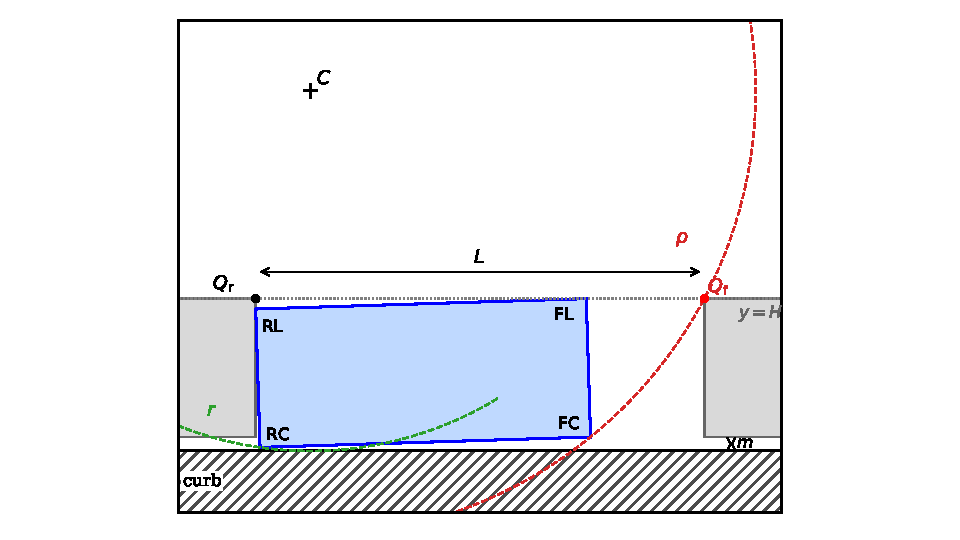
\includegraphics[width=0.85\textwidth]{figures/fig_geometry.pdf}
\caption{The slot (typical car, $L=\Lambda_1$).
The parked cars (grey) occupy $m\le y\le H$; the curb is hatched.
Our car is shown in the optimal one-manoeuvre position $q_d$ of \cref{thm:one}.
Under full left lock it rotates about $C$: the front curb-side corner $\cFC$ moves on the circle of radius $\rho$ through $\Qf$ (red), and the rear curb-side corner $\cRC$ on the circle of radius $r$ tangent to the curb (green).}
\label{fig:geometry}
\end{figure}

\subsection{Elementary properties}

\begin{lemma}[time reversal]\label{lem:reversal}
If $q$ is a manoeuvre of direction $d$ and length $S$, then $\tilde q(s)=q(S-s)$ is a manoeuvre of direction $-d$.
Consequently, a parking motion with $n$ manoeuvres exists if and only if an \emph{exit motion} with $n$ manoeuvres exists, i.e.\ a free motion from a parked configuration to a lane configuration.
\end{lemma}
\begin{proof}
$\tilde\psi(s)=\psi(S-s)$ is $1/R$-Lipschitz, and
\[
  \tilde P(s)=P(S)-d\int_{S-s}^{S}\e(\psi)=\tilde P(0)+(-d)\int_0^s\e(\tilde\psi(\sigma))\dd\sigma.
\]
Reversing the order of the manoeuvres of a parking motion gives an exit motion and conversely.
\end{proof}

From now on we mostly work with exits, which are easier to visualise: the car drives \emph{out} of the slot.

\begin{lemma}[monotonicity]\label{lem:monoL}
If $L\le L'$ then $\Free\subset\mathcal F_{L'}$; hence free, parked and lane configurations for $L$ are also free, parked and lane configurations for $L'$.
The set of slot lengths admitting a parking motion with at most $n$ manoeuvres is therefore an up-set.
Moreover $\Lmin(n+1)\le\Lmin(n)$.
\end{lemma}
\begin{proof}
Only $\Of$ depends on $L$, and it shrinks as $L$ grows.
A motion with at most $n$ manoeuvres also has at most $n+1$.
\end{proof}

\begin{lemma}[mirror symmetry]\label{lem:mirror}
The map $\mu_L(x,y,\psi)=(L-x,\,y,\,\pi-\psi)$ satisfies $\fp(\mu_L q)=\sigma(\fp(q))$ for the reflection $\sigma(x,y)=(L-x,y)$.
It maps manoeuvres to manoeuvres of the same direction and preserves the classes of free, parked and lane configurations.
\end{lemma}
\begin{proof}
The linear part of $\sigma$ sends $\e(\psi)$ to $\e(\pi-\psi)$ and $\n(\psi)$ to $-\n(\pi-\psi)$.
Since $\fp_0$ is symmetric under $v\mapsto -v$, $\sigma(\fp(P,\psi))=\fp(\sigma P,\pi-\psi)$.
Also $(\sigma P)'=d\,\e(\pi-\psi)$, so $\mu_L$ maps manoeuvres to manoeuvres of the same direction.
Finally $\sigma$ preserves $\mathcal C$ and the lane, and swaps $\Or$ and $\Of$.
\end{proof}

\begin{lemma}[parked cars are nearly level]\label{lem:fit}
Assume $H<\ell$ and let $\psi_{\rm fit}\in(0,\arctan(\ell/w))$ be the root of $\ell\sin\psi+w\cos\psi=H$.
If $q$ is parked, then $\psi$ lies within $\psi_{\rm fit}$ of a multiple of $\pi$.
\end{lemma}
\begin{proof}
The vertical extent of the footprint is $\ell|\sin\psi|+w|\cos\psi|$, and it must be at most $H$.
On $[0,\pi/2]$ the function $f(\psi)=\ell\sin\psi+w\cos\psi$ increases from $w<H$ to $\sqrt{\ell^2+w^2}$ and then decreases to $\ell>H$.
Hence $\{f\le H\}\cap[0,\pi/2]=[0,\psi_{\rm fit}]$, and the other quadrants follow by symmetry.
\end{proof}

Shifting the heading by a multiple of $2\pi$ changes nothing, and \cref{lem:mirror} maps headings near odd multiples of $\pi$ to headings near even ones.
We may and do therefore assume that the parked configuration at which an exit starts has $|\psi|\le\psi_{\rm fit}$.

\subsection{A soft curb}\label{sec:model-soft}
Ordinary curbs are lower than the bumpers and sills of a car.
The bodywork may then overhang the curb, and only the tyres have to stay on the road.
We call this the \emph{soft-curb model}, and the model above the \emph{rigid-curb model}.
In plan view each tyre is a rectangle aligned with the car, and in body coordinates the four tyres occupy
\[
  \W_0=\big([-\lambda,\lambda]\cup[d_w-\lambda,d_w+\lambda]\big)\times\big([-T_o,-T_o+t_w]\cup[T_o-t_w,T_o]\big).
\]
Here $\lambda$ is half the length of a tyre, $t_w$ its width and $T_o$ the distance of the outer sidewalls from the axis of the car.
We assume $\W_0\subset\fp_0$, i.e.\ $\lambda\le\min(d_b,d_f)$ and $T_o\le w/2$, and write $\delta_s=w/2-T_o\ge0$ for the inset of the outer sidewalls.

In the soft-curb model a configuration $q$ is \emph{free} if $\fp(q)\cap(\Or\cup\Of)=\emptyset$ and $\W(q)\cap\mathcal C=\emptyset$, where $\W(q)$ is the image of $\W_0$ under the rigid motion that maps $\fp_0$ to $\fp(q)$.
Parked and lane configurations, parking motions and the minimal length $\Lmins(n)$ are defined as in \cref{def:fit}, with this notion of freeness.
A parked car may therefore overhang the curb, but it must still lie in $\{y\le H\}$.
Since $\W_0\subset\fp_0$, every configuration that is free in the rigid-curb model is free in the soft-curb model, and hence
\begin{equation}\label{eq:soft-le}
  \Lmins(n)\le\Lmin(n)\qquad\text{for every }n.
\end{equation}
\Cref{lem:reversal,lem:monoL} hold verbatim, and so does \cref{lem:mirror}, because $\W_0$ is symmetric under $v\mapsto-v$.

For numerical values we use the same tyres for every car: $\delta_s=0.0275$ m, $t_w=0.205$ m and $\lambda=0.25$ m.
This is a $205$ mm tyre whose outer sidewall is $2.75$ cm inside the body side, and $2\lambda$ is the chord of a tyre of diameter $0.63$ m at a curb height of $0.12$ m.
We do not turn the front tyres with the steering.
All motions behind our numerical values remain free when the front tyres are turned to the Ackermann angles of full lock (\cref{app:numerics}), so the upper bounds hold in that model too.
The soft-curb model is analysed in \cref{sec:soft}, and the two models are compared in \cref{sec:compare}.

\section{Geometric tools}\label{sec:toolkit}

\subsection{Turning centres}
The \emph{left} and \emph{right turning centres} of a configuration $q=(P,\psi)$ are
\[
  C=P+R\,\n(\psi),\qquad C'=P-R\,\n(\psi).
\]
Under full left (right) lock the car rotates rigidly about $C$ ($C'$).

\begin{lemma}[drift of the centres]\label{lem:drift}
Along a manoeuvre of direction $d$, $C$ and $C'$ are Lipschitz, and for almost every $s$
\[
  \frac{\dd C}{\dd s}=(d-R\psi')\,\e(\psi),\qquad \frac{\dd C'}{\dd s}=(d+R\psi')\,\e(\psi).
\]
Since $|R\psi'|\le1$, the left centre moves along $d\,\e(\psi)$ with speed $|d-R\psi'|\in[0,2]$.
It stands still exactly when the car turns with full left lock ($\psi'=d/R$) and moves at speed $2$ under full right lock.
The analogous statements hold for $C'$.
\end{lemma}
\begin{proof}
$\frac{\dd}{\dd s}\n(\psi)=-\psi'\e(\psi)$ and $P'=d\,\e(\psi)$.
\end{proof}

\begin{lemma}[corners in polar form]\label{lem:polar}
Let $\gamma\in(0,\pi/2)$ and $\beta\in(0,\pi/2)$ be given by $(\cos\gamma,\sin\gamma)=(b,\Rp)/\rho$ and $(\cos\beta,\sin\beta)=(\Rp,d_b)/r$.
Then
\[
  \cFC=C+\rho\,\e(\psi-\gamma),\quad \cRC=C+r\,\e\big(\psi-\tfrac\pi2-\beta\big),\quad
  \cFL=C'+\rho\,\e(\psi+\gamma),\quad \cRL=C'+r\,\e\big(\psi+\tfrac\pi2+\beta\big).
\]
Moreover $|\cFL-C|=\sqrt{b^2+\Rm^2}<\rho$ and $|\cRL-C|=\sqrt{d_b^2+\Rm^2}<r$.
In particular
\begin{equation}\label{eq:RCy}
  \cRC_y=C_y-r\cos(\psi-\beta),\qquad \cFC_y=C_y+\rho\sin(\psi-\gamma).
\end{equation}
\end{lemma}
\begin{proof}
$\cFC-C=b\,\e-\Rp\,\n$, and $\e(\psi-\gamma)=\cos\gamma\,\e(\psi)-\sin\gamma\,\n(\psi)$.
The other identities are checked in the same way.
\end{proof}

\begin{lemma}[disk containment]\label{lem:disk}
If $d_b\le b$, the footprint $\fp(q)$ is contained in the closed disk of radius $\rho$ about $C$.
If $d_b<b$, the corner $\cFC$ is its only point on the boundary circle.
\end{lemma}
\begin{proof}
The footprint is the convex hull of its corners, the disk is convex, and by \cref{lem:polar} the corners have distances $\rho,r,\sqrt{b^2+\Rm^2},\sqrt{d_b^2+\Rm^2}$ from $C$.
These are at most $\rho$, with equality only for $\cFC$ when $d_b<b$; the farthest points of a convex polygon from a point are vertices.
\end{proof}

\subsection{The distance identity}
The next identity is our main tool.
It says that the left centre does not move away from any point lying ahead of the rear axle when the car moves forward, nor from any point behind the rear axle when it reverses.

\begin{lemma}[distance identity]\label{lem:distance}
Let $Q\in\R^2$ be fixed.
Along a manoeuvre of direction $d$, for almost every $s$,
\[
  \frac{\dd}{\dd s}|C-Q|^2=-2\,(d-R\psi')\,(Q-P)\cdot\e(\psi).
\]
In particular, for a forward manoeuvre $|C-Q|$ is non-increasing on every interval on which $(Q-P)\cdot\e(\psi)\ge0$, and for a reverse manoeuvre on every interval on which $(Q-P)\cdot\e(\psi)\le0$.
\end{lemma}
\begin{proof}
By \cref{lem:drift}, $\frac{\dd}{\dd s}|C-Q|^2=2(d-R\psi')(C-Q)\cdot\e$.
Moreover $(C-Q)\cdot\e=(P-Q)\cdot\e$ because $\n\cdot\e=0$.
Finally $d-R\psi'$ has the sign of $d$ or vanishes.
\end{proof}

\subsection{Full-lock arcs}
Under forward full left lock ($\psi'=1/R$) the centre $C$ is fixed and $\psi(s)=\psi(0)+s/R$.
Every body point therefore rotates counter-clockwise about $C$ on a circle, through the angle $\psi(s)-\psi(0)$.
Under reverse full right lock the car rotates counter-clockwise about the fixed $C'$.
Reverse full left lock and forward full right lock are clockwise rotations about $C$ and $C'$ respectively.

\subsection{Bounds for parked configurations}
Put
\[
  X(\psi)=d_b\cos\psi-\Rm\sin\psi,\qquad Y(\psi)=\Rm\cos\psi-b\sin\psi .
\]

\begin{lemma}\label{lem:parked}
Assume $H<\ell$ and $\cos\psi_{\rm fit}>m/w$, and let $q$ be parked with $|\psi|\le\psi_{\rm fit}$.
\begin{enumerate}[label=(\alph*)]
\item If $\psi\ge0$, then $P_x\ge d_b\cos\psi+\tfrac w2\sin\psi$ and $d_b\sin\psi+\tfrac w2\cos\psi\le P_y\le H-b\sin\psi-\tfrac w2\cos\psi$.
Hence
\[
  C_x\ge X(\psi),\qquad \Rp\cos\psi\le C_y\le H+Y(\psi).
\]
\item If $\psi<0$, then $P_x\ge d_b\cos\psi-\tfrac w2|\sin\psi|$; hence $C_x\ge d_b\cos\psi+\Rm|\sin\psi|$, $C'_x\ge d_b\cos\psi-\Rp|\sin\psi|$ and $\Rp\cos\psi\le C_y\le H+\Rm\cos\psi-d_b|\sin\psi|$.
\item The front of the car satisfies $\cFC_x\le L+m\tan|\psi|$ and $\cFL_x\le L$.
\end{enumerate}
\end{lemma}
\begin{proof}
(a) The lowest point is $\cRC$, so $\cRC_y\ge0$.
The highest point is $\cFL$, so $\cFL_y\le H$.
These two inequalities give the bounds on $P_y$.
Next, $\cRL_y=\cRC_y+w\cos\psi\ge w\cos\psi>m$ and $\cRL_y\le H$.
Points of the rear edge close to $\cRL$ therefore have heights in $(m,H)$ and lie outside $\Or$, so their $x$-coordinates are $\ge0$; by continuity $\cRL_x\ge0$.
Since $\cRL_x=P_x-d_b\cos\psi-\tfrac w2\sin\psi$, this is the bound on $P_x$.
The bounds on $C=P+R\n(\psi)$ follow.

(b) Now the highest point is $\cRL$, so $\cRL_y\le H$, which gives the upper bound on $C_y$.
The point $P-\tfrac w2\n$ of the footprint lies above the curb, so $P_y\ge\tfrac w2\cos\psi$ and $C_y=P_y+R\cos\psi\ge\Rp\cos\psi$.
As in (a), $\cRL_y\ge\cRC_y+w\cos\psi\ge w\cos\psi>m$ (here $\cRC_y\ge\cFC_y\ge0$), so $\cRL$ lies in the band or on its upper boundary and $\cRL_x\ge0$.
Since $\cRL=P-d_b\e+\tfrac w2\n$, this reads $P_x\ge d_b\cos\psi-\tfrac w2|\sin\psi|$, and the bounds on $C_x=P_x+R|\sin\psi|$ and $C'_x=P_x-R|\sin\psi|$ follow.

(c) The front edge runs from $\cFC$ to $\cFL=\cFC+w\,\n(\psi)$.
We have $\cFL_y\le H$, because the footprint lies below $H$.
Also $\cFL_y=\cFC_y+w\cos\psi\ge w\cos\psi>m$, using $\cFC_y\ge0$ and $\cos\psi\ge\cos\psi_{\rm fit}>m/w$.
Hence $\cFL$ lies in the band (or on its upper boundary), and by continuity $\cFL_x\le L$.
If $\psi\le0$, then $\cFC_x=\cFL_x-w|\sin\psi|\le L$.
If $\psi>0$ and $\cFC_y>m$, then $\cFC$ lies in the band and $\cFC_x\le L$.
If $\psi>0$ and $\cFC_y\le m$, the front edge meets the height $m$ at the point $\cFC+t\,\n(\psi)$ with $t=(m-\cFC_y)/\cos\psi$.
Points of the edge just above it lie in the band, so this point has $x\le L$, i.e.\ $\cFC_x-t\sin\psi\le L$.
Since $t\le m/\cos\psi$, this gives $\cFC_x\le L+m\tan\psi$.
\end{proof}

\section{One manoeuvre}\label{sec:one}

\subsection{Statement}
Recall $X(\psi)=d_b\cos\psi-\Rm\sin\psi$ and $Y(\psi)=\Rm\cos\psi-b\sin\psi$.
Let
\[
  \varepsilon_b=r-\Rp=\sqrt{d_b^2+\Rp^2}-\Rp
\]
be the \emph{rear swing}: the amount by which the rear curb-side corner dips below its starting height when a car parked level drives forward with full left lock.
When $H<\ell$ (which follows from \ref{A:fit} below), let $\psi_b\in(0,\pi/2)$ be defined by $\sin\psi_b=H/\ell$, and put $c_2=2b/\sin\psi_b$.
Since $Y$ is strictly decreasing on $[0,\pi/2]$, the equation
\begin{equation}\label{eq:psid}
  Y(\psi_d)=r-H
\end{equation}
has a unique solution $\psi_d\in[0,\pi/2)$ as soon as $Y(0)=\Rm\ge r-H$, i.e.\ as soon as $m\ge\varepsilon_b$.

\begin{assumption}\label{ass:one}
\leavevmode
\begin{enumerate}[label=(A\arabic*),nosep]
\item\label{A:db} $d_b<b$, $\Rp^2>bd_b$, and $m\ge\varepsilon_b$;
\item\label{A:fit} $H<b$, $H<\Rm+d_b$, $\cos\psi_b>m/w$, $\psi_{\rm fit}<\beta$, $\Rp\cos\psi_{\rm fit}>\max(H,\Rm)$ and $\Rm\ge d_b\tan(\psi_{\rm fit}/2)$;
\item\label{A:nose} $2Rb>w\rho$, $wb>m\rho$ and $b\rho>H\Rp$;
\item\label{A:curbcase} $(\Rp^2-bd_b)/r\ge r-H$;
\item\label{A:min} $\cos\psi_d\sqrt{b^2+2Rw}>\Rm\sin\psi_d+b$ and
 \[
   b\cos\psi_{\rm fit}\,\big(2Y(\psi_{\rm fit})+c_2\big)>2(\Rm+d_b\sin\psi_{\rm fit})\sqrt{\rho^2+c_2\,\big(r-H-Y(\psi_{\rm fit})\big)};
 \]
\item\label{A:end} $r-d_b\ge H$ and $X(\psi_d)\ge0$;
\item\label{A:far} $d_b\cos\psi_{\rm fit}-\Rp\sin\psi_{\rm fit}+\rho\ge\Lambda_1$ and $B_{\rm back}\ge\Lambda_1$, where $\Lambda_1$ is defined in \eqref{eq:Lambda1def} below and $B_{\rm back}$ in \eqref{eq:Bback}.
\end{enumerate}
\end{assumption}

These are mild ``realistic car'' inequalities.
\Cref{app:assumptions} checks them for the typical car of \cref{tab:values} and on a grid of 1280 parameter sets covering passenger cars, with $m=w/10$.
They fail mainly when $m<\varepsilon_b$ (an unusually long rear overhang combined with a very tight turning circle), and otherwise only for very short and wide cars.
Only \ref{A:db} and \ref{A:end} enter the upper bound; the other conditions serve the lower bound.

\begin{theorem}\label{thm:one}
Under \cref{ass:one},
\begin{equation}\label{eq:Lambda1def}
  \Lmin(1)=\Lambda_1:=X(\psi_d)+\sqrt{\rho^2-(r-H)^2}.
\end{equation}
Equivalently, with $\varsigma=r-H$ and $s_0^2=b^2+\Rm^2$,
\[
  \Lambda_1=\frac{\ell\,\Rm\,\varsigma+(bd_b-\Rm^2)\sqrt{s_0^2-\varsigma^2}}{s_0^2}+\sqrt{\rho^2-\varsigma^2}.
\]
The infimum is attained.
An optimal exit starts from the parked configuration $q_d$ with heading $\psi_d$ whose lane-side corners touch the line $y=H$ and the car behind ($\cFL_y=H$, $\cRL_x=0$).
It drives forward with full left lock, during which the front curb-side corner grazes $\Qf$ and the rear curb-side corner grazes the curb, and then straightens with full right lock.
\end{theorem}

The closed form follows from \eqref{eq:psid}: writing $(\Rm,b)=s_0(\cos\chi,\sin\chi)$ we get $\psi_d+\chi=\arccos(\varsigma/s_0)$, hence
$\cos\psi_d=(\varsigma\Rm+b\sqrt{s_0^2-\varsigma^2})/s_0^2$ and $\sin\psi_d=(\Rm\sqrt{s_0^2-\varsigma^2}-\varsigma b)/s_0^2$.

\begin{corollary}[classical formula]\label{cor:classical}
Under \cref{ass:one}, if $m=\varepsilon_b$, then $\psi_d=0$ and $\Lmin(1)=d_b+\sqrt{b^2+2Rw}=d_b+\sqrt{(d_w+d_f)^2+(R+\tfrac w2)^2-(R-\tfrac w2)^2}$.
For $m>\varepsilon_b$ the value $\Lambda_1$ is strictly smaller.
\end{corollary}
\begin{proof}
For $m=\varepsilon_b$ we have $r-H=\Rm$, so $\psi_d=0$, $X(0)=d_b$ and $\rho^2-\Rm^2=b^2+2Rw$.
If $m>\varepsilon_b$, then $\psi_d>0$, and the first inequality of \ref{A:min} shows that $\psi\mapsto X(\psi)+\sqrt{\rho^2-Y(\psi)^2}$ is strictly decreasing on $[0,\psi_d]$; hence $\Lambda_1$ is smaller than its value at $\psi=0$, which is the classical length.
\end{proof}

For the typical car of \cref{tab:values}: $\varepsilon_b=0.069<m=0.18$, $\psi_d=0.0314$ rad $=1.80^\circ$, $\Lambda_1=5.833$~m, while the classical value is $5.861$~m.
In driving terms, the optimal \emph{parking} manoeuvre (time-reversed) reverses with full right lock, then reverses with full left lock, and stops while the car is still turned $1.8^\circ$ nose-up (see \cref{fig:one}).

\begin{figure}[ht]
\centering
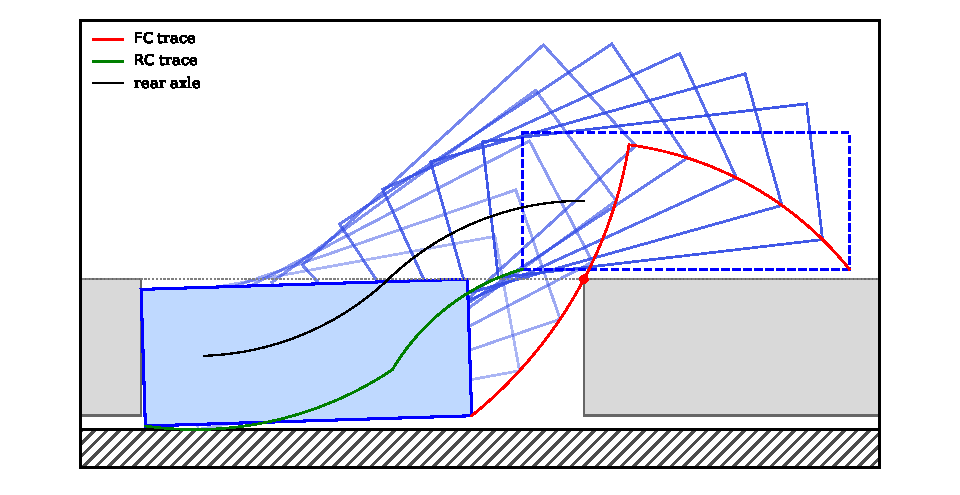
\includegraphics[width=0.85\textwidth]{figures/fig_one.pdf}
\caption{The optimal single manoeuvre for the typical car, drawn as an exit: full left lock from $q_d$ (filled) up to the heading $0.76$ rad, then full right lock to the level lane position (dashed).
Read backwards, it is the parking manoeuvre: reverse with right lock, then with left lock.
The front curb-side corner (red trace) grazes $\Qf$; the rear curb-side corner (green trace) grazes the curb.}
\label{fig:one}
\end{figure}

\subsection{The upper bound}

\begin{proposition}\label{prop:one-upper}
Assume \ref{A:db} and \ref{A:end}, and let $L=\Lambda_1$.
Let $q_d=(P,\psi_d)$ with $P=\big(d_b\cos\psi_d+\tfrac w2\sin\psi_d,\ H-b\sin\psi_d-\tfrac w2\cos\psi_d\big)$.
Then $q_d$ is parked.
The exit consisting of forward full left lock from heading $\psi_d$ to $\pi/2$, followed by forward full right lock from $\pi/2$ to $0$, is free and ends in a lane configuration.
Hence $\Lmin(1)\le\Lambda_1$.
\end{proposition}

\begin{proof}
For $q_d$ the left centre is
\[
  C=P+R\n(\psi_d)=\big(X(\psi_d),\,H+Y(\psi_d)\big)=\big(X(\psi_d),\,r\big)
\]
by \eqref{eq:psid}.
By construction $\cFL_y=H$ and $\cRL_x=0$.

\emph{$q_d$ is parked.}
The highest point is $\cFL$ and the leftmost is $\cRL$, so the footprint lies in $\{y\le H\}\cap\{x\ge0\}$.
By \eqref{eq:RCy} the lowest point satisfies $\cRC_y=r-r\cos(\psi_d-\beta)\ge0$.
For the front, $\cFC=C+\rho\,\e(\psi_d-\gamma)$ lies on the circle of radius $\rho$ about $C$, below the height $H$.
The point of that circle at height $H$ on its right half is $(\Lambda_1,H)=\Qf$, because $C_y-H=r-H$ and $\Lambda_1-C_x=\sqrt{\rho^2-(r-H)^2}$.
Moving along the lower right quarter of the circle towards $\Qf$ increases $x$, so $\cFC_x<L$.
Since $\cFC$ is the rightmost point, the footprint lies in $\{x\le L\}$, hence in $\Free$.

\emph{First arc.}
During forward full left lock the footprint rotates counter-clockwise about the fixed point $C$ through the angle $\pi/2-\psi_d$ (\cref{sec:toolkit}).
\begin{itemize}[nosep]
\item \emph{Front.} By \cref{lem:disk} the footprint stays in the closed disk $D$ of radius $\rho$ about $C$.
If $p=(p_x,p_y)\in\Of$, then $p_x-C_x>L-C_x\ge0$ and $C_y-p_y>C_y-H\ge0$, so $|p-C|^2>|\Qf-C|^2=\rho^2$.
Thus $\Of\cap D=\emptyset$.
\item \emph{Rear and curb.} At the start every point of the footprint lies strictly below $C$, since $y\le H<r=C_y$ by \ref{A:end}.
Consider a point at polar angle $\vartheta_0\in(\pi,2\pi)$ about $C$; during the arc its angle is $\vartheta_0+t$ with $t\in[0,\pi/2-\psi_d]$.
\begin{itemize}[nosep]
\item If $\vartheta_0\in(\pi,3\pi/2]$, the angle stays in $(\pi,2\pi)$, where $\cos$ is increasing, so the point moves right and keeps $x\ge0$.
\item If $\vartheta_0\in(3\pi/2,2\pi)$, the angle stays in $(3\pi/2,5\pi/2)$, where $\cos\ge0$, so $x\ge C_x=X(\psi_d)\ge0$.
\end{itemize}
Hence no point enters $\Or$.
For the curb, points with $\vartheta_0\in(3\pi/2,2\pi)$ only rise.
A point with $\vartheta_0\in(\pi,3\pi/2]$ has body coordinates $(u,v)$ with $u\cos\psi_d-(v-R)\sin\psi_d\le0$, hence $u\le0$.
Its distance from $C$ is therefore at most $\sqrt{d_b^2+\Rp^2}=r$, so its height never drops below $C_y-r=0$.
\end{itemize}

\emph{End of the first arc.}
At heading $\pi/2$ we have $P=C+(R,0)$, and a body point $(u,v)$ sits at $C+(R-v,u)$.
Its height is $C_y+u\ge r-d_b\ge H$ by \ref{A:end}, so the car is in the lane.

\emph{Second arc.}
Forward full right lock rotates the car clockwise about $C'=C+(2R,0)$.
All points have $x\le C_x+R+w/2<C'_x$ when the arc starts.
Along a clockwise rotation, the height of each point is a unimodal function of time (it rises until the point passes the top of its circle).
It therefore stays above the minimum of its initial and final heights.
The final configuration is level with rear axle at height $C_y+R$, so all its points have $y\ge r+\Rm>H$.
Hence the car remains in the lane and ends parallel to the curb.
\end{proof}

\begin{remark}
The quarter turn is chosen for ease of proof.
Any switching heading $\alpha\ge\alpha_{\min}$ between left and right lock gives a valid exit.
For the typical car the binding constraint is that the final level position lies in the lane, $r+\Rm-2R\cos\alpha\ge H$, so $\alpha_{\min}=\arccos\big((r+\Rm-H)/(2R)\big)=0.734$ rad ($42.0^\circ$); a numerical collision check finds no other active constraint.
These are the familiar S-shaped parking paths: in forward time one reverses with right lock and then with left lock.
\end{remark}

\subsection{Lower bound for forward exits}

\begin{proposition}\label{prop:one-forward}
Suppose that \cref{ass:one} holds.
If a forward manoeuvre leads from a parked configuration $q_0$ with $|\psi(0)|\le\psi_{\rm fit}$ to a lane configuration through free configurations, then $L\ge\Lambda_1$.
\end{proposition}

\begin{proof}
Suppose $L<\Lambda_1$.
Write $q(s)=(P(s),\psi(s))$, $s\in[0,S]$, and let $C(s)$, $C'(s)$ be the turning centres.

\emph{Step 1: the crossing time.}
At the end the whole car lies in $\{y\ge H\}$, so $\cFC_y(S)\ge H$.
At the start $\cFC_y(0)=\cFL_y(0)-w\cos\psi(0)<H$.
Let $\tau=\min\{s:\cFC_y(s)=H\}$.

\emph{Step 2: heading bounds on $[0,\tau]$.}
Let $s_*\le\tau$ be the supremum of the times $t\le\tau$ such that $-\gamma<\psi<\psi_b$ on $[0,t)$; it is positive because $|\psi(0)|\le\psi_{\rm fit}<\min(\gamma,\psi_b)$.
Indeed $\psi_{\rm fit}<\beta<\gamma$ by \ref{A:fit} and \ref{A:db} (the second inequality is equivalent to $\Rp^2>bd_b$), and $\ell\sin\psi_{\rm fit}=H-w\cos\psi_{\rm fit}<H$ gives $\psi_{\rm fit}<\psi_b$.
In particular $\cos\psi_{\rm fit}>\cos\psi_b>m/w$ by \ref{A:fit}, so \cref{lem:parked} applies.
We first collect consequences valid on $[0,s_*)$.
\begin{itemize}
\item[(i)] Whenever $\psi\in[0,\pi/2]$ the lowest point is $\cRC$, so $P_y\ge d_b\sin\psi+\tfrac w2\cos\psi$ and hence $\cFC_y\ge\ell\sin\psi$.
For $s<\tau$ this gives $\ell\sin\psi<H$, i.e.\ $\psi<\psi_b$ whenever $\psi\in[0,\pi/2]$.
\item[(ii)] If $\psi(s)\in[0,\psi_b)$ then $P_y=\cFC_y-b\sin\psi+\tfrac w2\cos\psi<H+\tfrac w2$.
Since $P_y'=\sin\psi$ and $\psi>-\gamma>-\pi$, $P_y$ decreases on intervals where $\psi<0$; also $P_y(0)<H+w/2$.
Hence $P_y<H+w/2$ on $[0,s_*)$, and by continuity $P_y(s_*)\le H+w/2$.
\item[(iii)] On $[0,s_*)$ we have $\cos\psi>0$, so by \cref{lem:drift} $C'_x$ is non-decreasing on $[0,s_*]$.
Moreover $C'_x(0)=P_x(0)+R\sin\psi(0)\ge d_b\cos\psi_{\rm fit}-\Rp\sin\psi_{\rm fit}$.
For $\psi(0)\ge0$ this follows from \cref{lem:parked}(a), and for $\psi(0)<0$ from \cref{lem:parked}(b).
\end{itemize}
Now suppose $\psi(t)=-\gamma$ for some $t\le s_*$ (by continuity this is the only way $-\gamma<\psi$ can fail at $s_*$).
By \cref{lem:polar}, $\cFL(t)=C'(t)+(\rho,0)$, so by (iii) and \ref{A:far},
\[
  \cFL_x(t)\ge d_b\cos\psi_{\rm fit}-\Rp\sin\psi_{\rm fit}+\rho\ge\Lambda_1>L .
\]
Its height is $\cFL_y=P_y-R\cos\gamma\le H+\tfrac w2-\tfrac{Rb}\rho<H$ by (ii) and \ref{A:nose}.
If $\cFL_y>m$, then $\cFL\in\Of$.
Otherwise $\cFC_y=\cFL_y-w\cos\gamma\le m-wb/\rho<0$ by \ref{A:nose}, and the car meets the curb.
Both are impossible.
Likewise $\psi(s_*)=\psi_b$ with $s_*<\tau$ is excluded by (i).
Hence $s_*=\tau$, and $-\gamma<\psi(\tau)\le\psi_b$.

\emph{Step 3: $\psi(\tau)\in[0,\psi_b]$.}
If $\psi(\tau)\in(-\gamma,0)$, the lowest point is $\cFC$, at height $H$.
Then $P_y(\tau)=H+b|\sin\psi|+\tfrac w2\cos\psi$, while $P_y(\tau)\le H+w/2$ by (ii).
This gives $\tan(|\psi|/2)\ge 2b/w>1$ (note $2b>w$ by \ref{A:nose}), contradicting $|\psi|<\pi/2$.

\emph{Step 4: $\cFC_x(\tau)\le L$.}
For $s<\tau$ close to $\tau$ the height of $\cFC(s)$ lies in $(m,H)$.
Since $\cFC(s)\notin\Of$, $\cFC_x(s)\le L$, and we let $s\uparrow\tau$.

\emph{Step 5: $\Qf$ stays ahead of the rear axle.}
We claim that for $s\in[0,\tau]$
\begin{equation}\label{eq:ahead}
  (\Qf-P)\cdot\e(\psi)\ \ge\ b-H\sin\gamma>0,\qquad\text{and}\qquad (\Qf-P)\cdot\e(\psi)\ge b\ \text{ if }\psi\ge0 .
\end{equation}
Write $(\Qf-P)\cdot\e=(L-\cFC_x)\cos\psi+(H-\cFC_y)\sin\psi+b$, and note $H-\cFC_y\ge0$.

If $\psi\ge0$ and $\cFC_y>m$, then $\cFC_x\le L$, and both terms are $\ge0$.
If $\psi\ge0$ and $\cFC_y\le m$, the front edge rises from $\cFC$ in direction $\n(\psi)$ to $\cFL$, with $\cFL_y=\cFC_y+w\cos\psi\in(m,H]$ by \ref{A:fit}.
Its point at height $m$ has $x\le L$, so $L-\cFC_x\ge-(m-\cFC_y)\tan\psi$.
Then $(L-\cFC_x)\cos\psi+(H-\cFC_y)\sin\psi\ge(H-m)\sin\psi=w\sin\psi\ge0$.

If $\psi<0$, the front edge rises from $\cFC$ in direction $\n(\psi)=(|\sin\psi|,\cos\psi)$ to $\cFL$, so $\cFC_x\le\cFL_x$.
If $\cFL_y\le m$ then $\cFC_y=\cFL_y-w\cos\psi<0$, which is impossible; here $w\cos\psi>w\cos\gamma=wb/\rho>m$ by \ref{A:nose}.
If $\cFL_y\in(m,H)$ then $\cFC_x\le\cFL_x\le L$.
If $\cFL_y\ge H$, the point of the front edge at height $H$ has $x\le L$, and it lies to the right of $\cFC$.
In all cases $\cFC_x\le L$, and $(H-\cFC_y)|\sin\psi|\le H\sin\gamma$ because $\cFC_y\ge0$ and $|\psi|<\gamma$.
The positivity of $b-H\sin\gamma=b-H\Rp/\rho$ is \ref{A:nose}.

\emph{Step 6: the corner is far from the centre at time $\tau$.}
At $\tau$, $\Qf=\cFC(\tau)+(\delta,0)$ with $\delta=L-\cFC_x(\tau)\ge0$.
In body coordinates of $q(\tau)$ the point $\Qf$ is $(b+\delta\cos\psi,\,-\tfrac w2-\delta\sin\psi)$, and $C$ is $(0,R)$.
As $\psi(\tau)\in[0,\pi/2)$,
\[
  |C(\tau)-\Qf|^2=(b+\delta\cos\psi)^2+(\Rp+\delta\sin\psi)^2\ \ge\ \rho^2 .
\]

\emph{Step 7: curb cost.}
By \cref{lem:distance} and \eqref{eq:ahead}, on $[0,\tau]$
\[
  \frac{\dd}{\dd s}|C-\Qf|^2=-2(1-R\psi')(\Qf-P)\cdot\e\le0,\qquad \frac{\dd C_y}{\dd s}=(1-R\psi')\sin\psi .
\]
If $\psi\in(0,\psi_b)$, then $(\Qf-P)\cdot\e\ge b\ge(b/\sin\psi_b)\sin\psi$.
If $\psi\le0$, then $\frac{\dd C_y}{\dd s}\le0$.
In both cases $\frac{\dd}{\dd s}\big(|C-\Qf|^2+c_2C_y\big)\le0$ with $c_2=2b/\sin\psi_b$.
Consequently, for every $t\in[0,\tau]$,
\begin{equation}\label{eq:curbcost}
  |C(0)-\Qf|^2\ \ge\ |C(\tau)-\Qf|^2+c_2\big(C_y(t)-C_y(0)\big)\ \ge\ \rho^2+c_2\big(C_y(t)-C_y(0)\big).
\end{equation}
The first inequality holds because $|C-\Qf|^2$ is non-increasing on $[t,\tau]$ and $|C-\Qf|^2+c_2C_y$ is non-increasing on $[0,t]$.

\emph{Step 8: the curb forces $C_y\ge r$ at some time.}
By \eqref{eq:RCy} and the curb, $C_y(s)\ge r\cos(\psi(s)-\beta)$ for all $s$.
If $\psi$ takes the value $\beta$ on $[0,\tau]$, this gives $C_y\ge r$ there.
Otherwise $\psi<\beta$ on $[0,\tau]$, because $\psi(0)\le\psi_{\rm fit}<\beta$.
In that case \eqref{eq:RCy} at $\tau$ gives $C_y(\tau)=H+\rho\sin(\gamma-\psi(\tau))\ge H+\rho\sin(\gamma-\beta)$, using $0\le\psi(\tau)<\beta<\gamma$ ($\beta<\gamma$ is equivalent to $\Rp^2>bd_b$).
Now $\rho\sin(\gamma-\beta)=(\Rp^2-bd_b)/r\ge r-H$ by \ref{A:curbcase}.
Either way some $t\in[0,\tau]$ has $C_y(t)\ge r$, and \eqref{eq:curbcost} yields
\[
  (L-C_x(0))^2+(C_y(0)-H)^2=|C(0)-\Qf|^2\ \ge\ \rho^2+c_2\big(r-C_y(0)\big)^+ .
\]
Moreover $C_x(0)\le P_x(0)+R\sin\psi_{\rm fit}\le L-b\cos\psi_{\rm fit}+\Rp\sin\psi_{\rm fit}<L$.
Here we used \cref{lem:parked}(c), and $\tan\psi_{\rm fit}<\tan\beta=d_b/\Rp<b/\Rp$.
Taking square roots, we obtain
\begin{equation}\label{eq:Phi}
  L\ \ge\ \Phi(q_0):=C_x(0)+\sqrt{\rho^2-(C_y(0)-H)^2+c_2\big(r-C_y(0)\big)^+}.
\end{equation}

\emph{Step 9: minimisation over parked configurations.}
$\Phi$ is increasing in $C_x$ and, on $\{C_y\ge H\}$, decreasing in $C_y$.
If $\psi(0)\in[0,\psi_{\rm fit}]$, \cref{lem:parked}(a) gives $C_x\ge X(\psi)$ and $H<\Rp\cos\psi_{\rm fit}\le\Rp\cos\psi\le C_y\le H+Y(\psi)$, using \ref{A:fit}; so $\Phi(q_0)\ge\varphi_{\rm c}(\psi(0))$ with
\[
  \varphi_{\rm c}(\psi):=X(\psi)+\sqrt{\rho^2-Y(\psi)^2+c_2\big(r-H-Y(\psi)\big)^+}.
\]
If $\psi(0)<0$, \cref{lem:parked}(b) gives $H<\Rp\cos\psi_{\rm fit}\le C_y\le H+\Rm$ and $C_x\ge d_b\cos\psi+\Rm|\sin\psi|\ge d_b$.
The last inequality is equivalent to $\Rm\ge d_b\tan(|\psi|/2)$, which holds by \ref{A:fit}.
Hence $\Phi(q_0)\ge\varphi_{\rm c}(0)$.
Finally $\psi_d\le\psi_{\rm fit}$, because $q_d$ is parked (\cref{prop:one-upper,lem:fit}), and $\varphi_{\rm c}$ is decreasing on $[0,\psi_d]$ and increasing on $[\psi_d,\psi_{\rm fit}]$.
On $[0,\psi_d]$ the penalty vanishes and the derivative of $X+\sqrt{\rho^2-Y^2}$ is at most
\[
  -\Rm\cos\psi_d+\Rm(\Rm\sin\psi_d+b)/\sqrt{b^2+2Rw}<0
\]
by \ref{A:min}.
On $[\psi_d,\psi_{\rm fit}]$ the derivative is positive by the second inequality of \ref{A:min}.
Hence $L\ge\varphi_{\rm c}(\psi_d)=X(\psi_d)+\sqrt{\rho^2-(r-H)^2}=\Lambda_1$, a contradiction.
\end{proof}

\subsection{Lower bound for reverse exits}

For a reverse exit we follow the height of the curb-side end of the rear axle, i.e.\ of the point $P-\tfrac w2\n$,
\[
  h=P_y-\tfrac w2\cos\psi\qquad(|\psi|<\pi/2).
\]
For a reverse manoeuvre, $h'=-\sin\psi\,(1-\tfrac w2\psi')$ with $1-\tfrac w2\psi'\in[\Rm/R,\Rp/R]$.
So $h$ increases only while the car points nose-down, and then the curb limits the rate of increase.
Let $\psi_n=\arcsin(H/b)$ and $c_\psi=\cos\psi_n$, and let $\psi_u\in(0,\pi/2)$ solve $\Rm(1-\cos\psi_u)+d_b\sin\psi_u=H$; it exists since $\Rm+d_b>H$.
Put $h_0=H-w\cos\psi_{\rm fit}$ and
\begin{equation}\label{eq:Bback}
  B_{\rm back}=b\cos\psi_{\rm fit}-\tfrac w2\sin\psi_{\rm fit}+\min\big(f_b(-\psi_n),f_b(\psi_u)\big)+c_\psi\frac{Rb}{\Rp}\log^+\frac{Hb}{\ell h_0},
\end{equation}
where $f_b(\psi)=d_b\cos\psi-\tfrac w2\sin\psi$.

\begin{proposition}\label{prop:one-reverse}
Assume \ref{A:fit}.
If a reverse manoeuvre leads from a parked configuration with $|\psi(0)|\le\psi_{\rm fit}$ to a lane configuration through free configurations, then $L\ge B_{\rm back}$.
\end{proposition}

\begin{proof}
Let $\tau_r$ be the first time at which $\cRC_y=H$.
It exists because $\cRC_y(0)<H$ and the car ends in the lane.
At the start, $h(0)\le H-w\cos\psi(0)\le h_0<H$, because the highest point of the parked car is at most $H$.

\emph{Heading bounds.}
Let $s_1$ be the first time with $|\psi|=\pi/2$, and work on $[0,\min(s_1,\tau_r))$.
\begin{itemize}[nosep]
\item On intervals with $\psi<0$ we have $\cRC_y=h+d_b|\sin\psi|<H$, so $h<H$.
On intervals with $\psi\ge0$, $h$ does not increase.
Hence $h<H$ throughout.
\item If $\psi\le0$, the lowest point is $\cFC$, with $\cFC_y=h-b|\sin\psi|\ge0$.
Hence $|\sin\psi|\le h/b<H/b$ and $\psi>-\psi_n$.
\item Let $I=(s_a,s_b)$ be a maximal interval on which $\psi>0$, and suppose $\psi$ first reaches $\psi_u$ at $t\in I$.
Since $|\psi'|\le1/R$,
\[
  \int_{s_a}^t\sin\psi\dd s\ \ge\ R\int_{s_a}^t\sin\psi\,|\psi'|\dd s\ \ge\ R\big(\cos\psi(s_a)-\cos\psi_u\big).
\]
Therefore $h(t)\le h(s_a)-\Rm(\cos\psi(s_a)-\cos\psi_u)$.
If $s_a>0$ then $\psi(s_a)=0$ and $h(s_a)<H$.
If $s_a=0$, then $h(0)\le H-w\cos\psi_{\rm fit}$ and $\cos\psi(0)\ge\cos\psi_{\rm fit}$, so $h(t)\le H-\Rp\cos\psi_{\rm fit}+\Rm\cos\psi_u<H-\Rm(1-\cos\psi_u)$ because $\Rp\cos\psi_{\rm fit}>\Rm$.
In both cases $h(t)<H-\Rm(1-\cos\psi_u)=d_b\sin\psi_u$.
This contradicts $\cRC_y(t)=h(t)-d_b\sin\psi_u\ge0$.
\end{itemize}
Thus $\psi\in(-\psi_n,\psi_u)\subset(-\pi/2,\pi/2)$ before $\min(s_1,\tau_r)$; hence $s_1>\tau_r$, and the bounds hold on $[0,\tau_r]$.

\emph{Gronwall.}
On intervals where $\psi<0$, we get $h'\le(\Rp/R)|\sin\psi|\le(\Rp/(Rb))\,h$.
Elsewhere $h$ does not increase.
Hence $h(\tau_r)\le h_0\exp\big(\tfrac{\Rp}{Rb}S_-\big)$, where $S_-$ is the total length of the intervals where $\psi<0$.
At $\tau_r$: if $\psi\le0$ then $H=\cRC_y=h+d_b|\sin\psi|\le h\,\ell/b$; if $\psi>0$ then $H=h-d_b\sin\psi<h$.
So $h(\tau_r)\ge Hb/\ell$, and $S_-\ge\frac{Rb}{\Rp}\log^+\frac{Hb}{\ell h_0}$ (trivially if $Hb\le\ell h_0$).

\emph{Room.}
$P_x'=-\cos\psi\le0$, and $P_x'\le-c_\psi$ while $\psi<0$.
So $P_x(0)-P_x(\tau_r)\ge c_\psi S_-$.
By \cref{lem:parked}(c), $P_x(0)\le L-b\cos\psi_{\rm fit}+\tfrac w2\sin\psi_{\rm fit}$.
Just before $\tau_r$ the corner $\cRC$ is in the band and outside $\Or$, so $\cRC_x(\tau_r)\ge0$.
Hence $P_x(\tau_r)\ge f_b(\psi(\tau_r))\ge\min\big(f_b(-\psi_n),f_b(\psi_u)\big)$.
The last step holds because $f_b(\psi)=\sqrt{d_b^2+w^2/4}\,\cos(\psi+\chi_b)$ with $\chi_b=\arctan(w/(2d_b))\in(0,\pi/2)$, and for $\psi\in(-\pi/2,\pi/2)$ the argument $\psi+\chi_b$ lies in $(-\pi/2,\pi)$, where $\cos$ increases and then decreases; so on any interval the minimum is attained at an end point.
Combining these inequalities gives $L\ge B_{\rm back}$.
\end{proof}

For the typical car $B_{\rm back}\approx8.2$ m, far above $\Lambda_1$: driving out forwards (i.e.\ parking in reverse) is much better, as every driver knows.

\begin{proof}[Proof of \cref{thm:one}]
By \cref{lem:mirror} every one-manoeuvre exit can be transformed into one starting with $|\psi(0)|\le\psi_{\rm fit}$ and with the same direction.
\Cref{prop:one-forward,prop:one-reverse} and \ref{A:far} show $L\ge\Lambda_1$ for every one-manoeuvre exit, and \cref{prop:one-upper} provides an exit for $L=\Lambda_1$.
By \cref{lem:reversal} the same holds for parking.
\end{proof}

\subsection{Why the margin is needed}\label{sec:flush}

The problem is often posed with a slot exactly as deep as the car is wide, the car finishing flush against the curb.
In our notation this is $m=0$; we extend the definitions of \cref{sec:model} to this case.
Then $H=w$, and since $\ell>w$ the vertical extent $\ell|\sin\psi|+w|\cos\psi|$ of the footprint is at most $w$ only if $\psi\in\pi\mathbb Z$; so a parked configuration has $\psi\in\pi\mathbb Z$ and $P_y=w/2$.

\begin{proposition}[flush parking is impossible]\label{prop:flush}
Let $m=0$, $\ell>w$ and $d_b>0$.
Consider a motion through configurations whose footprints lie in $\{y\ge0\}$, with any number of manoeuvres, that ends at a flush configuration (heading $0$, $P_y=w/2$).
Then the car was flush and moving along the curb throughout: $\psi\equiv0$ and $P_y\equiv w/2$.
In particular no parking motion exists, and $\Lmin(n)=+\infty$ for every $n$ (a parking motion ending with heading $\pi$ is reduced to this case by \cref{lem:mirror}).
\end{proposition}

\begin{proof}
Parametrise the concatenated motion by total arc length $s\in[0,T]$, so that $P_y$ is Lipschitz with $|P_y'|=|\sin\psi|$ almost everywhere.
Let $y=P_y-w/2$ and $c=\min(d_b,b,w/2)>0$.
For $|\psi|\le\pi/2$ the lowest point of the footprint is $\cRC$ or $\cFC$, so the curb constraint reads
\[
  y\ \ge\ \max(d_b\sin\psi,\,-b\sin\psi)-\tfrac w2(1-\cos\psi)\ \ge\ c|\sin\psi|-\tfrac w2\sin^2\psi ,
\]
using $1-\cos\psi\le\sin^2\psi$ there.
Hence $y\ge\frac c2|\sin\psi|$ whenever $|\sin\psi|\le c/w$.
In that regime $|y'|=|\sin\psi|\le\frac2c\,y$.

Let $t_*=\inf\{t\le T:\ |\sin\psi|\le c/w\text{ on }[t,T]\}$.
Since $c/w\le1/2$, the set $\{|\sin\psi|\le c/w\}$ consists of intervals of half-width at most $\pi/6$ around the multiples of $\pi$; as $\psi(T)=0$ and $\psi$ is continuous, $|\psi|\le\pi/6$ on $[t_*,T]$, so the bound above applies there.
On $[t_*,T]$ we have $y\ge0$, $y(T)=0$ and $y(s)\le\frac2c\int_s^Ty$.
Gronwall's inequality gives $y\equiv0$ there, hence $\sin\psi\equiv0$ and, by continuity, $\psi\equiv0$.
If $t_*>0$, continuity of $\psi$ at $t_*$ contradicts the definition of $t_*$.
So $t_*=0$.
\end{proof}

Physically, the rear overhang swings towards the curb whenever the car turns.
Approaching a wall tangentially with the whole side therefore takes infinitely long: the distance to the wall can shrink at most exponentially in the distance driven.
With a margin $m>0$ the car need not touch the curb, and the problem becomes well posed.
Margins of the order of the rear swing $\varepsilon_b$ (a few centimetres) suffice for the one-manoeuvre analysis; $m=w/10$ is comfortably larger for ordinary cars.

\section{Several manoeuvres}\label{sec:several}

\subsection{The escape length}
For a configuration $q$ with left centre $C$ satisfying $|C_y-H|\le\rho$, define the \emph{escape length}
\[
  V(q)=C_x+\sqrt{\rho^2-(C_y-H)^2}.
\]
It is the abscissa at which the front curb-side corner would cross the height $H$ if the car drove forward with full left lock from $q$.
The proof of \cref{prop:one-forward} shows that (under \cref{ass:one}) a forward exit from a parked configuration $q$ requires $L\ge V(q)$; heuristically the same holds for low, nearly level configurations.
Conversely, $V(q)\le L$ suffices when the curb and the rear are not in the way.
By \cref{lem:drift}, $C$ moves only along $\pm\e(\psi)$, which yields the following bookkeeping:
\begin{itemize}[nosep]
\item forward or reverse \emph{full left lock} leaves $C$, and hence $V$, unchanged;
\item reverse motion moves $C$ backwards, so $V$ decreases (as long as $\psi$ is moderate), fastest under full right lock, where $C$ moves at speed $2$;
\item forward motion without full left lock moves $C$ forwards and increases $V$.
\end{itemize}
A good multi-manoeuvre exit therefore alternates two kinds of manoeuvre.
Reverse arcs with full right lock lower $V$ and turn the car nose-up.
Forward arcs with full left lock keep $V$ fixed, create room behind the car and also turn it nose-up.
The reverse arcs are limited by the curb and by the car behind, the forward arcs by the car in front.
The final manoeuvre is a forward full-left-lock exit, possible once $V\le L$.

\subsection{Two manoeuvres}

\begin{proposition}\label{prop:two}
Let $\alpha\in(0,\pi/2)$ be the solution of
\begin{equation}\label{eq:alpha2}
  \Rm(1-\cos\alpha)+d_b\sin\alpha=m ,
\end{equation}
and put
\[
  \Lambda_2=d_b\cos\alpha-\Rm\sin\alpha+\sqrt{\rho^2-(2R\cos\alpha-\Rp)^2}.
\]
Assume $\Rm+d_b>m$, $d_b<b$, $\alpha\ge\beta$, $d_b\cos\alpha\ge\Rm\sin\alpha$, $r\cos(\alpha-\beta)-d_b\ge H$, $d_b\cos\alpha+\Rp\sin\alpha+b\le\Lambda_2$, $\max(b,d_b)\tan\alpha<\Rm$ and $\Rp\ge d_b\tan(\alpha/2)$.
Then $\Lmin(2)\le\Lambda_2$.
\end{proposition}

The left-hand side of \eqref{eq:alpha2} increases from $0$ to $\Rm+d_b>m$ on $[0,\pi/2]$, so $\alpha$ is well defined.
(The inequality $2R\cos\alpha\ge\Rp$ used below follows from $C_{1,y}=r\cos(\alpha-\beta)\ge H+d_b$.)
For the typical car, $\alpha=0.1732$ rad $=9.93^\circ$, $\beta=0.1717$ rad and $\Lambda_2=5.4247$~m, and all hypotheses hold; the thinnest margin is $\alpha-\beta=0.0015$ rad.
The two-manoeuvre gap is thus $0.41$ m shorter than the one-manoeuvre gap.

\begin{proof}
We describe an exit with $L=\Lambda_2$; see \cref{fig:two}.
Let $x_0=d_b\cos\alpha+\Rp\sin\alpha$ and start from the level configuration $q_0=((x_0,m+\tfrac w2),0)$.
It is parked: its footprint is $[x_0-d_b,x_0+b]\times[m,H]$, with $x_0-d_b=\sin\alpha\,(\Rp-d_b\tan\frac\alpha2)\ge0$ and $x_0+b\le L$ by assumption.

\emph{Manoeuvre 1: reverse with full right lock through the angle $\alpha$.}
The car rotates counter-clockwise about the fixed right centre $C'=(x_0,m+\tfrac w2-R)$.
After rotating by $t\in[0,\alpha]$, a body point $(u,v)$ sits at $C'$ plus the vector $(u,v+R)$ rotated by $t$.
That vector has vertical component $u\sin t+(v+R)\cos t\ge\Rm\cos t-d_b\sin t>0$, because $d_b\tan\alpha<\Rm$.
So every point stays above $C'$ and moves to the left. Moreover:
\begin{itemize}[nosep]
\item the leftmost point $\cRL$ has $x=x_0-d_b\cos t-\Rp\sin t\ge0$, with equality at $t=\alpha$, so the car never enters $\Or$;
\item the lowest point $\cRC$ has height $m-\Rm(1-\cos t)-d_b\sin t\ge0$, with equality at $t=\alpha$; its abscissa $x_0-d_b\cos t-\Rm\sin t$ decreases in $t$ and ends at $w\sin\alpha\ge0$;
\item the front moves away from $\Of$.
\end{itemize}
At the end, $q_1=(P_1,\alpha)$ with $P_1=C'+R(-\sin\alpha,\cos\alpha)$.
Both rear corners are in contact: $\cRC$ with the curb and $\cRL$ with the car behind.
The left centre of $q_1$ is
\[
  C_1=\big(x_0-2R\sin\alpha,\ m+\tfrac w2-R+2R\cos\alpha\big)=\big(d_b\cos\alpha-\Rm\sin\alpha,\ H+2R\cos\alpha-\Rp\big).
\]

\emph{Manoeuvre 2: forward with full left lock to heading $\pi/2$, then full right lock to heading $0$.}
We follow the proof of \cref{prop:one-upper} with $C_1$ in place of $C$.
\begin{itemize}[nosep]
\item By the choice of $L$, $|C_1-\Qf|=\rho$; also $C_{1,x}\le L$ and $C_{1,y}\ge H$, so $\Of$ misses the disk of radius $\rho$ about $C_1$.
\item Every point of the car is below $C_1$: the highest point $\cFL$ lies below $C_1$ by $\Rm\cos\alpha-b\sin\alpha>0$. Since also $C_{1,x}\ge0$, no point enters $\Or$ (polar-angle argument).
\item For the curb: by \eqref{eq:RCy}, $0=\cRC_y(q_1)=C_{1,y}-r\cos(\alpha-\beta)$.
Since $\alpha\ge\beta$, $\cRC$ has already passed the bottom of its circle and now rises.
The points that still pass through the bottom of their circles have body coordinates with $u<-(R-v)\tan\alpha$.
Their distance from $C_1$ is less than $|u|/\sin\alpha\le d_b/\sin\alpha$.
Since $\sin\alpha\cos(\alpha-\beta)-\sin\beta=\tfrac12\big(\sin(2\alpha-\beta)-\sin\beta\big)\ge0$ for $\beta\le\alpha\le\pi/2$, we get $d_b/\sin\alpha\le r\cos(\alpha-\beta)=C_{1,y}$.
Hence these points stay above the curb.
\item At heading $\pi/2$ the lowest point has height $C_{1,y}-d_b=r\cos(\alpha-\beta)-d_b\ge H$, and the final right-lock arc keeps the car in the lane as in \cref{prop:one-upper}.
\end{itemize}
This is a free exit with two manoeuvres; \cref{lem:reversal} turns it into a parking motion.
\end{proof}

In driving terms (forward time) the strategy is the familiar one.
Reverse in along an S-curve (right lock, then left lock) and stop when the car, turned $\alpha\approx10^\circ$ nose-up, touches the curb with its rear corner and the car behind with its rear bumper.
Then pull forward with full right lock until the car is level.

\begin{figure}[ht]
\centering
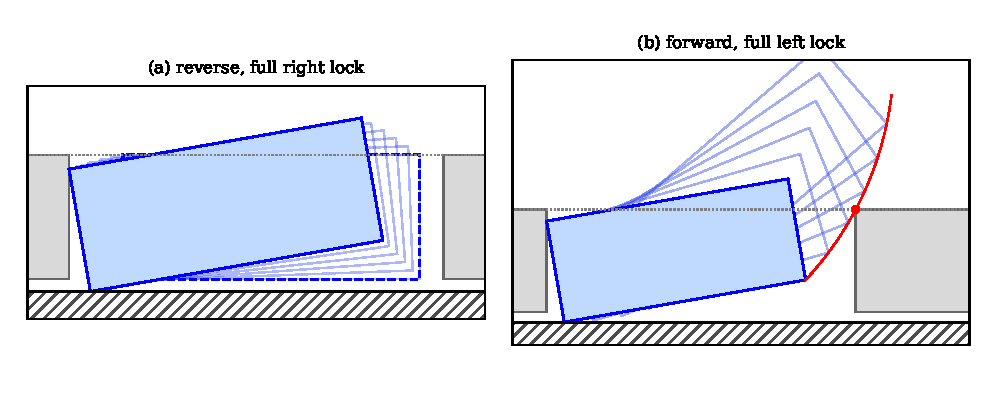
\includegraphics[width=\textwidth]{figures/fig_two.pdf}
\caption{The two-manoeuvre exit of \cref{prop:two} for the typical car ($L=\Lambda_2$).
(a) Reverse with full right lock from the level position (dashed) until both rear corners touch.
(b) Forward exit with full left lock; the front curb-side corner (red) grazes $\Qf$.}
\label{fig:two}
\end{figure}

\begin{remark}\label{rem:two-other}
If $\alpha<\beta$, stopping the reversal at the double contact would make the rear corner dip into the curb during the exit.
One then stops the reversal at the angle $\alpha_d\le\alpha$ given by $2R\cos\alpha_d=r+\Rp-H$, so that $C_{1,y}=r$, and chooses $x_0=d_b\cos\alpha_d+\Rp\sin\alpha_d$; the angle exists when $r+\Rp-H\le2R$, i.e.\ when $m\ge\varepsilon_b$.
This gives $\Lmin(2)\le d_b\cos\alpha_d-\Rm\sin\alpha_d+\sqrt{\rho^2-(r-H)^2}$, provided the analogues of the hypotheses of \cref{prop:two} hold at $\alpha_d$: $X(\alpha_d)\ge0$, $r-d_b\ge H$, $x_0+b\le L$, $\max(b,d_b)\tan\alpha_d<\Rm$ and $\Rp\ge d_b\tan(\alpha_d/2)$.
The proof is that of \cref{prop:two}, except that the curb step of the exit is now the argument of \cref{prop:one-upper}: $C_{1,y}=r$, and the points that pass the bottom of their circles are at distance at most $r$ from $C_1$.
\end{remark}

\subsection{A better two-manoeuvre exit}\label{sec:two-better}

\Cref{prop:two} does not use the room in front of the car.
Starting further forward and first reversing briefly with \emph{left} lock tilts the car nose-down by a small angle $a_0$.
The subsequent right-lock arc then runs from $-a_0$ to a slightly larger final tilt $\alpha_1>\alpha$.
The left centre drops by about the same amount as in \cref{prop:two}, because in both cases the curb contact pins $C_{1,y}$ near $r$, but it moves back further: $2R(\sin a_0+\sin\alpha_1)$ instead of $2R\sin\alpha$.
With the larger final tilt this gives a smaller $C_{1,x}=X(\alpha_1)$, and hence a shorter slot.
The optimal choice makes three contacts: the front bumper with the car in front at the start, and, at the end of the reverse manoeuvre, the two rear corners with the curb and with the car behind.

\begin{proposition}\label{prop:two-better}
Suppose that $\alpha_1\in[\beta,\pi/2)$ and $a_0\in(0,\pi/2)$ solve
\begin{align}
  2R\cos a_0&=H+\Rm(1+\cos\alpha_1)-d_b\sin\alpha_1, \label{eq:tc1}\\
  b+2R(\sin a_0+\sin\alpha_1)&=\sqrt{\rho^2-\big(r\cos(\alpha_1-\beta)-H\big)^2}, \label{eq:tc2}
\end{align}
and put $\Lambda_2^*=b+2R\sin a_0+d_b\cos\alpha_1+\Rp\sin\alpha_1$.
Assume in addition $d_b<b$, $\gamma+a_0\le\pi/2$, $H+\Rm\ge\rho\sin(\gamma+a_0)$, $d_b\cos\alpha_1\ge\Rm\sin\alpha_1$, $r\cos(\alpha_1-\beta)-d_b\ge H$, $\Rp\ge d_b\tan(\alpha_1/2)$, and
\[
  \max(b,d_b)\tan a_0<\Rm,\qquad \Rm\tan a_0<d_b,\qquad \max(b,d_b)\tan\alpha_1<\Rm .
\]
Then $\Lmin(2)\le\Lambda_2^*$.
\end{proposition}

For the typical car, $a_0=0.04116$ rad, $\alpha_1=0.17815$ rad and $\Lambda_2^*=5.4104$ m.
This improves on $\Lambda_2=5.4247$.

\begin{proof}
Let $L=\Lambda_2^*$ and start from the level configuration with $P_0=(L-b,\,m+\tfrac w2)$.
It is parked, and its front bumper touches the car in front.

\emph{Reverse with full left lock by $a_0$.}
This is a clockwise rotation about the left centre $C_0=(L-b,\,H+\Rm)$.
The car stays below $C_0$ throughout, since its highest corner $\cRL$ lies below $C_0$ by $\Rm\cos\psi-d_b|\sin\psi|>0$ (because $d_b\tan a_0<\Rm$).
Hence all points have negative $x$-velocity, and the car moves away from the car in front.
The lowest point is $\cFC$, at height $C_{0,y}+\rho\sin(\psi-\gamma)$, which decreases to $C_{0,y}-\rho\sin(\gamma+a_0)\ge0$ by assumption.
The rear rises.
For heading $\psi\in[-a_0,0]$ the leftmost corner is $\cRC=C_0+r\,\e(\psi-\frac\pi2-\beta)$, with abscissa $C_{0,x}-d_b\cos\psi-\Rp|\sin\psi|\ge L-\ell-\Rp\sin a_0$.
By the definition of $\Lambda_2^*$,
\[
  L-\ell=2R\sin a_0+\sin\alpha_1\big(\Rp-d_b\tan\tfrac{\alpha_1}2\big)\ \ge\ 2R\sin a_0\ \ge\ \Rp\sin a_0 .
\]
Hence the car stays clear of $\Or$.

\emph{Reverse with full right lock from heading $-a_0$ to $\alpha_1$.}
This is a counter-clockwise rotation about the right centre
\[
  C'_a=C_0-2R\big(\sin a_0,\cos a_0\big)=\big(L-b-2R\sin a_0,\ H+\Rm-2R\cos a_0\big).
\]
A body point has position $C'_a$ plus the vector $(u,v+R)$ rotated by $\psi$; its vertical component relative to $C'_a$ is $u\sin\psi+(v+R)\cos\psi\ge\Rm\cos\psi-\max(b,d_b)|\sin\psi|>0$ for $\psi\in[-a_0,\alpha_1]$.
So every point stays above $C'_a$ and moves left.
Relative to $C'_a$ the corners $\cRC$ and $\cRL$ have body coordinates $(-d_b,\Rm)$ and $(-d_b,\Rp)$.
Hence
\[
  \cRC_y=C'_{a,y}-d_b\sin\psi+\Rm\cos\psi,\qquad \cRL_x=C'_{a,x}-d_b\cos\psi-\Rp\sin\psi .
\]
Both are strictly decreasing for $\psi\in[-a_0,\alpha_1]$.
For $\cRC_y$ the derivative $-d_b\cos\psi-\Rm\sin\psi$ is negative because $\tan a_0<d_b/\Rm$.
For $\cRL_x$ the derivative $d_b\sin\psi-\Rp\cos\psi$ is negative because $\tan\alpha_1<\Rm/d_b<\Rp/d_b$.
By \eqref{eq:tc1}, $\cRC_y=0$ exactly at $\psi=\alpha_1$; by the definition of $\Lambda_2^*$, $\cRL_x=0$ exactly at $\psi=\alpha_1$.
So both contacts occur only at the end.
While $\psi<0$ the lowest point is $\cFC$; it lies to the right of $C'_a$ and therefore rises.
The leftmost corner is then $\cRC$, with abscissa $C'_{a,x}-d_b\cos\psi+\Rm|\sin\psi|\ge C'_{a,x}-d_b=L-\ell-2R\sin a_0\ge0$.
The front moves away from $\Of$.

\emph{Forward exit.}
Composing the two rotations, the left centre at heading $\alpha_1$ is $C_1=C'_a+2R\,\n(\alpha_1)$.
By the definition of $\Lambda_2^*$ and by \eqref{eq:tc1}, this gives
\[
  C_1=\big(d_b\cos\alpha_1-\Rm\sin\alpha_1,\ \Rp\cos\alpha_1+d_b\sin\alpha_1\big)=\big(d_b\cos\alpha_1-\Rm\sin\alpha_1,\ r\cos(\alpha_1-\beta)\big).
\]
Equation \eqref{eq:tc2} is equivalent to $|C_1-\Qf|=\rho$.
The rest of the argument is the proof of \cref{prop:two} verbatim, with $\alpha_1$ in place of $\alpha$.
\end{proof}

In forward time the second manoeuvre pulls forward with full right lock until the car points slightly nose-down, then with full left lock until it is level and touches the car in front.

\subsection{Three or more manoeuvres}\label{sec:zigzag}

For $n\ge3$ we use \emph{rotation zigzags}.
The exit alternates forward full-left-lock arcs and reverse manoeuvres, ending with the forward escape.
A reverse manoeuvre is a full-right-lock arc, possibly preceded by a short full-left-lock arc (of at most $0.1$ rad), as in \cref{prop:two-better}.
For odd $n$ it starts with a forward arc, for even $n$ with a reverse arc.
The free parameters are the starting position and the length of each arc as a fraction of the maximal collision-free length.
We optimised them numerically for the typical car (\cref{app:numerics}); \cref{tab:zigzag} lists the results.
The car turns further nose-up at every manoeuvre and gains clearance from the curb, which in turn permits a longer next reverse arc.

\begin{table}[ht]
\centering
\begin{tabular}{lcccccc}
\toprule
$n$ & 1 & 2 & 3 & 4 & 5 & 6\\
\midrule
upper bound for $\Lmin(n)$ [m] & 5.833 & 5.411 & 5.280 & 5.180 & 5.050 & 4.978\\
\bottomrule
\end{tabular}
\caption{Best rotation-zigzag strategies found for the typical car ($n=1$ exact, $n=2$ from \cref{prop:two-better}; the search for $n=6$ was stopped early). Upper bounds are rounded up.}
\label{tab:zigzag}
\end{table}

\Cref{fig:values} compares these values with the crawl of \cref{sec:asym}.
\Cref{app:five,app:twenty} show a five- and a twenty-manoeuvre parking motion in detail, and \cref{app:cars} gives values for other cars.

How far can rotation alone go?
In the \emph{greedy} zigzag every arc is driven until contact, and the car escapes as soon as $V\le L$.
For the typical car it needs $2,3,4,8,14$ manoeuvres for slack $g=1.3,1.1,0.9,0.7,0.6$ m respectively.
For $g\le0.5$ m it stalls: the car stops turning before it can escape.

\begin{figure}[ht]
\centering
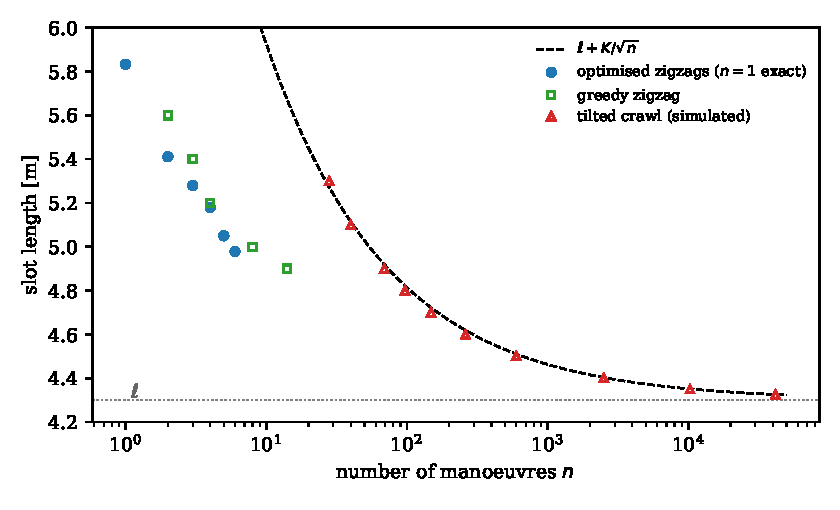
\includegraphics[width=0.8\textwidth]{figures/fig_values.pdf}
\caption{Slot lengths achieved with $n$ manoeuvres for the typical car.
All points are upper bounds for $\Lmin(n)$, except $n=1$, which is exact.
Filled circles: optimised rotation zigzags; squares: greedy zigzags; triangles: simulated tilted crawls.
The dashed curve is the sharp asymptotics $\ell+K/\sqrt n$ of \cref{thm:asym}.
Rotation is far more efficient for few manoeuvres; the crawl is asymptotically optimal.}
\label{fig:values}
\end{figure}

For large $n$ the rotation mechanism is exhausted.
Once the gap is only slightly longer than the car, every exit stays nearly level until the car has almost left the slot (\cref{lem:confine}).
Progress then comes from lateral \emph{crawling}, analysed in \cref{sec:asym}.

\begin{conjecture}\label{conj:two}
For the typical car, $\Lmin(2)=\Lambda_2^*$.
\end{conjecture}

The evidence is numerical.
We ran differential-evolution searches over exits consisting of a reverse manoeuvre followed by a forward full-left-lock escape.
The reverse manoeuvre was made of up to three arcs of arbitrary curvature and length, with arbitrary starting position, height and tilt.
Exits that begin with a forward manoeuvre end in reverse and were not searched.
At $L=5.40$ m they found no feasible two-manoeuvre exit.
The searches over left-then-right full-lock reverse arcs converge to the triple contact of \cref{prop:two-better}.
A proof would need a calibration adapted to the three contact constraints, in the spirit of \cref{sec:asym}.

\section{Many manoeuvres: sharp asymptotics}\label{sec:asym}

\subsection{Statements}
For $g>0$ let $N(g)$ be the least number of manoeuvres of a parking motion for the slot length $L=\ell+g$, with $N(g)=\infty$ if there is none.
By \cref{lem:monoL}, $N$ is non-increasing.
Under the hypotheses of \cref{thm:asym} no parked configuration exists when $L<\ell$: the argument of \cref{lem:confine}(ii) below gives $f(|\psi|)\le L-\ell$ for a function $f\ge0$.
Hence $\Lmin(n)\ge\ell$, and $\Lmin(n)=\ell+\inf\{g>0:\ N(g)\le n\}$.

\begin{theorem}\label{thm:mono}
$\Lmin(n)$ is non-increasing in $n$.
Under the hypotheses of \cref{thm:asym}, moreover $\ell<\Lmin(n)\le\Lmin(1)$ for every $n$, and $\Lmin(n)\to\ell$ as $n\to\infty$.
\end{theorem}

Some hypothesis such as $H<\ell$ is needed for $\Lmin(n)>\ell$.
If $\ell\le H$, a car can turn in the lane and drive nose-first straight down into the slot; it is then parked with heading $-\pi/2$ in a slot of length about $w<\ell$.

\begin{theorem}\label{thm:asym}
Assume the standing assumption $R>w/2$, $0<m<w$, $H<\ell$, $d_b\le b$, and
\begin{equation}\label{eq:mcond}
  m<\frac{2w\cos^2\psi_{\rm fit}}{1+2\cos\psi_{\rm fit}}
\end{equation}
(which holds, for instance, whenever $m\le w/2$ and $\ell\ge2w$). Put
\[
  r_*(u)=\begin{cases}\dfrac1{4R}, & 0\le u\le \tfrac w2,\\[8pt] \dfrac{R}{4\big(R^2-(u-\frac w2)^2\big)}, & \tfrac w2\le u\le w,\end{cases}
  \qquad K^2=\int_0^w\frac{\dd u}{r_*(u)}=4Rw-\frac{w^3}{6R}.
\]
Then $\lim_{g\downarrow0}g^2N(g)=K^2$; consequently $\sqrt n\,(\Lmin(n)-\ell)\to K$ as $n\to\infty$.
\end{theorem}

Here $u$ measures how far the car has been lifted out of the slot, and $g^2r_*(u)$ is the largest lift per manoeuvre achievable at height $u$, to leading order.
The two theorems are proved in \cref{sec:asym-proofs}.
The main steps:
\begin{enumerate}[nosep]
\item a \emph{confinement lemma}: until the car is almost out, the heading stays $O(g)$ along every exit;
\item an exact description of the free configurations in rescaled variables: a parallelogram (\emph{window});
\item a \emph{calibration}: a function $G$ on the window such that the lift in one manoeuvre is at most $g^2(r_*+\Delta G)$ up to $O(g^3)$;
\item a matching construction by tilted S-curves.
\end{enumerate}

\subsection{Rescaled variables}
Fix the slack $g\in(0,1]$ and write $L=\ell+g$.
For a configuration $q=(P,\psi)$ set
\[
  u=P_y-\tfrac w2-m,\qquad \xi=\frac{P_x-d_b}{g},\qquad \phi=\frac{\psi}{g}.
\]
For a level car, $u$ is the height of its curb-side edge above the curb-side edges of the parked cars.
A parked level car has $u\le0$, and a level car in the lane has $u\ge w$.
Along a manoeuvre of direction $d$,
\begin{equation}\label{eq:lift}
  \frac{\dd u}{\dd s}=d\sin\psi,\qquad \frac{\dd P_x}{\dd s}=d\cos\psi,\qquad\text{hence}\qquad \dd u=\tan\psi\,\dd P_x=g^2\,\frac{\tan\psi}{\psi}\,\phi\,\dd\xi .
\end{equation}
Moreover $\dd\phi/\dd\xi=\psi'/(d\cos\psi)\in[-1/(R\cos\psi),\,1/(R\cos\psi)]$.
So, to leading order, the rescaled state $(\xi,\phi)$ moves along curves of slope at most $1/(R\cos\psi)$ in absolute value; $\xi$ increases in forward manoeuvres and decreases in reverse ones.
The lift is the area-like integral $g^2\int\phi\,\dd\xi$.

\subsection{Confinement}

\begin{lemma}[confinement]\label{lem:confine}
Let $0<\delta\le w/4$.
Put $c=\max(4/\delta,\,4/(w-m))$, and choose $\psi_1\in(0,\delta/(2b)]$ so small that
\[
  (w-m\sec\psi_1)\Big(1-\frac{\psi_1^2}6\Big)-\frac{\ell\psi_1}2\ \ge\ \frac{w-m}2,\qquad \cos\psi_1>\frac mw,\qquad \frac{w\psi_1^2}{4}<\frac\delta4 .
\]
There is $g_0>0$ (depending on $\delta$ and the parameters) such that for $0<g\le g_0$:
\begin{enumerate}[label=(\roman*)]
\item no free configuration has $u\le w-\delta$ and $cg\le|\psi|\le\psi_1$;
\item every parked configuration has $|\psi|<cg$ (heading taken modulo $\pi$ as in \cref{lem:fit});
\item along every exit motion, $|\psi|<cg$ holds up to the first time $T_\delta$ at which $u\ge w-\delta$, and $T_\delta$ exists.
\end{enumerate}
\end{lemma}

\begin{proof}
(i) Let $q$ be free with $u\le w-\delta$ and $\psi\in[cg,\psi_1]$ (nose-up); the nose-down case is symmetric and treated at the end.
The corner heights are
\[
\begin{aligned}
  \cRC_y&=m+u+\tfrac w2(1-\cos\psi)-d_b\sin\psi, & \cFC_y&=m+u+\tfrac w2(1-\cos\psi)+b\sin\psi,\\
  \cRL_y&=m+u+w-\tfrac w2(1-\cos\psi)-d_b\sin\psi, & \cFL_y&=\cRL_y+\ell\sin\psi .
\end{aligned}
\]
The leftmost point is $\cRL$ and the rightmost is $\cFC$.
Since $\cRC_y\ge0$, we have $\cRL_y\ge w\cos\psi>m$, so $\cRL$ is never in the gap.

\emph{Case a: $\cFC_y\ge H$.}
Then $u\ge w-b\sin\psi-\tfrac w2(1-\cos\psi)>w-b\psi_1-\tfrac w4\psi_1^2>w-\delta$, which is excluded.

\emph{Case b: $\cFC_y\in(m,H)$ and $\cRL_y<H$.}
Both extreme corners lie in the band, so $\cFC_x\le L$ and $\cRL_x\ge0$.
This gives $\ell\cos\psi+w\sin\psi\le\ell+g$.
Using $\sin\psi\ge\psi(1-\psi^2/6)$ and $1-\cos\psi\le\psi^2/2$, we get $\psi\,\big(w(1-\psi_1^2/6)-\ell\psi_1/2\big)\le g$.
The bracket is at least $(w-m)/2$, so $\psi\le 2g/(w-m)<cg$, a contradiction.

\emph{Case c: $\cFC_y\in(m,H)$ and $\cRL_y\ge H$.}
The band part of the rear edge ends at height $H$, at the point with abscissa $P_x-d_b\sec\psi-(H-P_y)\tan\psi$, which must be $\ge0$.
Together with $\cFC_x\le L$ and $H-P_y=\tfrac w2-u$, this yields after multiplication by $\cos\psi$
\[
  \sin\psi\Big[\tfrac w2(1+\cos\psi)-u\Big]\ \le\ g\cos\psi+(1-\cos\psi)(b\cos\psi-d_b).
\]
Divide by $\sin\psi$ and use $u\le w-\delta$, $g\cot\psi\le g/\psi\le1/c\le\delta/4$ and $\tan(\psi/2)\le\psi\le\psi_1$.
This gives $\delta-\tfrac w4\psi_1^2\le\delta/4+b\psi_1\le\delta/4+\delta/2$, contradicting $w\psi_1^2/4<\delta/4$.

\emph{Case d: $\cFC_y\le m$.}
Then $u<0$, so $\cRL_y<H$ and $\cRL_x\ge0$.
The front edge rises from $\cFC$ to $\cFL$ with $\cFL_y=\cFC_y+w\cos\psi\in(m,H]$, so its point at height $m$ has abscissa $\cFC_x-(m-\cFC_y)\tan\psi\le L$.
Hence $\ell\cos\psi+w\sin\psi-m\tan\psi\le\ell+g$, and therefore $\psi\big[(w-m\sec\psi_1)(1-\psi_1^2/6)-\ell\psi_1/2\big]\le g$.
This again gives $\psi\le2g/(w-m)<cg$.

\emph{Nose-down, $\psi\in[-\psi_1,-cg]$, $a=|\psi|$.}
Now the leftmost point is $\cRC$ (height $m+u+\tfrac w2(1-\cos a)+d_b\sin a$), the rightmost is $\cFL$ (height $m+u+w-\tfrac w2(1-\cos a)-b\sin a$), and $\cFL_y\ge w\cos a>m$.
\begin{itemize}[nosep]
\item If $\cRC_y\ge H$, then $u>w-\delta$.
\item If both $\cRC$ and $\cFL$ lie in the band, we argue as in case b.
\item If $\cRC$ lies in the band and $\cFL_y\ge H$, the band part of the front edge ends at height $H$, at abscissa $P_x+b\sec a+(H-P_y)\tan a\le L$.
With $P_x\ge d_b\cos a+\tfrac w2\sin a$ this gives $\sin a\big[\tfrac w2(1+\cos a)-u\big]\le g\cos a-(1-\cos a)(b-d_b\cos a)\le g\cos a$.
This is excluded as in case c, here without the $b\psi_1$ term.
\item If $\cRC_y\le m$, then $u<0$ and the rear edge's point at height $m$ has abscissa $\cRC_x+(m-\cRC_y)\tan a\ge0$.
With $\cFL_x\le L$ this is case d.
\end{itemize}

(ii) A parked configuration has $|\psi|\le\psi_{\rm fit}$ by \cref{lem:fit}, and since its highest point is at most $H$, it has $u\le\frac w2(1-\cos\psi_{\rm fit})<w-\delta$.
Cases b and d, applied to $\psi\in(0,\psi_{\rm fit}]$, and their nose-down analogues for $\psi\in[-\psi_{\rm fit},0)$ give $f(|\psi|)\le g$, where $f(\psi):=(w-m\sec\psi)\sin\psi-\ell(1-\cos\psi)$.
Now $f$ is positive on $(0,\psi_{\rm fit}]$.
Indeed, $f(\psi)>0$ is equivalent to $w-m\sec\psi>\ell\tan(\psi/2)$; the left side decreases and the right side increases in $\psi$.
At $\psi_{\rm fit}$, using $\ell\tan(\psi_{\rm fit}/2)=\ell\sin\psi_{\rm fit}/(1+\cos\psi_{\rm fit})=(m+w(1-\cos\psi_{\rm fit}))/(1+\cos\psi_{\rm fit})$, the inequality reduces to \eqref{eq:mcond}.
Moreover $f(\psi)\ge\frac{w-m}2\psi$ on $(0,\psi_1]$.
(Cases b and d use $\cos\psi>m/w$ for $\psi\le\psi_{\rm fit}$; this follows from \eqref{eq:mcond}, since $2c_f^2/(1+2c_f)<c_f$ for $c_f=\cos\psi_{\rm fit}\in(0,1]$.)
Hence for $g<\min_{[\psi_1,\psi_{\rm fit}]}f$ every parked configuration has $|\psi|\le 2g/(w-m)<cg$.

(iii) Choose $g_0$ such that (ii) holds and $cg_0<\psi_1$.
Along an exit motion $\psi$ is continuous and starts in $(-cg,cg)$.
If $|\psi|$ reached $cg$ at a first time $t_1<T_\delta$, then $q(t_1)$ would violate (i).
At the end the car is in the lane, so its lowest point is at height $\ge H$.
If $|\psi|<cg$ there, then $u\ge w-\max(b,d_b)\,cg-\tfrac w2c^2g^2>w-\delta$ (decreasing $g_0$ if necessary); otherwise $T_\delta$ has already occurred.
Hence $T_\delta$ exists.
\end{proof}

\subsection{Windows}
From now on $0<g\le g_0$ and $|\psi|<cg$, so $|\phi|<c$.
For $k\in[0,w/2]$ introduce the sheared coordinate
\[
  \zeta_k=\xi+k\phi .
\]
\begin{lemma}[windows]\label{lem:windows}
There is a constant $A$ (depending on $\delta$ and the parameters) with the following property, after decreasing $g_0$ if necessary.
Let $q$ be free with $|\psi|<cg$ and $0\le u\le w-\delta$, and let $k\in[0,w/2]$ satisfy $k\ge u-\tfrac w2$.
Then $-Ag\le\zeta_k\le1+Ag$.
\end{lemma}

\begin{proof}
Since $|\psi|<cg$ and $0\le u\le w-\delta$, for $g$ small:
\begin{itemize}[nosep]
\item nose-up, the leftmost corner $\cRL$ is in the band or above $H$, and the rightmost corner $\cFC$ is in the band;
\item nose-down, the leftmost corner $\cRC$ is in the band, and the rightmost corner $\cFL$ is in the band or above $H$.
\end{itemize}
(A corner in the gap is never extreme in these cases.)
The exact constraints are therefore, for $\psi\ge0$,
\[
  P_x\ \ge\ \min\big(d_b\cos\psi+\tfrac w2\sin\psi,\ d_b\sec\psi+(\tfrac w2-u)\tan\psi\big),\qquad P_x\le L-b\cos\psi-\tfrac w2\sin\psi,
\]
and for $\psi<0$, with $a=|\psi|$,
\[
  P_x\ \ge\ d_b\cos a+\tfrac w2\sin a,\qquad P_x\ \le\ L-\min\big(b\cos a+\tfrac w2\sin a,\ b\sec a+(\tfrac w2-u)\tan a\big).
\]
In each case the first expression applies when the lane-side corner is in the band, the second when it is above $H$; in both cases we use the weaker of the two bounds.
Expanding to first order in $\psi$, with $O(g^2)$ remainders uniform in the stated ranges, these give
\[
  \xi\ \ge\ \min\big(\tfrac w2,\tfrac w2-u\big)\phi-Ag,\quad \xi\le1-\tfrac w2\phi+Ag\qquad(\phi\ge0),
\]
\[
  \xi\ \ge\ \tfrac w2|\phi|-Ag,\quad \xi\le1-\min\big(\tfrac w2,\tfrac w2-u\big)|\phi|+Ag\qquad(\phi<0).
\]
Adding $k\phi$ and using $\tfrac w2-u+k\ge0$ and $k\le\tfrac w2$ gives the claim.
\end{proof}

\begin{remark}\label{rem:parallelogram}
For $u\ge w/2$ and $k=u-w/2$, the leading-order window is exactly the parallelogram
\[
  \Pi_u=\{(\zeta,\phi):\ 0\le\zeta\le1,\ 0\le\zeta+(w-u)\phi\le1\}.
\]
Its vertices are $(0,0)$, $(1,0)$, $(0,1/(w-u))$ and $(1,-1/(w-u))$.
For $u\le w/2$ and $k=0$ it is the parallelogram with vertices $(0,0)$, $(1,0)$, $(\frac{w/2-u}{w-u},\frac1{w-u})$, $(\frac{w/2}{w-u},-\frac1{w-u})$, contained in the strip $0\le\xi\le1$.
In both cases the leading-order window is
\[
  \Pi_u=\big\{0\le\xi+(u-\tfrac w2)\phi\le1\big\}\cap\big\{0\le\xi+\tfrac w2\phi\le1\big\}\qquad(0\le u\le w).
\]
It lies in the strip $\{0\le\zeta_k\le1\}$ exactly when $k\in[u-\frac w2,\frac w2]$.
Since $r_k$ increases with $|k|$, the choice $k(u)=\max(0,u-\frac w2)$ in \cref{lem:calib} below is the best admissible one, which is why the lower and upper bounds match.
\end{remark}

\begin{figure}[ht]
\centering
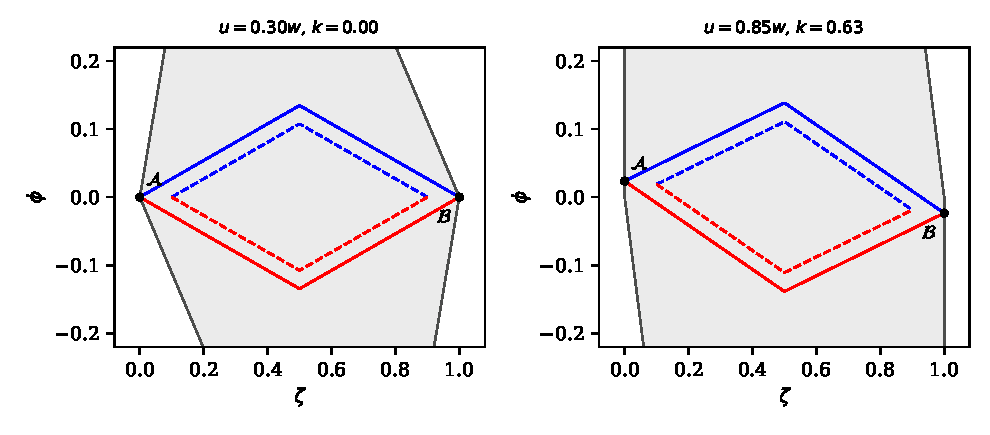
\includegraphics[width=\textwidth]{figures/fig_window.pdf}
\caption{Rescaled windows (grey, partly shown) and ideal loops for the typical car: upper branch (forward S-curve) in blue, lower branch (reverse S-curve) in red.
Solid: $\lambda=1$; dashed: $\lambda=0.8$.
Left: $u=0.3w$, untilted loop.
Right: $u=0.85w$; the window is slanted and the optimal loop is tilted by $\varpi(u)$.}
\label{fig:window}
\end{figure}

\subsection{Calibration}
Write $s_\pm(k)=1/(R\pm k)$ and
\[
  r_k=\frac{s_+(k)+s_-(k)}8=\frac{R}{4(R^2-k^2)},\qquad G_k(q)=(\xi-\tfrac12)\phi+\tfrac k2\phi^2 .
\]
Note that $r_*(u)=r_{k(u)}$ with $k(u)=\max(0,u-\tfrac w2)$.

\begin{lemma}[calibration]\label{lem:calib}
There is a constant $B$ (depending on $\delta$ and the parameters) such that, after decreasing $g_0$ if necessary, the following holds for $0<g\le g_0$ and $k\in[0,w/2]$.
Let $q$ be a manoeuvre, or a sub-interval of one, along which $|\psi|<cg$ and $\zeta_k\in[-Ag,1+Ag]$.
Then
\[
  \Delta u\ \le\ g^2\big(r_k+\Delta G_k\big)+Bg^3 ,
\]
where $\Delta$ denotes the increment from start to end.
\end{lemma}

\begin{proof}
By \eqref{eq:lift}, $\Delta u=g^2\int\phi\,\dd\xi+g^2\int(\tfrac{\tan\psi}{\psi}-1)\phi\,\dd\xi$.
Here $\xi=\zeta_k-k\phi$ is monotone along a manoeuvre with total variation at most $1+2Ag+wc$, and the second integrand is $O(g^2)$; so the second term is $O(g^4)$.
For the main term, $\dd\xi=\dd\zeta_k-k\,\dd\phi$, so
\[
  \int\phi\,\dd\xi=\Delta\Big[(\zeta_k-\tfrac12)\phi-\tfrac k2\phi^2\Big]-\int(\zeta_k-\tfrac12)\,\dd\phi=\Delta G_k-\int(\zeta_k-\tfrac12)\,\dd\phi .
\]
Along the manoeuvre, $\frac{\dd\zeta_k}{\dd s}=(d\cos\psi+k\psi')/g$, which has the sign of $d$ because $k|\psi'|\le w/(2R)<\cos\psi$ for small $g$.
So $\zeta_k$ is monotone, and $\dd\phi=\sigma\,\dd\zeta_k$ with
\[
  \sigma=\frac{\psi'}{d\cos\psi+k\psi'}\in\Big[-\frac1{R\cos\psi-k},\ \frac1{R\cos\psi+k}\Big].
\]
For reverse manoeuvres put $t=-\psi'$; the map $t\mapsto t/(\cos\psi+kt)$ is increasing.
Write $s'_\pm$ for the supremum of $1/(R\cos\psi\pm k)$ over the manoeuvre; then $s'_\pm=s_\pm(1+O(g^2))$.

For a forward manoeuvre ($\dd\zeta_k>0$) the integrand $-(\zeta_k-\frac12)\sigma$ is at most $s'_+(\frac12-\zeta_k)^+ + s'_-(\zeta_k-\frac12)^+$.
For a reverse manoeuvre we write $-\int(\zeta_k-\frac12)\sigma\,\dd\zeta_k=\int(\zeta_k-\frac12)\sigma\,|\dd\zeta_k|$.
Its integrand is at most $s'_+(\zeta_k-\frac12)^+ + s'_-(\frac12-\zeta_k)^+$.
In both cases $\zeta_k$ sweeps a sub-interval of $[-Ag,1+Ag]$ once.
Hence
\[
  -\int(\zeta_k-\tfrac12)\,\dd\phi\ \le\ (s'_++s'_-)\int_{-Ag}^{1/2}(\tfrac12-z)\,\dd z\ =\ \frac{(1+2Ag)^2}8\,(s'_++s'_-)=r_k+O(g).\qedhere
\]
\end{proof}

The bound is sharp, and $\sigma=\kappa/(\cos\psi+k\kappa)$ depends only on the steering.
In a forward manoeuvre equality requires $\sigma=s_+$ (full left lock) while $\zeta_k<\frac12$ and $\sigma=-s_-$ (full right lock) afterwards.
In a reverse manoeuvre, where $\zeta_k$ decreases, it requires $\sigma=s_+$ (full left lock) while $\zeta_k>\frac12$ and $\sigma=-s_-$ (full right lock) afterwards.
Each manoeuvre must also sweep the whole window.
This is exactly the S-curve of the construction in \cref{sec:construction}.

\subsection{The lower bound}

\begin{proposition}\label{prop:asym-lower}
$\liminf_{g\downarrow0}g^2N(g)\ge K^2$.
\end{proposition}

\begin{proof}
Fix $\delta\in(0,w/4]$ and $0<g\le g_0(\delta)$, and consider an exit motion with $N$ manoeuvres (\cref{lem:reversal}).
By \cref{lem:confine}, $|\psi|<cg$ on $[0,T_\delta]$.
A parked configuration with $|\psi|<cg$ has $u\le0$: its highest point is at most $H$, and for small $|\psi|$ this forces $u\le\frac w2(1-\cos\psi)-\max(b\sin\psi,-d_b\sin\psi)\le0$.
Let $t_0=\sup\{t\le T_\delta:\ u(t)\le0\}$.
Then $u(t_0)=0$, $0<u\le w-\delta$ on $(t_0,T_\delta]$ and $u(T_\delta)=w-\delta$.

Cut $[t_0,T_\delta]$ into the pieces $I_1,\dots,I_M$ in which it meets the manoeuvres, so $M\le N$.
On $I_j$ the variable $\xi$ is monotone with range at most $1+2Ag+wc$, so by \eqref{eq:lift} the oscillation of $u$ on $I_j$ is at most $Dg^2$ for a constant $D$ (depending on $\delta$).
Put $k_j=\max\big(0,\max_{I_j}u-\tfrac w2\big)\in[0,\tfrac w2-\delta]$.
Then $k_j\ge u-\frac w2$ on $I_j$, so \cref{lem:windows,lem:calib} give
\[
  \Delta_ju\ \le\ g^2\big(r_{k_j}+\Delta_jG_{k_j}\big)+Bg^3 .
\]

Let $F(u)=\int_0^u\dd v/r_*(v)$.
The function $1/r_*=4(R^2-k(u)^2)/R$ is Lipschitz with constant $4w/R$, and on $I_j$ it differs from $1/r_{k_j}$ by at most $(4w/R)Dg^2$.
Hence $F(u_{\rm end})-F(u_{\rm start})\le\Delta_ju/r_{k_j}+(4w/R)D^2g^4$ on every piece.
Using $1/r_{k}\le4R$ we obtain
\[
  F(w-\delta)=\sum_j\big(F(u_{\rm end})-F(u_{\rm start})\big)\ \le\ Mg^2+g^2\sum_j\frac{\Delta_jG_{k_j}}{r_{k_j}}+M\big(4RBg^3+(4w/R)D^2g^4\big).
\]

For the middle sum write $\mathcal H_j=G_{k_j}/r_{k_j}$, and recall that consecutive pieces share their endpoints.
Then
\[
  \sum_j\Delta_j\mathcal H_j=\mathcal H_M(q_{\rm end})-\mathcal H_1(q_{\rm start})+\sum_{j<M}\big(\mathcal H_j-\mathcal H_{j+1}\big)(q_{j+1,\rm start}).
\]
On the bounded set $\{|\phi|<c,\ -Ag-\frac{wc}2\le\xi\le1+Ag+\frac{wc}2\}$, which contains all states on $[t_0,T_\delta]$, the functions $G_k/r_k$ are bounded by a constant $\hat H$ and are Lipschitz in $k$ with constant $E$ (both depending on $\delta$).
Moreover $|k_j-k_{j+1}|\le2Dg^2$.
Hence $\sum_j\Delta_j\mathcal H_j\le2\hat H+2EDg^2M$.
Altogether
\[
  F(w-\delta)\ \le\ Mg^2\big(1+O(g)\big)+2\hat Hg^2,
\]
so $\liminf_{g\to0}g^2N(g)\ge F(w-\delta)$.
Letting $\delta\to0$ gives $\liminf g^2N(g)\ge F(w)=K^2$.
\end{proof}

\subsection{The construction: tilted S-curves}\label{sec:construction}

For $u\ge0$ let $k(u)=\min\big(\max(0,u-\tfrac w2),\tfrac w2\big)$, $s_\pm=s_\pm(k(u))$, and define the \emph{tilt}
\[
  \varpi(u)=\frac{s_--s_+}2=\frac{k}{R^2-k^2}.
\]
Fix $\lambda\in(0,1)$.
The \emph{ideal loop} at height $u$ is the closed curve in the $(\zeta,\phi)$-plane, $\zeta=\zeta_{k(u)}$, through the cusps
\[
  \mathcal A_u=\Big(\frac{1-\lambda}2,\ \frac{\lambda\varpi}2\Big),\qquad \mathcal B_u=\Big(\frac{1+\lambda}2,\ -\frac{\lambda\varpi}2\Big).
\]
Its upper branch runs from $\mathcal A_u$ with slope $s_+$ and then with slope $-s_-$ to $\mathcal B_u$.
Its lower branch runs from $\mathcal A_u$ with slope $-s_-$ and then with slope $s_+$ to $\mathcal B_u$.

\begin{lemma}\label{lem:loop}
The ideal loop has area $2\lambda^2r_*(u)$.
It lies in the homothetic image $\lambda\Pi_u$ of the window of \cref{rem:parallelogram} under the homothety of ratio $\lambda$ about $(\frac12,0)$, hence at distance at least $(1-\lambda)\varrho_0$ from $\partial\Pi_u$.
Here $\varrho_0>0$ does not depend on $u\in[0,w]$.
\end{lemma}

\begin{proof}
For $\lambda=1$ the loop is the parallelogram with vertices $\mathcal A_u=(0,\frac\varpi2)$, $\mathcal B_u=(1,-\frac\varpi2)$ and the turning points $\mathcal U=(\frac12,\frac{s_++s_-}4)$, $\mathcal D=(\frac12,-\frac{s_++s_-}4)$.
(With $\varpi=(s_--s_+)/2$ both turning points have abscissa $\frac12$.)
Its area is $\frac12\cdot1\cdot\frac{s_++s_-}2=\frac{s_++s_-}4=2r_*(u)$.
For general $\lambda$ the loop is the image under the homothety of ratio $\lambda$ about $(\frac12,0)$, so the area scales by $\lambda^2$.

Next we check that the four vertices lie in the convex set $\Pi_u$; then so does the whole loop.
For $u\le w/2$ (so $k=0$, $\varpi=0$) the vertices are $(0,0)$, $(1,0)$, $(\frac12,\pm\frac1{2R})$.
They satisfy $\frac w2|\phi|\le\xi\le1-\frac w2|\phi|$ because $\frac w{4R}<\frac12$, and this rhombus, with vertices $(0,0)$, $(1,0)$, $(\frac12,\pm\frac1w)$, is contained in $\Pi_u$.
For $u\ge w/2$, with $k=u-\frac w2\in[0,\frac w2]$ and $w-u=\frac w2-k$:
\begin{itemize}[nosep]
\item $\mathcal A_u$ and $\mathcal B_u$ lie on the sides $\zeta=0,1$, and they satisfy $0\le\zeta+(w-u)\phi\le1$ because $(w-u)\frac\varpi2\le1$.
The latter is equivalent to $k(\frac w2-k)\le2(R^2-k^2)$, i.e.\ to $k^2+\frac{kw}2\le2R^2$, which holds since $k^2+\frac{kw}2\le\frac{w^2}2<2R^2$ for $k\le\frac w2<R$.
\item $\mathcal U$ and $\mathcal D$ satisfy $0\le\frac12\pm(w-u)\frac{s_++s_-}4\le1$ because $(w-u)(s_++s_-)\le2$.
This is equivalent to $(\frac w2-k)R\le R^2-k^2=(R-k)(R+k)$, which holds since $\frac w2-k\le R-k$ and $R\le R+k$.
\end{itemize}
Finally, $\Pi_u$ contains a disk of radius $\varrho_0>0$ about $(\frac12,0)$, with $\varrho_0$ independent of $u\in[0,w]$ (its sides stay at distance bounded below from that point).
The homothety therefore maps $\Pi_u$ into the set of points at distance at least $(1-\lambda)\varrho_0$ from $\partial\Pi_u$.
\end{proof}

The ideal loop is realised by two manoeuvres, each consisting of two full-lock arcs (an S-curve).
\begin{itemize}[nosep]
\item Forward: full left lock, then full right lock; this follows the upper branch from $\mathcal A_u$ to $\mathcal B_u$.
\item Reverse: full left lock, then full right lock; in reverse the heading first decreases and then increases, so this follows the lower branch back to $\mathcal A_{u'}$, where $u'$ is the new height.
\end{itemize}
Explicitly, a forward S-curve from heading $\psi_A$ to heading $\psi_B$ with horizontal displacement $\Delta x$ has its apex heading $\psi_{\rm top}$ given by $2\sin\psi_{\rm top}=\Delta x/R+\sin\psi_A+\sin\psi_B$.
It lifts the car by $R\big(\cos\psi_A+\cos\psi_B-2\cos\psi_{\rm top}\big)$.
The reverse S-curve is analogous, with apex heading $\psi_{\rm bot}$.

\begin{proposition}\label{prop:asym-upper}
$\limsup_{g\downarrow0}g^2N(g)\le K^2$.
\end{proposition}

\begin{proof}
Fix $\lambda\in(0,1)$.
Start from the parked level configuration $q_0=\big((d_b+g\frac{1-\lambda}2,\ m+\frac w2),0\big)$, at height $u=0$ with $(\zeta,\phi)=\mathcal A_0$.
Repeat \emph{cycles}: from the configuration corresponding to $\mathcal A_u$ at height $u$, drive the forward S-curve to the configuration corresponding to $\mathcal B_u$.
Then drive the reverse S-curve to the configuration corresponding to $\mathcal A_{u_1}$, where $u_1$ is the height reached after the forward S-curve; the reverse S-curve changes the height only by $O(g^2)$.

\emph{Feasibility.}
In rescaled coordinates the arcs of an S-curve have slope $\dd\phi/\dd\zeta=s_+(1+O(g^2))$ and $-s_-(1+O(g^2))$.
The S-curve is determined by its end points through the explicit formula for its apex heading above, which depends continuously on the data. Its rescaled trace consists of two curves of slopes $s_+(1+O(g^2))$ and $-s_-(1+O(g^2))$ joining the same end points as the two segments of the ideal branch, so the turning points differ by $O(g^2)$ and the trace lies within $O(g^2)$ of the ideal branch, uniformly in $u$. The reverse S-curve is aimed at the cusp $\mathcal A_{u_1}$; since $|u_1-u|=O(g^2)$, this differs from $\mathcal A_u$ by $O(g^2)$, which the same estimates absorb.
Next we need \emph{sufficient} conditions for freeness.
Here $c$ denotes a constant larger than the largest $|\phi|$ on the loops, $(s_++s_-)/4$ (it is not the constant of \cref{lem:confine}).
Let $|\psi|<cg$ and $u\ge A''g$, where $A''=2c(b+d_b)$.
Then no point of the car lies at height $\le m$, and the curb is no issue.
The part of the footprint inside the band $(m,H)$ has its leftmost and rightmost points among the corners and the points where the front and rear edges cross the line $y=H$.
Hence $q$ is free if, for $\psi\ge0$,
\begin{align*}
  P_x&\ge d_b\sec\psi+(\tfrac w2-u)\tan\psi &&\text{if }\cRL_y\ge H,\\
  P_x&\ge d_b\cos\psi+\tfrac w2\sin\psi &&\text{if }\cRL_y<H,\\
  P_x&\le L-b\cos\psi-\tfrac w2\sin\psi ,
\end{align*}
and symmetrically for $\psi<0$.
The last condition is still sufficient when $\cFC$ lies above $H$, since the band part then ends at the crossing of the curb-side edge with $y=H$, to the left of $\cFC$.
For $u\ge A''g$ the corner $\cRL$ (for $\psi\ge0$) or $\cFL$ (for $\psi<0$) lies above $H$.
So, in rescaled coordinates and up to $O(g)$, these conditions are exactly the constraints defining $\Pi_u$; for $u<w/2$ we use $k=0$ and the second parallelogram of \cref{rem:parallelogram}.
Thus the set of free rescaled states contains $\{(\zeta,\phi):\mathrm{dist}((\zeta,\phi),\R^2\setminus\Pi_u)\ge A'g\}$ for a constant $A'$.
For $0\le u<A''g$ we use instead the conservative sufficient condition that the whole footprint lies in $\{0\le x\le L\}$; the curb is again no issue, because the lowest point is at height at least $m-O(g)>0$.
In rescaled coordinates this reads $\tfrac w2|\phi|+O(g)\le\xi\le1-\tfrac w2|\phi|-O(g)$, and the untilted loop satisfies it with margin $\frac{1-\lambda}2(1-\frac w{2R})$.
By \cref{lem:loop} all cycles are therefore free once $g$ is small enough (depending on $\lambda$).

\emph{Lift per cycle.}
By \eqref{eq:lift}, the lift of a manoeuvre is $g^2\big(\int\phi\,\dd\xi+O(g^2)\big)$.
Over a cycle this is $g^2$ times the area enclosed by the rescaled trace in the $(\xi,\phi)$-plane, which equals the area in the $(\zeta,\phi)$-plane because the shear preserves area.
On each full-lock arc the slope $\dd\phi/\dd\zeta$ equals $s_\pm(1+O(g^2))$, so the trace of a cycle lies within $O(g^2)$ of the ideal loop.
The trace of a cycle is not exactly closed, since it ends at $\mathcal A_{u_1}$ rather than at $\mathcal A_u$, and the sheared coordinate changes from $\zeta_{k(u)}$ to $\zeta_{k(u_1)}$; both gaps are $O(g^2)$, and closing them changes the enclosed area by $O(g^2)$.
Hence a cycle lifts the car by $g^2\big(2\lambda^2r_*(u)+O(g)\big)$.
(Explicitly, a forward S-curve lifts by $R(\cos\psi_A-\cos\psi_{\rm top})+R(\cos\psi_B-\cos\psi_{\rm top})$, whose leading term $\frac R2g^2(2\phi_{\rm top}^2-\phi_A^2-\phi_B^2)$ is the area under the upper branch.)

\emph{Counting.}
The number of cycles until $u\ge w$ is therefore at most
\[
  \int_0^w\frac{\dd u}{2\lambda^2r_*(u)g^2}\,(1+O(g))+1=\frac{K^2}{2\lambda^2g^2}(1+O(g))+1 .
\]
After that, $O(1/g)$ further cycles (with $k=w/2$) lift the lowest point of the car above $H$; for $u\ge w$ the constraints only weaken, so the window contains $\{0\le\zeta_{w/2}\le1\}$ and the loop with $k=w/2$ stays free.
One last manoeuvre in the free lane makes the car parallel.
Hence $N(g)\le K^2/(\lambda^2g^2)(1+O(g))+O(1/g)$.
Then $\limsup g^2N(g)\le K^2/\lambda^2$, and $\lambda\uparrow1$ concludes.
\end{proof}

\begin{remark}
Replacing the tilted loops by untilted diamonds (tilt $0$ at all heights) gives the simpler \emph{plain crawl}.
It achieves $\limsup g^2N(g)\le4Rw$, only a factor $\sqrt{1-w^2/(24R^2)}\approx0.995$ (for the typical car) away from the optimal $K$.
Simulations of both crawls with exact collision checks agree with the predictions (\cref{tab:crawl,fig:crawl}).
\end{remark}

\begin{table}[ht]
\centering
\begin{tabular}{lccccc}
\toprule
$g$ [m] & 0.4 & 0.2 & 0.1 & 0.05 & 0.025\\
\midrule
plain crawl, $g^2N$ & 23.52 & 24.44 & 25.41 & 26.07 & 26.40\\
tilted crawl, $g^2N$ & 23.84 & 23.96 & 25.07 & 25.77 & 26.12\\
\bottomrule
\end{tabular}
\caption{Simulated crawls for the typical car (each manoeuvre chosen maximal, collision checks exact up to sampling).
The limits predicted by the theory are $4Rw=26.73$ for the plain crawl and $K^2=26.47$ for the tilted crawl; in both cases the error is roughly proportional to $g$.}
\label{tab:crawl}
\end{table}

\begin{figure}[ht]
\centering
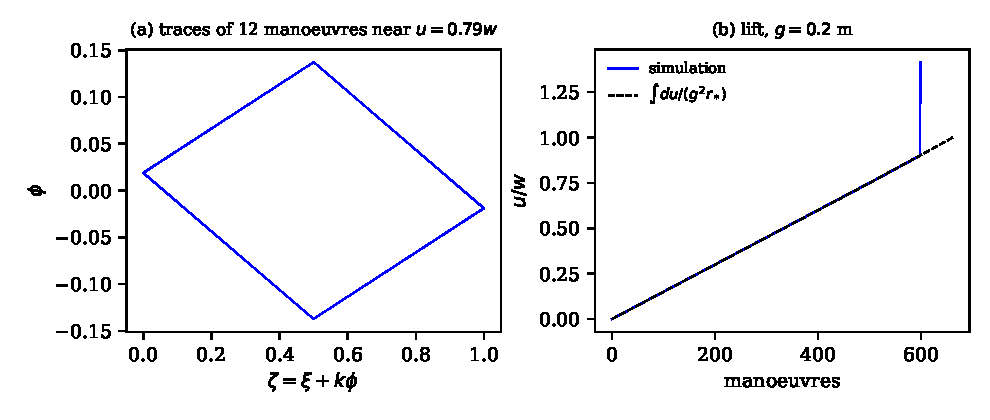
\includegraphics[width=\textwidth]{figures/fig_crawl.pdf}
\caption{The tilted crawl simulated with exact geometry, typical car, $g=0.2$ m.
(a) Rescaled traces of twelve consecutive manoeuvres near $u=0.79w$; they follow the $\lambda=1$ tilted loop at that height (cf.\ \cref{fig:window}).
(b) The lift $u$ against the number of manoeuvres, compared with the prediction $\int_0^u\dd v/(g^2r_*(v))$.
The final jump is the escape, once large tilts become admissible near the top.}
\label{fig:crawl}
\end{figure}

\subsection{Proofs of \texorpdfstring{\cref{thm:mono,thm:asym}}{Theorems}}\label{sec:asym-proofs}

\begin{proof}[Proof of \cref{thm:asym}]
\Cref{prop:asym-lower,prop:asym-upper} give $g^2N(g)\to K^2$.
For the equivalent statement let $\varepsilon\in(0,K^2)$.
For $g\le g_\varepsilon$ we have $(K^2-\varepsilon)/g^2\le N(g)\le(K^2+\varepsilon)/g^2$.
Since $\Lmin(n)-\ell=\inf\{g:N(g)\le n\}$, for $n$ large this gives $\sqrt{(K^2-\varepsilon)/n}\le\Lmin(n)-\ell\le\sqrt{(K^2+\varepsilon)/n}$.
Finally, $K^2=2Rw+\frac4R\int_0^{w/2}(R^2-t^2)\dd t=4Rw-\frac{w^3}{6R}$.
\end{proof}

\begin{proof}[Proof of \cref{thm:mono}]
Monotonicity is \cref{lem:monoL}.
By \cref{prop:asym-lower} there is $g_1>0$ with $N(g)\ge K^2/(2g^2)$ for $g\le g_1$.
So for each $n$, $N(g)>n$ for all $g<\min(g_1,K/\sqrt{2n})$, i.e.\ $\Lmin(n)\ge\ell+\min(g_1,K/\sqrt{2n})>\ell$.
By \cref{prop:asym-upper}, $N(g)<\infty$ for small $g$, so $\Lmin(n)\to\ell$.
\end{proof}

\section{The soft curb}\label{sec:soft}

In this section ``free'', ``parked'' and ``lane configuration'' refer to the soft-curb model of \cref{sec:model-soft}.
The curb now constrains only the tyres.
Two tyre points matter: the outer rear corner of the curb-side rear tyre and the outer front corner of the curb-side front tyre,
\[
  \cTr=P-\lambda\,\e-T_o\,\n,\qquad \cTf=P+a\,\e-T_o\,\n,\qquad a:=d_w+\lambda .
\]
For $\psi\in[0,\pi/2]$ the lowest point of $\W(q)$ is $\cTr$, and for $\psi\in[-\pi/2,0]$ it is $\cTf$.
In analogy with $r$ and $\beta$ we put
\[
  r_t=\sqrt{\lambda^2+(R+T_o)^2},\qquad (\cos\beta_t,\sin\beta_t)=\frac{(R+T_o,\lambda)}{r_t},
\]
so that $\cTr=C+r_t\,\e(\psi-\tfrac\pi2-\beta_t)$ and $\cTr_y=C_y-r_t\cos(\psi-\beta_t)$.

\subsection{Parked cars}
If $H<\min(b+\lambda,\,d_b+a)$, let $\psi_t$ and $\psi_t'$ be the roots in $(0,\pi/2)$ of
\[
  (b+\lambda)\sin\psi+(w-\delta_s)\cos\psi=H\qquad\text{and}\qquad(d_b+a)\sin\psi+(w-\delta_s)\cos\psi=H ,
\]
respectively, and put $\psi_{\max}=\max(\psi_t,\psi_t')$.
The roots are unique, because each left side increases from $w-\delta_s<H$ and then decreases to $b+\lambda>H$, respectively $d_b+a>H$.

\begin{lemma}[parked cars, soft curb]\label{lem:soft-fit}
Assume $H<\min(b+\lambda,\,d_b+a)$.
If $q$ is parked, then modulo $2\pi$ either $\psi\in[-\psi_t',\psi_t]$ or $\psi\in[\pi-\psi_t,\pi+\psi_t']$.
Assume moreover
\begin{equation}\label{eq:soft-band}
  (w-\delta_s)\cos\psi_{\max}-\max(d_b,d_f)\sin\psi_{\max}>m ,
\end{equation}
and let $q$ be parked with $\psi\in[-\psi_t',\psi_t]$.
\begin{enumerate}[label=(\alph*)]
\item If $\psi\ge0$, then $C_x\ge X(\psi)$ and $r_t\cos(\psi-\beta_t)\le C_y\le H+Y(\psi)$.
\item If $\psi<0$, then $C_x\ge d_b\cos\psi+\Rm|\sin\psi|$, $C'_x\ge d_b\cos\psi-\Rp|\sin\psi|$ and $r_t\cos(\psi-\beta_t)\le C_y\le H+\Rm\cos\psi-d_b|\sin\psi|$.
\item $\cFL_x\le L$.
\end{enumerate}
\end{lemma}

\begin{proof}
For $\psi\in[0,\pi/2]$ the lowest point of $\W(q)$ is $\cTr$ and the highest point of $\fp(q)$ is $\cFL$.
Since $\cFL-\cTr=(b+\lambda)\e+(w-\delta_s)\n$, the conditions $\cTr_y\ge0$ and $\cFL_y\le H$ give $(b+\lambda)\sin\psi+(w-\delta_s)\cos\psi\le H$, hence $\psi\le\psi_t$.
For $\psi\in[-\pi/2,0]$ the same argument with $\cTf$ and $\cRL$, where $\cRL-\cTf=-(d_b+a)\e+(w-\delta_s)\n$, gives $|\psi|\le\psi_t'$.
For the other headings the two sides of the car exchange their roles: then the lowest tyre point is a corner of a lane-side tyre and the highest body point is a curb-side corner.
The same computation gives $\psi\in[\pi-\psi_t,\pi+\psi_t']$.

(a) We have $\cTr_y\ge0$ and $\cFL_y\le H$.
Moreover $\cRL_y=\cTr_y+(w-\delta_s)\cos\psi-(d_b-\lambda)\sin\psi>m$ by \eqref{eq:soft-band}.
So $\cRL$ lies in the band or on its upper boundary, and as in \cref{lem:parked} we get $\cRL_x\ge0$, i.e.\ $C_x\ge X(\psi)$.
The upper bound for $C_y$ comes from $\cFL_y\le H$ and the lower bound from $\cTr_y\ge0$.
(b) Now $\cRL$ is the highest point, and $\cRL_y=\cTf_y+(d_b+a)|\sin\psi|+(w-\delta_s)\cos\psi>m$.
So again $\cRL_x\ge0$, and the bounds follow as in \cref{lem:parked}(b) and (a).
(c) We have $\cFL_y\le H$.
For $\psi\ge0$, $\cFL_y=\cTr_y+(b+\lambda)\sin\psi+(w-\delta_s)\cos\psi>m$.
For $\psi<0$, the identity $\cFL-\cTf=(d_f-\lambda)\e+(w-\delta_s)\n$ and \eqref{eq:soft-band} give $\cFL_y>m$.
Hence $\cFL$ lies in the band or on its upper boundary, and $\cFL_x\le L$ by continuity.
\end{proof}

By \cref{lem:mirror} we may assume that an exit starts at a parked configuration with $\psi\in[-\psi_t',\psi_t]$.

\subsection{One manoeuvre}
The optimal exit has the shape of the one in \cref{thm:one}, but it starts from a more strongly tilted position.
The tilt is now limited by the rear tyre touching the curb at rest, rather than by the swing of the rear corner during the exit.
Define $\psi_b^{\rm s},\psi_n^{\rm s}\in(0,\pi/2)$ and $\eta$ by
\[
  \sin\psi_b^{\rm s}=\frac{H+\delta_s}{b+\lambda},\qquad \sin\psi_n^{\rm s}=\frac{H+\delta_s}{a},\qquad \eta=(d_f-\lambda)\sin\gamma+\delta_s ,
\]
and let $\psi_u^{\rm s}\in(0,\pi/2)$ solve $(R-T_o)(1-\cos\psi_u^{\rm s})+\lambda\sin\psi_u^{\rm s}=H+\delta_s$.
Put
\[
  h_0=H-(w-\delta_s)\cos\psi_{\max},\qquad h_1=\frac{Ha}{a+d_b},\qquad \Gamma(z)=\sqrt{a^2-z^2}-a\log\frac{a+\sqrt{a^2-z^2}}{z},
\]
and, with $f_b(\psi)=d_b\cos\psi-\tfrac w2\sin\psi$ as in \eqref{eq:Bback},
\begin{equation}\label{eq:Bback-soft}
  B^{\rm s}_{\rm back}=b\cos\psi_{\max}-\tfrac w2\sin\psi_{\max}+\min\big(f_b(-\psi_n^{\rm s}),f_b(\psi_u^{\rm s})\big)+\frac{R}{R+T_o}\big(\Gamma(h_1)-\Gamma(h_0)\big).
\end{equation}
Finally let
\[
  \varphi_0(\psi)=X(\psi)+\sqrt{\rho^2-Y(\psi)^2},
\]
which is the function $\varphi_{\rm c}$ of the proof of \cref{prop:one-forward} without its curb-cost term.

\begin{assumption}\label{ass:soft}
\leavevmode
\begin{enumerate}[label=(S\arabic*),nosep]
\item\label{S:db} $d_b<b$ and $\lambda\le\min(d_b,d_f)$;
\item\label{S:fit} $H+\delta_s<\min(b+\lambda,\,d_b+a,\,\lambda+R-T_o)$, $\psi_{\max}<\gamma$, \eqref{eq:soft-band}, $(w-\delta_s)\cos\psi_b^{\rm s}>m$, $\Rp\cos\psi_t>\Rm$, $\Rm\ge d_b\tan(\psi_t'/2)$, $\Rm\tan\psi_t'<b$, $r_t\cos(\psi_{\max}+\beta_t)\ge H$ and $h_0<h_1$;
\item\label{S:nose} $2Rb>w\rho$, $m\rho+(d_f-\lambda)\Rp<(w-\delta_s)b$ and $b\rho>(H+\eta)\Rp$;
\item\label{S:swing} $\lambda\le\big(H+Y(\psi_t)\big)\sin\psi_t$;
\item\label{S:min} $\cos\psi_t\sqrt{b^2+2Rw}>\Rm\sin\psi_t+b$;
\item\label{S:end} $Y(\psi_t)\ge d_b$;
\item\label{S:far} $d_b\cos\psi_{\max}-\Rp\sin\psi_{\max}+\rho\ge\Lambda_1^{\rm s}$ and $B^{\rm s}_{\rm back}\ge\Lambda_1^{\rm s}$, where $\Lambda_1^{\rm s}=\varphi_0(\psi_t)$ as in \eqref{eq:Lam1soft} below.
\end{enumerate}
\end{assumption}

These conditions are checked by the script \texttt{numerics/soft\_theory.py}.
They hold for the typical car, and for the compact car, the mid-size sedan, the large SUV and the van of \cref{tab:cars}.
For the city car only \ref{S:swing} fails, by a narrow margin (see below).

\begin{theorem}[one manoeuvre, soft curb]\label{thm:one-soft}
Under \cref{ass:soft},
\begin{equation}\label{eq:Lam1soft}
  \Lmins(1)=\Lambda_1^{\rm s}:=\varphi_0(\psi_t)=X(\psi_t)+\sqrt{\rho^2-Y(\psi_t)^2}.
\end{equation}
An optimal exit starts from the parked configuration $q_t$ with heading $\psi_t$, $\cFL_y=H$ and $\cRL_x=0$, whose rear tyre touches the curb ($\cTr_y=0$).
It drives forward with full left lock, during which its front curb-side corner grazes $\Qf$, and then straightens with full right lock.
\end{theorem}

In the same notation, \cref{thm:one} says $\Lmin(1)=\varphi_0(\psi_d)$.
The two optimal exits differ only in the tilt of the starting position.
Since $\varphi_0$ is decreasing on the relevant range, the larger tilt gives the shorter slot.
For the typical car $\psi_t=0.0561$ rad $=3.21^\circ$, against $\psi_d=1.80^\circ$, and $\Lambda_1^{\rm s}=5.809$ m, against $\Lambda_1=5.833$ m.
In the optimal position the rear curb-side corner overhangs the curb by $5.8$ cm.
Further $\psi_t'=0.0577$, $\beta_t=0.0545$, $\psi_b^{\rm s}=0.565$, $\psi_n^{\rm s}=0.782$, $\psi_u^{\rm s}=1.187$ and $B^{\rm s}_{\rm back}=7.34$ m.
For the city car, during the exit from $q_t$ the outer rear corner of the tyre would dip $0.025$ mm below the curb.
There the numerical optimum, $4.89485$ m, exceeds $\varphi_0(\psi_t)=4.89480$ m by less than $0.1$ mm.

\begin{proof}
We follow \cref{sec:one} and list the changes.
By \cref{lem:mirror,lem:soft-fit} we may assume that an exit starts with $\psi(0)\in[-\psi_t',\psi_t]$.

\emph{Upper bound.}
Let $L=\Lambda_1^{\rm s}$ and $q_t=(P,\psi_t)$ with $P=(d_b\cos\psi_t+\tfrac w2\sin\psi_t,\ H-b\sin\psi_t-\tfrac w2\cos\psi_t)$.
Then $\cFL_y=H$ and $\cRL_x=0$.
By the definition of $\psi_t$, $\cTr_y=\cFL_y-(b+\lambda)\sin\psi_t-(w-\delta_s)\cos\psi_t=0$.
The left centre is $C=(X(\psi_t),\,H+Y(\psi_t))$, and $\Qf$ lies on the circle of radius $\rho$ about $C$.
The proof of \cref{prop:one-upper} applies with the following changes.
\begin{itemize}[nosep]
\item The configuration $q_t$ is parked.
Its lowest tyre point $\cTr$ is on the curb, and the footprint lies in $\{y\le H\}\cap\{x\ge0\}$ with $\cFC_x<L$, exactly as there.
\item During the first arc no point of the footprint enters $\Or$.
All points start below $C$, because $C_y=H+Y(\psi_t)>H$ by \ref{S:end}.
A point below $C$ moves to the right and so keeps $x\ge0$; once it rises above $C$ it is in the lane.
(This argument also makes the condition $X(\psi_d)\ge0$ in \cref{prop:one-upper} unnecessary.)
\item For the tyres, a point with body coordinates $(u,v)$ descends during the arc only while $\tan\psi<-u/(R-v)$.
For $\psi\ge\psi_t$ this requires $u<0$ and $R-v<\lambda/\tan\psi_t$, so the point is at distance less than $\lambda/\sin\psi_t$ from $C$.
Its height therefore stays above $C_y-\lambda/\sin\psi_t\ge0$ by \ref{S:swing}; all other tyre points rise.
\item At heading $\pi/2$ a body point $(u,v)$ is at height $C_y+u\ge H+Y(\psi_t)-d_b\ge H$ by \ref{S:end}.
\end{itemize}
The second arc is as in \cref{prop:one-upper}.

\emph{Forward exits.}
Let a forward manoeuvre lead from a parked configuration $q_0$ with $\psi(0)\in[-\psi_t',\psi_t]$ to a lane configuration, and suppose $L<\Lambda_1^{\rm s}$.
Steps 1--7 of the proof of \cref{prop:one-forward} go through with the following changes.
The curb enters there only through lower bounds for the heights of points.
\begin{itemize}[nosep]
\item Step 2(i): from $\cTr_y\ge0$ and $\cFC-\cTr=(b+\lambda)\e-\delta_s\n$ we get $\cFC_y\ge(b+\lambda)\sin\psi-\delta_s$.
So for $s<\tau$ the heading satisfies $\psi<\psi_b^{\rm s}$ whenever $\psi\in[0,\pi/2]$; in (ii) and below, $\psi_b$ is replaced by $\psi_b^{\rm s}$.
In (iii), $\cRL_x(0)\ge0$ (\cref{lem:soft-fit}) gives $C'_x(0)=P_x(0)+R\sin\psi(0)\ge d_b\cos\psi(0)+\Rp\sin\psi(0)\ge d_b\cos\psi_{\max}-\Rp\sin\psi_{\max}$, and $\psi(0)>-\gamma$ by \ref{S:fit}.
\item The case $\psi(t)=-\gamma$: now $\cFL_x(t)\ge d_b\cos\psi_{\max}-\Rp\sin\psi_{\max}+\rho\ge\Lambda_1^{\rm s}>L$ by \ref{S:far}, and $\cFL_y(t)<H$ as before.
If $\cFL_y(t)\le m$, then, since $\cTf-\cFL=-(d_f-\lambda)\e-(w-\delta_s)\n$,
\[
  \cTf_y=\cFL_y+(d_f-\lambda)\sin\gamma-(w-\delta_s)\cos\gamma\le m+\frac{(d_f-\lambda)\Rp-(w-\delta_s)b}{\rho}<0
\]
by \ref{S:nose}, and the front tyre meets the curb.
\item Step 5 with $\psi\ge0$ needs $\cFL_y>m$.
This now follows from $\cFL_y=\cFC_y+w\cos\psi\ge(w-\delta_s)\cos\psi>m$ for $\psi\in[0,\psi_b^{\rm s}]$, by \ref{S:fit}.
\item Step 5 with $\psi<0$: the case $\cFL_y\le m$ is excluded as in the previous item, because $(d_f-\lambda)|\sin\psi|-(w-\delta_s)\cos\psi$ increases with $|\psi|<\gamma$.
Since $\cFC-\cTf=(d_f-\lambda)\e-\delta_s\n$, we have $\cFC_y\ge-\eta$.
So the bound $(H-\cFC_y)|\sin\psi|\le H\sin\gamma$ becomes $(H-\cFC_y)|\sin\psi|\le(H+\eta)\sin\gamma<b$, by \ref{S:nose}.
\item Of Step 7 only the first statement is needed: $|C-\Qf|$ is non-increasing on $[0,\tau]$.
\end{itemize}
Steps 8 and 9 are replaced by a simpler argument, which needs no curb cost.
By Steps 6 and 7, $|C(0)-\Qf|\ge|C(\tau)-\Qf|\ge\rho$.
By \cref{lem:soft-fit} and \ref{S:fit}, $C_y(0)\ge r_t\cos(\psi_{\max}+\beta_t)\ge H$.
Also $C_x(0)=\cFL_x-b\cos\psi(0)-\Rm\sin\psi(0)<L$, because $\Rm\tan\psi_t'<b$.
Hence
\[
  L\ \ge\ C_x(0)+\sqrt{\rho^2-(C_y(0)-H)^2},
\]
and the right side increases with $C_x(0)$ and decreases with $C_y(0)\ge H$.
If $\psi(0)\in[0,\psi_t]$, \cref{lem:soft-fit}(a) gives $L\ge\varphi_0(\psi(0))$.
If $\psi(0)<0$, \cref{lem:soft-fit}(b) gives $C_x(0)\ge d_b\cos\psi+\Rm|\sin\psi|\ge d_b$, because $\Rm\ge d_b\tan(\psi_t'/2)$, and $C_y(0)\le H+\Rm$; so $L\ge\varphi_0(0)$.
Finally, $\varphi_0$ is decreasing on $[0,\psi_t]$.
There $d_b\le Y\le\Rm$ by \ref{S:end}, and as in Step 9 the derivative is at most $-\Rm\cos\psi_t+\Rm(\Rm\sin\psi_t+b)/\sqrt{b^2+2Rw}<0$, by \ref{S:min}.
Hence $L\ge\varphi_0(\psi_t)=\Lambda_1^{\rm s}$, a contradiction.

\emph{Reverse exits.}
Let a reverse manoeuvre lead from a parked configuration with $\psi(0)\in[-\psi_t',\psi_t]$ to a lane configuration.
We show $L\ge B^{\rm s}_{\rm back}$, following \cref{prop:one-reverse} with
\[
  h=P_y-T_o\cos\psi ,
\]
the height of the outer sidewall of the curb-side rear tyre at the axle.
Now $h'=-\sin\psi\,(1-T_o\psi')$ with $1-T_o\psi'\in[1-T_o/R,\,1+T_o/R]$, so $h$ increases only while $\psi<0$.
Let $\tau_r$ be the first time with $\cRC_y=H$.
\begin{itemize}[nosep]
\item The highest point of the parked car, $\cFL$ or $\cRL$, is at height at most $H$.
Hence $h(0)\le H-(w-\delta_s)\cos\psi(0)\le h_0$.
\item On $[0,\tau_r)$ we have $h<H+\delta_s$.
While $\psi<0$ this follows from $\cRC_y=h+d_b|\sin\psi|-\delta_s\cos\psi<H$, and while $\psi\ge0$ the height $h$ does not increase.
\item If $\psi\le0$, then $\cTf_y=h-a|\sin\psi|\ge0$, so $|\sin\psi|\le h/a<\sin\psi_n^{\rm s}$.
\item The function $C'_y=h-(R-T_o)\cos\psi$ does not increase while $\psi\ge0$.
Suppose $\psi$ first reached $\psi_u^{\rm s}$ at a time $t$.
The argument of \cref{prop:one-reverse} would give $h(t)<H+\delta_s-(R-T_o)(1-\cos\psi_u^{\rm s})=\lambda\sin\psi_u^{\rm s}$; if the positive excursion starts at time $0$, it uses $\Rp\cos\psi_t>\Rm$.
This contradicts $\cTr_y=h(t)-\lambda\sin\psi_u^{\rm s}\ge0$.
\end{itemize}
Hence $\psi\in(-\psi_n^{\rm s},\psi_u^{\rm s})$ on $[0,\tau_r]$.
At $\tau_r$ we have $h(\tau_r)\ge h_1$.
Indeed, if $\psi\le0$ then $H=\cRC_y\le h+d_b|\sin\psi|\le h(1+d_b/a)$, and if $\psi>0$ then $H<h$.

The Gronwall step is replaced by a sharper estimate.
Let $g(z)=\sqrt{a^2-z^2}/z$, so that $\Gamma'=g$ on $(0,a]$.
Let $s_0$ be the last time in $[0,\tau_r]$ with $h\le h_0$; on $[s_0,\tau_r]$ we have $h_0\le h<H+\delta_s<a$.
While $\psi<0$, the bounds $h'\le(1+T_o/R)|\sin\psi|$ and $|\sin\psi|\le h/a$ give
\[
  \frac{\dd}{\dd s}\Gamma(h)=g(h)\,h'\ \le\ \frac{R+T_o}{R}\sqrt{1-\frac{h^2}{a^2}}\ \le\ \frac{R+T_o}{R}\cos\psi=-\frac{R+T_o}{R}P_x'.
\]
While $\psi\ge0$ the left side is $\le0\le-P_x'$.
Integrate over $[s_0,\tau_r]$, use that $P_x$ is non-increasing, and use $h(s_0)=h_0$ and $h(\tau_r)\ge h_1$.
This gives
\[
  P_x(0)-P_x(\tau_r)\ \ge\ \frac{R}{R+T_o}\big(\Gamma(h_1)-\Gamma(h_0)\big).
\]
As in \cref{prop:one-reverse}, $P_x(\tau_r)\ge f_b(\psi(\tau_r))\ge\min(f_b(-\psi_n^{\rm s}),f_b(\psi_u^{\rm s}))$.
By \cref{lem:soft-fit}(c), $P_x(0)\le L-b\cos\psi(0)+\tfrac w2\sin\psi(0)\le L-b\cos\psi_{\max}+\tfrac w2\sin\psi_{\max}$.
Together, $L\ge B^{\rm s}_{\rm back}\ge\Lambda_1^{\rm s}$ by \ref{S:far}.

The three parts and \cref{lem:reversal} prove the theorem.
\end{proof}

\subsection{Two manoeuvres}
With a soft curb, the textbook two-move exit becomes admissible: reverse with full right lock until the rear bumper touches the car behind, then leave with full left lock.
Let $\alpha_s\in(0,\pi/2)$ be the solution of
\[
  \Rp\cos\alpha_s-b\sin\alpha_s=R,\qquad\text{i.e.}\quad \alpha_s=\arccos(R/\rho)-\arctan(b/\Rp),
\]
and put
\[
  \Lambda_2^{\rm s}=b+d_b\cos\alpha_s+\Rp\sin\alpha_s .
\]

\begin{proposition}\label{prop:two-soft}
Assume
\begin{enumerate}[label=(T\arabic*),nosep]
\item\label{T:db} $d_b<b$ and $b\tan\alpha_s<\Rm$;
\item\label{T:tyre} $m+\tfrac w2-R+(R-T_o)\cos\alpha_s-\lambda\sin\alpha_s\ge0$;
\item\label{T:end} $2R\cos\alpha_s-\Rp\ge d_b$ and $\lambda\le(H+2R\cos\alpha_s-\Rp)\sin\alpha_s$.
\end{enumerate}
Then $\Lmins(2)\le\Lambda_2^{\rm s}$.
\end{proposition}

For the typical car $\alpha_s=0.2256$ rad $=12.9^\circ$ and $\Lambda_2^{\rm s}=5.312$ m.
In the rigid model the best two-manoeuvre exit we know needs $\Lambda_2^*=5.4104$ m (\cref{prop:two-better}).
The value $\Lambda_2^{\rm s}$ depends neither on the margin nor on the tyres; these enter only through \ref{T:tyre} and \ref{T:end}.
\Cref{fig:two-soft} shows the exit.

\begin{proof}
Let $L=\Lambda_2^{\rm s}$ and start from the level configuration $q_0=((L-b,\,m+\tfrac w2),0)$.
Its footprint is $[L-\ell,L]\times[m,H]$ with $L-\ell=\sin\alpha_s(\Rp-d_b\tan\tfrac{\alpha_s}2)>0$.
So $q_0$ is parked, and its front bumper touches the car in front.

\emph{Reverse with full right lock through the angle $\alpha_s$.}
The car rotates counter-clockwise about $C'=(L-b,\,m+\tfrac w2-R)$.
After rotating by $t\in[0,\alpha_s]$, a body point $(u,v)$ sits at $C'$ plus the vector $(u,v+R)$ rotated by $t$.
Its height above $C'$ is $u\sin t+(v+R)\cos t\ge\Rm\cos t-d_b\sin t>0$, by \ref{T:db}.
So every point stays above $C'$ and moves to the left, away from $\Of$.
The leftmost point $\cRL$ has abscissa $L-b-d_b\cos t-\Rp\sin t$, which decreases to $0$ at $t=\alpha_s$ by the definition of $L$.
Hence the car stays clear of $\Or$ and ends with its rear bumper against the car behind.
All tyre points have heights at least $m+\tfrac w2-R+(R-T_o)\cos t-\lambda\sin t$.
This decreases in $t$ and is $\ge0$ at $t=\alpha_s$ by \ref{T:tyre}.
The bodywork does pass over the curb: for the typical car $\cRC$ ends $7.0$ cm beyond it, while the tyre keeps $8.0$ cm from it.

\emph{Forward exit with full left lock.}
At heading $\alpha_s$ the left centre is
\[
  C_1=C'+2R\,\n(\alpha_s)=\big(X(\alpha_s),\,H+2R\cos\alpha_s-\Rp\big),
\]
and $|C_1-\Qf|^2=(b+2R\sin\alpha_s)^2+(2R\cos\alpha_s-\Rp)^2=\rho^2$ by the definition of $\alpha_s$.
The exit is free by the argument of the upper bound in \cref{thm:one-soft}, with $C_1$ and $\alpha_s$ in place of $C$ and $\psi_t$.
\begin{itemize}[nosep]
\item The footprint stays in the disk of radius $\rho$ about $C_1$, which misses $\Of$.
\item All points start below $C_1$: the highest point $\cFL$ lies $\Rm\cos\alpha_s-b\sin\alpha_s>0$ below it. So they move right until they rise above $C_1$, into the lane.
\item Descending tyre points stay above $C_{1,y}-\lambda/\sin\alpha_s\ge0$, by \ref{T:end}.
\item At heading $\pi/2$ the lowest point is at height $C_{1,y}-d_b\ge H$.
\end{itemize}
The final right-lock arc is as in \cref{prop:one-upper}.
\end{proof}

In driving terms, one reverses into the gap along an S-curve (right lock, then left lock) until the rear bumper touches the car behind.
The car is then turned $12.9^\circ$ nose-up.
One then pulls forward with full right lock until the car is level.
In the rigid model this is impossible: the rear curb-side corner would end $7.0$ cm inside the curb.

\begin{figure}[ht]
\centering
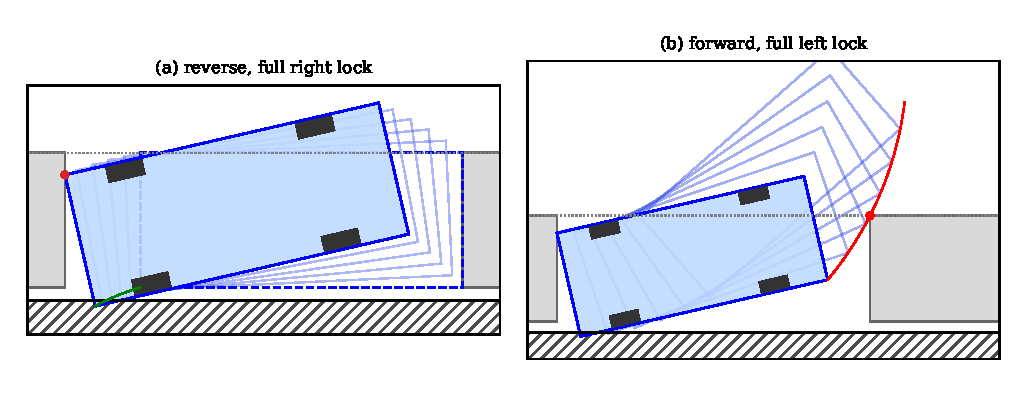
\includegraphics[width=\textwidth]{figures/fig_two_soft.pdf}
\caption{The two-manoeuvre exit of \cref{prop:two-soft} for the typical car ($L=\Lambda_2^{\rm s}=5.312$ m), with tyres drawn.
(a) Reverse with full right lock from the level position touching the car in front (dashed) until the rear bumper touches the car behind; the rear overhang passes over the curb.
(b) Forward exit with full left lock; the front curb-side corner (red trace) grazes $\Qf$.}
\label{fig:two-soft}
\end{figure}

\subsection{Three or more manoeuvres}
For more manoeuvres we repeated the zigzag searches of \cref{sec:zigzag,app:twenty} with the soft-curb collision test (\cref{app:numerics}).
For the typical car they give $\Lmins(3)\le5.088$, $\Lmins(4)\le4.978$, $\Lmins(5)\le4.906$ and $\Lmins(20)\le4.704$ m; \cref{tab:compare} lists all six cars.
The motions differ from the rigid ones.
The reverse manoeuvres are no longer stopped by the rear corner hitting the curb, but by the rear bumper meeting the car behind.
In the five- and twenty-manoeuvre motions of \cref{app:five-soft,app:twenty-soft}, for instance, the car is wedged between the two parked cars rather than between the curb and the car in front (compare \cref{app:five,app:twenty}).
In the twenty-manoeuvre motion the tyres never come closer than $16$ cm to the curb, and the body passes at most $5.2$ cm beyond the curb.

\subsection{Many manoeuvres}

\begin{proposition}\label{prop:asym-soft}
Assume the hypotheses of \cref{thm:asym}, $H<\min(b+\lambda,\,d_b+a)$, $m+\delta_s<w$ and
\begin{equation}\label{eq:mcond-soft}
  w-(m+\delta_s)\sec\psi>\ell\tan\frac\psi2\qquad\text{for }0<\psi\le\psi_{\max}.
\end{equation}
Then \cref{thm:mono,thm:asym} hold for the soft curb, with the same constant $K$.
That is, $\ell<\Lmins(n)\le\Lmins(1)$ for all $n$, and $\sqrt n\,(\Lmins(n)-\ell)\to K$.
\end{proposition}

\begin{proof}
The upper bound $\limsup_{g\to0}g^2N^{\rm s}(g)\le K^2$ follows from \cref{prop:asym-upper} and \eqref{eq:soft-le}.
For the lower bound we go through \cref{sec:asym}.
The curb is used only in \cref{lem:confine}, through lower bounds for the heights of the lowest corners.
In the soft-curb model, $\cTr_y\ge0$ and $\cTf_y\ge0$ give instead
\[
  \cFC_y\ge-\delta_s,\quad \cRL_y\ge(w-\delta_s)\cos\psi-(d_b-\lambda)\sin\psi\qquad(\psi\ge0),
\]
\[
  \cRC_y\ge-\delta_s,\quad \cFL_y\ge(w-\delta_s)\cos\psi-(d_f-\lambda)|\sin\psi|\qquad(\psi\le0).
\]
Hence, in the proof of \cref{lem:confine}(i), $\cRL$ (nose-up) and $\cFL$ (nose-down) still lie above the gap when $|\psi|\le\psi_1$ is small.
In case d and its nose-down analogue, the depth $m-\cFC_y$, respectively $m-\cRC_y$, is now at most $m+\delta_s$ instead of $m$.
The proof goes through with $m$ replaced by $m+\delta_s$ in the constants $c$ and $\psi_1$ and in the function $f$ of part (ii).
Part (ii) uses \cref{lem:soft-fit} instead of \cref{lem:fit}, and \eqref{eq:mcond-soft} instead of \eqref{eq:mcond}.
The rest of \cref{sec:asym} concerns configurations with $u\ge0$ and $|\psi|<cg$.
Their lowest points are at height at least $m-O(g)>0$, so the curb plays no role there in either model.
\end{proof}

Condition \eqref{eq:mcond-soft} holds by a wide margin for all six cars of \cref{tab:cars}.
The two models therefore have the same leading-order asymptotics.

\subsection{The flush problem}
In the soft-curb model the margin may be zero.
The flush problem is then not degenerate, unlike in the rigid model (\cref{prop:flush}).
For $m=0$ and the typical car, a parked car can tilt by at most $\psi_t=0.0073$ rad, which is less than $\beta_t$.
The binding constraint is therefore the swing of the rear tyre during the exit, as for the rear corner in \cref{thm:one}.
Numerically, the best one-manoeuvre exit then needs $5.856$ m.
This is the value $X(\psi)+\sqrt{\rho^2-(r_t-H)^2}$ at the heading $\psi$ with $Y(\psi)=r_t-H$, slightly below the classical $5.861$ m.
The two-manoeuvre exit of \cref{prop:two-soft} is not available for $m=0$, because \ref{T:tyre} fails.

\section{Rigid versus soft curb}\label{sec:compare}

\Cref{tab:compare} lists the slot lengths in both models for the six cars of \cref{tab:cars}, and \cref{fig:compare} plots them for the typical car.
By \eqref{eq:soft-le} no soft-curb value can exceed the corresponding rigid-curb value, and the computed values respect this.

\begin{table}[ht]
\centering\small
\begin{tabular}{@{}llccccc@{}}
\toprule
car & curb & $n=1$ & $n=2$ & $n=3$ & $n=4$ & $n=5$\\
\midrule
City car & rigid & 4.910 & 4.517 & 4.311 & 4.222 & 4.132\\
 & soft & 4.895 & 4.471 & 4.277 & 4.189 & 4.128\\
\addlinespace[2pt]
Compact & rigid & 5.686 & 5.271 & 5.126 & 5.024 & 4.911\\
 & soft & 5.664 & 5.186 & 4.971 & 4.872 & 4.815\\
\addlinespace[2pt]
Typical & rigid & 5.833 & 5.411 & 5.280 & 5.180 & 5.050\\
 & soft & 5.809 & 5.312 & 5.088 & 4.978 & 4.906\\
\addlinespace[2pt]
Mid-size sedan & rigid & 6.452 & 6.052 & 5.926 & 5.844 & 5.744\\
 & soft & 6.419 & 5.866 & 5.621 & 5.507 & 5.433\\
\addlinespace[2pt]
Large SUV & rigid & 6.877 & 6.393 & 6.288 & 6.187 & 6.069\\
 & soft & 6.840 & 6.231 & 5.959 & 5.831 & 5.758\\
\addlinespace[2pt]
Van & rigid & 7.543 & 6.969 & 6.850 & 6.734 & 6.597\\
 & soft & 7.503 & 6.794 & 6.480 & 6.330 & 6.253\\
\bottomrule
\end{tabular}
\caption{Slot lengths (in metres) with a rigid curb (\cref{tab:cars}) and with a soft curb, for margin $m=w/10$ and the tyre data of \cref{sec:model-soft}.
For $n=1$ the values are exact (\cref{thm:one,thm:one-soft}; for the city car the soft value is numerical).
For $n=2$ the soft values are $\Lambda_2^{\rm s}$ of \cref{prop:two-soft}; all entries with $n\ge2$ are upper bounds.}
\label{tab:compare}
\end{table}


\begin{figure}[ht]
\centering
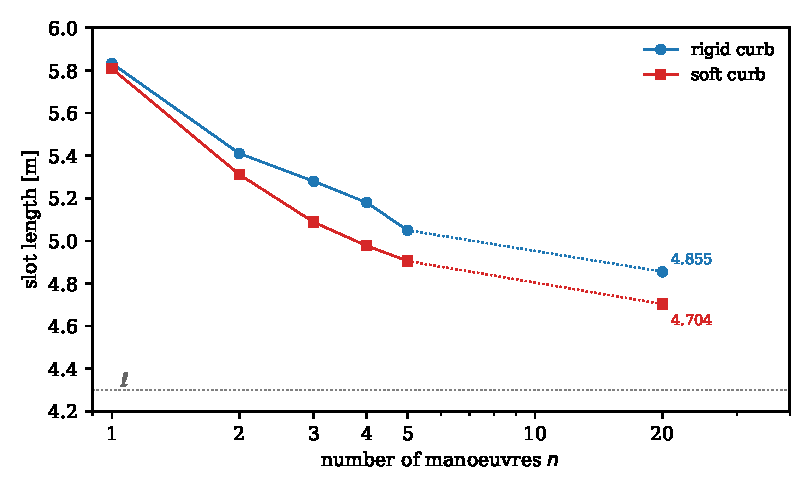
\includegraphics[width=0.8\textwidth]{figures/fig_compare.pdf}
\caption{Slot lengths with $n$ manoeuvres for the typical car, with a rigid curb (blue) and a soft curb (red).
The values for $n=1$ are exact; the others come from explicit strategies and are upper bounds.
The dotted segments only join $n=5$ to $n=20$.}
\label{fig:compare}
\end{figure}

\paragraph{One manoeuvre.}
The optimal single manoeuvres have the same shape in both models.
The car starts tilted nose-up, as far back and as high as possible, and drives out with full left lock while its front curb-side corner grazes $\Qf$.
Both slot lengths are values of the same function, $\Lmin(1)=\varphi_0(\psi_d)$ and $\Lmins(1)=\varphi_0(\psi_t)$; only the admissible tilt differs.
With a rigid curb the tilt is limited by the swing of the rear corner towards the curb during the turn.
With a soft curb the rear corner may pass over the curb, and the tilt is limited by the rear tyre touching the curb at rest.
The gain is small, $1.5$--$3.9$ cm for our six cars, because in both models the decisive constraint is the corner $\Qf$ of the car in front.
Both values are below the classical length $d_b+\sqrt{b^2+2Rw}$, by $2.8$ and $5.3$ cm for the typical car.

\paragraph{Two manoeuvres.}
Here the curb matters much more.
With a soft curb the textbook exit of \cref{prop:two-soft} is admissible: reverse with full right lock until the rear bumper touches the car behind, then leave with full left lock.
Its length $\Lambda_2^{\rm s}$ depends neither on the margin nor on the tyres.
With a rigid curb this exit would drive the rear corner into the curb.
The best rigid exit we know (\cref{prop:two-better}) therefore first turns the car slightly nose-down and needs three contacts.
The soft curb saves between $4.6$ and $18.6$ cm, and $9.9$ cm for the typical car.

\paragraph{Three to twenty manoeuvres.}
The rotation zigzags work in both models, but they are limited by different contacts.
With a rigid curb each reverse manoeuvre ends when the rear corner meets the curb.
With a soft curb it ends when the rear bumper meets the car behind.
For three to five manoeuvres the best soft-curb zigzags we found are $14$--$20$ cm shorter than the rigid-curb ones for the typical car, and up to about $40$ cm shorter for the van.
In \cref{tab:compare} the gain roughly grows with the rear overhang, the part of the car that swings towards the curb when it reverses: it is largest for the mid-size sedan, the large SUV and the van ($d_b\ge1$ m) and only a few centimetres for the city car ($d_b=0.55$ m).
With twenty manoeuvres the typical car needs $4.704$ m instead of $4.855$ m, and its motion is wedged between the two parked cars instead of between the curb and the car in front (\cref{app:twenty-soft,app:twenty}); the five-manoeuvre motions of \cref{app:five-soft,app:five} differ in the same way.

\paragraph{Many manoeuvres.}
By \cref{prop:asym-soft}, $\sqrt n\,(\Lmin(n)-\ell)$ and $\sqrt n\,(\Lmins(n)-\ell)$ have the same limit $K$.
Hence the ratio of the slacks $\Lmins(n)-\ell$ and $\Lmin(n)-\ell$ tends to $1$.
For large $n$ the car stays nearly level while it crawls out, its lowest point stays near the height $m$, and the curb plays no role.

\paragraph{The margin.}
With a rigid curb a positive margin is indispensable: for $m=0$ no slot length suffices (\cref{prop:flush}).
With a soft curb the flush problem is well posed, and for the typical car one manoeuvre then needs $5.856$ m.
A positive margin still helps: it allows a larger tilt of the starting position in \cref{thm:one-soft} ($\psi_t=0.0561$ instead of $0.0073$ rad for the typical car) and the two-manoeuvre exit of \cref{prop:two-soft}.

\paragraph{Which model applies?}
The soft-curb model describes a curb that the overhangs of the car can clear, with nothing behind it that they could hit.
In our motions the body passes at most $9$ cm beyond the curb for the typical car, and about $15$ cm for the largest cars.
The rigid-curb model describes a wall, or a curb too high for the overhangs.
For one manoeuvre the distinction is nearly irrelevant, since the two values differ by a few centimetres.
For two to five manoeuvres it is worth up to $40$ cm, depending on the car, and drivers who know that their overhangs clear the curb can use correspondingly shorter gaps.

\paragraph{Sensitivity to the tyre data.}
Our tyre data are typical values, not measurements of particular cars.
The two-manoeuvre value $\Lambda_2^{\rm s}$ does not depend on them, as long as \ref{T:tyre} and \ref{T:end} hold.
For the typical car the one-manoeuvre value changes by less than $1.6$ cm when $\delta_s$ ranges over $[0,5]$ cm and $\lambda$ over $[0.20,0.30]$ m: it stays between $5.802$ and $5.817$ m (\texttt{numerics/soft\_sens.py}).
For some of these tyres \cref{ass:soft} fails; there the numerical optimum exceeds $\varphi_0(\psi_t)$ by at most $0.2$ mm, as for the city car.
The multi-manoeuvre motions keep the tyres well away from the curb: for the six cars at least $6.7$ cm with two manoeuvres and at least $11$ cm with three to five.
They all remain free for the largest tyres of this range, $\delta_s=0$ and $\lambda=0.30$ m (\cref{app:numerics}).
Since the lowest tyre point moves down as $\lambda$ grows or $\delta_s$ shrinks, all our upper bounds with $n\ge2$ hold for every choice of tyre data in this range.

\section{Formal verification in Lean}\label{sec:lean}

The model and a large part of the results have been formalised in Lean~4 (version 4.35.0) with the Mathlib library (tag \texttt{v4.35.0}).
The development is in the directory \texttt{lean/} that accompanies this paper.
It has about 4400 lines in 19 files, builds with \texttt{lake build} (the separate file \texttt{AsymAxiom.lean} with \texttt{lake build Parking.AsymAxiom}), and contains no \texttt{sorry}.
This section explains what is verified, how the formal statements relate to the ones in the paper, and which parts are assumed.

\subsection{The formal model}
The file \texttt{Model.lean} transcribes \cref{sec:model}.
A \texttt{Car} carries $d_f,d_w,d_b,w,\theta$ with positivity and $\theta<\pi/2$.
A \texttt{Config} is a triple $(x,y,\psi)$, and the footprint is the image of $[-d_b,b]\times[-\frac w2,\frac w2]$ under the rigid motion.
The obstacles are the open sets of \cref{sec:model}: the curb half-plane $\{y<0\}$ and the two parked cars $\{x<0,\ m<y<H\}$ and $\{x>L,\ m<y<H\}$.
\texttt{Free}, \texttt{Parked} and \texttt{InLane} are the three classes of configurations, with \texttt{InLane} requiring the whole footprint in $\{y\ge H\}$ and $\psi\in\pi\mathbb Z$.

A \texttt{Manoeuvre} consists of a direction $d=\pm1$, a length $S\ge0$, an initial point, and a heading $\psi:\R\to\R$ with $|\psi(s)-\psi(t)|\le|s-t|/R$.
The position is defined by $P(s)=P(0)+d\int_0^s\e(\psi(\sigma))\dd\sigma$.
This is \cref{def:manoeuvre}: a heading is $1/R$-Lipschitz exactly when it is absolutely continuous with $|\psi'|\le1/R$ almost everywhere.
A parking motion is a list of at most $n$ manoeuvres with matching end points, all of whose configurations are free, starting in the lane and ending parked.
\texttt{Feasible c m n L} states that one exists, and $\Lmin(n)$ is defined as $\inf\{L>0:\ \texttt{Feasible c m n L}\}$.
Lean's real infimum of the empty set is $0$, not $+\infty$.
This is why the formal monotonicity statements below carry the hypothesis that some slot is feasible for the smaller number of manoeuvres.

\subsection{What is verified}
\Cref{tab:lean} lists the correspondence.
All theorems in its upper part depend only on the three standard axioms of Lean and Mathlib (\texttt{propext}, \texttt{Classical.choice}, \texttt{Quot.sound}), as reported by \texttt{\#print axioms}.

\begin{table}[ht]
\centering\small
\begin{tabular}{@{}>{\raggedright\arraybackslash}p{0.31\textwidth}>{\raggedright\arraybackslash}p{0.37\textwidth}>{\raggedright\arraybackslash}p{0.24\textwidth}@{}}
\toprule
Paper & Lean & Status\\
\midrule
\cref{lem:reversal} (time reversal) & \texttt{Manoeuvre.reverse}, \texttt{reverse\_config} & proved for single manoeuvres\\
\cref{lem:monoL} (monotonicity) & \texttt{Feasible.mono\_L}, \texttt{Feasible.mono\_n}, \texttt{Lmin\_antitone} & proved\\
\cref{lem:mirror,lem:fit} & \texttt{Manoeuvre.mirror}, \texttt{Manoeuvre.shift}, \texttt{OneAssumptions.heading\_near} & proved (\cref{lem:fit} under \cref{ass:one})\\
\cref{prop:flush} (zero margin) & \texttt{not\_feasible\_zero\_margin} & proved\\
\cref{lem:distance} (distance identity) & \texttt{Manoeuvre.distSq\_incr} & proved (increment form)\\
\cref{prop:one-upper} & \texttt{feasible\_one\_at\_}$\Lambda_1$ & proved\\
\cref{prop:one-forward} & \texttt{exit\_forward\_lower} & proved\\
\cref{prop:one-reverse} & \texttt{exit\_reverse\_lower} & proved, in the form $L\ge\Lambda_1$ under \cref{ass:one}\\
\cref{thm:one} & \texttt{feasible\_one\_iff}, \texttt{Lmin\_one} & proved, under slightly stronger hypotheses (see text)\\
$K^2=\int_0^w\dd u/r_*(u)$ & \texttt{K\_sq\_eq} & proved\\
pointwise calibration inequality; the integral and area identities behind \cref{lem:calib,lem:loop} & \texttt{calib\_pointwise}, \texttt{calib\_integral}, \texttt{loop\_area} & proved\\
\midrule
\cref{thm:asym} & \texttt{asym} & proved from \texttt{AsymLower}, \texttt{AsymUpper}\\
\cref{thm:mono} ($\Lmin(n)>\ell$ when some slot is feasible, $\Lmin(n)\to\ell$) & \texttt{len\_lt\_Lmin}, \texttt{Lmin\_tendsto} & proved from \texttt{AsymLower} (and \texttt{AsymUpper} for the limit)\\
\cref{prop:asym-lower,prop:asym-upper} & \texttt{AsymLower}, \texttt{AsymUpper} & stated, not proved\\
\cref{sec:several} (few manoeuvres) & --- & not formalised\\
\bottomrule
\end{tabular}
\caption{Results of the paper and their formal counterparts.}
\label{tab:lean}
\end{table}

\paragraph{The one-manoeuvre theorem.}
\Cref{ass:one} is the structure \texttt{OneAssumptions c m}.
It carries the auxiliary angles $\psi_{\rm fit},\psi_b,\psi_d,\gamma,\beta,\psi_n,\psi_u$ as data together with their defining equations, and the inequalities (A1)--(A7) as fields.
The structure is slightly stronger than \cref{ass:one}.
It also contains the standing assumptions $R>w/2$ and $m>0$, and the inequality $\psi_d\le\psi_{\rm fit}$, which the paper derives from \cref{prop:one-upper,lem:fit}.
In \ref{A:far} it uses $\log$ instead of $\log^+$ in \eqref{eq:Bback} and requires $Hb>\ell h_0$, so that the two agree.
These extra conditions hold for all cars considered in this paper.
The formal theorem is
\begin{align*}
  &\texttt{theorem feasible\_one\_iff (A : OneAssumptions c m) (L :}\ \R\texttt{) :}\\
  &\qquad\texttt{Feasible c m 1 L}\ \iff\ \texttt{A.}\Lambda_1\le\texttt{L},
\end{align*}
with $\texttt{A.}\Lambda_1=X(\psi_d)+\sqrt{\rho^2-(r-H)^2}$ as in \eqref{eq:Lambda1def}, and \texttt{Lmin\_one} gives $\Lmin(1)=\Lambda_1$.
The proof follows \cref{sec:one} step by step: the explicit exit, the normalisation by \cref{lem:mirror,lem:fit}, the forward bound with its nine steps, and the reverse bound.
Checking that a particular car satisfies \cref{ass:one} is a numerical computation (\cref{app:assumptions}) and is not part of the formal development.

Two technical choices differ from the written proofs, without changing the mathematics.
First, since the heading is only Lipschitz, derivative arguments along a manoeuvre are replaced by a Dini-type criterion.
A continuous function whose increments satisfy $f(z)-f(s)\le M_s(z-s)^2$ for $z>s$ is non-increasing.
For example, \cref{lem:distance} is used in the form
\[
  |C(z)-Q|^2-|C(s)-Q|^2\le 2\,(P(s)-Q)\cdot\e(\psi(s))\,\big(d(z-s)-R\sin(\psi(z)-\psi(s))\big)+M_s(z-s)^2 .
\]
Second, in \cref{prop:one-reverse} the Gronwall estimate together with the measure $S_-$ of the set of times with $\psi<0$ is replaced by a single monotone quantity.
For every $\varepsilon>0$ the function $P_x+c_\psi\frac{Rb}{\Rp}\log(h+\varepsilon)$ is non-increasing on $[0,\tau_r]$.
Letting $\varepsilon\to0$ gives the bound of the paper, with $\log$ in place of $\log^+$; this is where the condition $Hb>\ell h_0$ enters.

\paragraph{The asymptotic theorem.}
\Cref{prop:asym-lower,prop:asym-upper} are not formalised.
Their proofs rest on the confinement lemma, the exact description of the free windows, the calibration with all its error terms, and the construction of tilted S-curves with $O(g^2)$ tracking estimates.
These are long perturbation arguments, uniform in the slack $g$, with many constants, and formalising them would be a project of its own.
In Lean the two propositions are the predicates
\begin{align*}
  \texttt{AsymLower c m}&:\ \forall\varepsilon>0\ \exists g_0>0\ \forall g\in(0,g_0]\ \forall n,\ \texttt{Feasible c m n }(\ell+g)\Rightarrow K^2-\varepsilon\le g^2n,\\
  \texttt{AsymUpper c m}&:\ \forall\varepsilon>0\ \exists g_0>0\ \forall g\in(0,g_0]\ \exists n,\ g^2n\le K^2+\varepsilon\ \wedge\ \texttt{Feasible c m n }(\ell+g),
\end{align*}
i.e.\ $\liminf_{g\downarrow0}g^2N(g)\ge K^2$ and $\limsup_{g\downarrow0}g^2N(g)\le K^2$.
Theorem \texttt{asym} derives $\sqrt n\,(\Lmin(n)-\ell)\to K$ from these two hypotheses and the hypotheses of \cref{thm:asym}.
Theorem \texttt{len\_lt\_Lmin} derives $\ell<\Lmin(n)$ from \texttt{AsymLower} alone, for every $n$ for which some slot is feasible, and \texttt{Lmin\_tendsto} derives $\Lmin(n)\to\ell$ from both hypotheses.
The inequality $\Lmin(n)\le\Lmin(1)$ follows from \texttt{Lmin\_antitone} once some slot is feasible with one manoeuvre.
Parts of the analytic core of the two propositions are proved: the identity $K^2=\int_0^w\dd u/r_*(u)=4Rw-w^3/(6R)$, the pointwise calibration inequality, the integral identity $\int_0^1\big(s_+(\frac12-\zeta)^++s_-(\zeta-\frac12)^+\big)\dd\zeta=(s_++s_-)/8$ behind its integrated form, and the corresponding area identity for the ideal loop.

For readers who want the unconditional statements, the separate file \texttt{AsymAxiom.lean} declares a single, clearly labelled axiom \texttt{paper\_asym\_bounds}.
It asserts the two propositions under the hypotheses of \cref{thm:asym}.
From it the file derives \texttt{thm\_asym}, \texttt{thm\_mono\_limit} and \texttt{thm\_mono\_gt} (the last still with the feasibility hypothesis), and \texttt{\#print axioms} lists \texttt{paper\_asym\_bounds} for exactly these three theorems.
No other file imports it.

\paragraph{Not formalised.}
The two-manoeuvre constructions of \cref{sec:several} and all numerical values are not formalised.
Neither is the soft-curb variant of \cref{sec:soft,sec:compare}.

\section{Discussion}\label{sec:discussion}

\paragraph{Summary.}
For a slot bounded by a rigid curb and two parked cars standing at a margin $m$ from it, we have the following (for a soft curb see \cref{sec:compare}).
\begin{itemize}[nosep]
\item $\Lmin(1)$ is given exactly by \eqref{eq:Lam1}.
\item Two manoeuvres reduce the required length substantially.
\item The required slack decays like $K/\sqrt n$, with the universal constant $K=\sqrt{4Rw-w^3/(6R)}$.
\end{itemize}
In practical terms the asymptotics are discouraging: halving the slack quadruples the number of manoeuvres.
At $g=0.1$ m the leading-order count $K^2/g^2$ is about $2650$, and our simulated crawl uses $2507$ manoeuvres.
The regime of few manoeuvres is governed by a different mechanism (rotation zigzags) and is far more efficient per manoeuvre.

\paragraph{Rotation versus crawling.}
For moderate slack the car can turn nose-up a little at every manoeuvre.
Each reverse arc lowers the escape length $V$ of \cref{sec:several} until a final forward exit is possible.
For small slack the confinement lemma forbids turning, and the only way out is to crawl sideways by S-curves.
The crawl gains about $g^2/(4R)$ of lateral clearance per manoeuvre.
This lift does not depend on the overhangs, which is why $K$ involves only $R$ and $w$.
The correction $-w^3/(6R)$ comes from the tilted crawl once the car is more than halfway out.
Then the lane-side corners overhang the parked cars, and the effective window becomes a slanted parallelogram.

\paragraph{The role of the margin.}
With $m=0$ the problem as originally posed is degenerate (\cref{prop:flush}).
For $m\ge\varepsilon_b$ the one-manoeuvre answer depends on $m$ only through the tilt $\psi_d$.
The many-manoeuvre constant $K$ does not depend on $m$ at all.
If $0<m<\varepsilon_b$, a full-lock exit from any parked position would drive the rear corner into the curb.
We expect that the optimal single manoeuvre then contains a \emph{curb-sliding} arc of intermediate curvature and that $\Lmin(1)$ exceeds the classical value, but we have not proved this.

\paragraph{Variants.}
\begin{itemize}[nosep]
\item \emph{Parked cars of a different width.} The parked cars enter the analysis through the corners $\Qr,\Qf$ and the band $(m,H)$, and the proofs use $H-m=w$ throughout (for instance in the height variable $u\in[0,w]$ and in the windows of \cref{sec:asym}).
For parked cars of another width the windows change, and so does the constant $K$; we have not worked this out.
\item \emph{Soft curb.} This variant is treated in \cref{sec:soft,sec:compare}.
Its tyre model is deliberately simple: plan-view rectangles aligned with the car.
Our motions remain free when the front tyres are steered and when the tyres are enlarged within the range of \cref{sec:compare}.
The model ignores the height of the curb and of the overhangs, and anything behind the curb.
If the body may pass only a given distance beyond the curb, the problem lies between the two models; we have not treated it.
\end{itemize}

\paragraph{Open problems.}
\begin{enumerate}[nosep]
\item Determine $\Lmin(n)$ exactly for $n\ge2$.
Our numerical searches suggest that the optimal two-manoeuvre exit first reverses briefly with \emph{left} lock and then with right lock (\cref{conj:two}).
\item Find the second-order term of the asymptotics; simulations suggest $g^2N(g)=K^2-c_1g+o(g)$.
\item Characterise the crossover between rotation zigzags and crawling as a function of $n$.
\item Prove that $\Lambda_2^{\rm s}$ is optimal for two manoeuvres with a soft curb; our searches within the zigzag family did not find a shorter two-manoeuvre exit.
\end{enumerate}

\appendix
\section{Verification of \texorpdfstring{\cref{ass:one}}{Assumption}}\label{app:assumptions}

For the typical car ($d_f=0.9$, $d_w=2.6$, $d_b=0.8$, $w=1.8$, $\theta=35^\circ$, $m=0.18$, lengths in metres) the derived quantities are
\[
\begin{gathered}
  R=3.7132,\quad \Rm=2.8132,\quad \Rp=4.6132,\quad \rho=5.7906,\quad r=4.6820,\quad H=1.98,\\
  \varepsilon_b=0.0689,\quad \psi_{\rm fit}=0.04225,\quad \psi_d=0.03137,\quad \beta=0.17171,\quad \gamma=0.92175,\quad \psi_b=0.47852,
\end{gathered}
\]
and $\Lambda_1=5.83295$, $B_{\rm back}=8.200$.
Each inequality of \cref{ass:one} holds with a comfortable margin.
The tightest in relative terms is the first inequality of \ref{A:far}, $d_b\cos\psi_{\rm fit}-\Rp\sin\psi_{\rm fit}+\rho=6.395\ge\Lambda_1$ (a margin of $9.6\%$); next come the first inequality of \ref{A:min} ($5.059>3.588$), $B_{\rm back}\ge\Lambda_1$ and \ref{A:curbcase} ($3.947\ge2.702$).

We also checked \cref{ass:one} on the grid
\[
\begin{gathered}
  d_f\in\{0.6,0.8,1.0,1.2\},\quad d_w\in\{2.3,2.6,2.9,3.2\},\quad d_b\in\{0.5,0.7,0.9,1.1,1.3\},\\
  w\in\{1.6,1.75,1.9,2.05\},\quad \theta\in\{28^\circ,33^\circ,38^\circ,43^\circ\},
\end{gathered}
\]
always with $m=w/10$.
Of the $1280$ parameter sets, $1160$ satisfy $m\ge\varepsilon_b$, and $1129$ of those satisfy all of \ref{A:db}--\ref{A:far}.
The $31$ exceptions are short and very wide cars ($d_w=2.3$ together with $w\ge1.9$, mostly with $d_f=0.6$, or with $\theta=43^\circ$).
For these either $B_{\rm back}\ge\Lambda_1$ fails ($21$ sets) or the condition $H<\Rm+d_b$ of \ref{A:fit} fails ($12$ sets, two of them also in the first group); they are far from real passenger cars.
The check is a short script, \texttt{numerics/assumptions.py} in the accompanying repository.
It evaluates the inequalities as stated, except that it also requires $Hb>\ell h_0$, so that $\log^+=\log$ in \eqref{eq:Bback}; this conservative extra condition changes none of the counts.

\section{Other car configurations}\label{app:cars}

\Cref{tab:cars} lists slot lengths for six cars, from a small city car to a large van, always with margin $m=w/10$.
The third row is the typical car of \cref{tab:values}.
For every car we checked \cref{ass:one} with the script described in \cref{app:assumptions}, and all seven groups of inequalities hold, so the column $n=1$ is exact.

For the first three cars the hypotheses of \cref{prop:two-better} hold, and the two-manoeuvre exit was also confirmed by an exact simulation.
For the three larger cars the triple-contact equations \eqref{eq:tc1}--\eqref{eq:tc2} have their solution at $\alpha_1<\beta$, outside the range of the proposition.
Their two-manoeuvre entries come from the numerical search of \cref{app:numerics}, restricted to two manoeuvres.
The columns $n=3,4,5$ come from the same search, started from the optimal parameters of the typical car.
Every reported value was confirmed by simulating the complete exit (script \texttt{numerics/car\_table.py}).

\begin{table}[ht]
\centering\small
\setlength{\tabcolsep}{4pt}
\begin{tabular}{@{}l*{5}{c}cc*{5}{c}c@{}}
\toprule
& $d_f$ & $d_w$ & $d_b$ & $w$ & $\theta$ & $\ell$ & $R$ & $n=1$ & $n=2$ & $n=3$ & $n=4$ & $n=5$ & $K$\\
\midrule
City car & 0.65 & 2.35 & 0.55 & 1.65 & $37^\circ$ & 3.55 & 3.12 & 4.910 & 4.517 & 4.311 & 4.222 & 4.132 & 4.51\\
Compact & 0.85 & 2.60 & 0.75 & 1.78 & $36^\circ$ & 4.20 & 3.58 & 5.686 & 5.271 & 5.126 & 5.024 & 4.911 & 5.02\\
Typical & 0.90 & 2.60 & 0.80 & 1.80 & $35^\circ$ & 4.30 & 3.71 & 5.833 & 5.411 & 5.280 & 5.180 & 5.050 & 5.15\\
Mid-size sedan & 0.95 & 2.85 & 1.00 & 1.84 & $34^\circ$ & 4.80 & 4.23 & 6.452 & 6.052$^{*}$ & 5.926 & 5.844 & 5.744 & 5.55\\
Large SUV & 1.00 & 3.00 & 1.05 & 1.98 & $33^\circ$ & 5.05 & 4.62 & 6.877 & 6.393$^{*}$ & 6.288 & 6.187 & 6.069 & 6.03\\
Van & 1.00 & 3.40 & 1.10 & 2.00 & $31^\circ$ & 5.50 & 5.66 & 7.543 & 6.969$^{*}$ & 6.850 & 6.734 & 6.597 & 6.71\\
\bottomrule
\end{tabular}
\caption{Slot lengths (in metres) for parallel parking with $n$ manoeuvres, for six car configurations with margin $m=w/10$.
The column $n=1$ is the exact value $\Lmin(1)=\Lambda_1$ of \cref{thm:one}.
The column $n=2$ is $\Lambda_2^*$ from \cref{prop:two-better}; entries marked $^*$ are numerical, because there the double contact occurs before the rear corner passes the bottom of its circle ($\alpha_1<\beta$, cf.\ \cref{rem:two-other}).
The columns $n=3,4,5$ are the best rotation zigzags found.
All entries with $n\ge2$ are upper bounds for $\Lmin(n)$.
For large $n$, $\Lmin(n)=\ell+K/\sqrt n+o(n^{-1/2})$ by \cref{thm:asym}.}
\label{tab:cars}
\end{table}


Some trends are visible.
\begin{itemize}[nosep]
\item The extra length over the car, $\Lmin(1)-\ell$, grows from $1.36$ m for the city car to $2.04$ m for the van, mainly through the turning radius $R$, which enters $\Lambda_1$ through the term $\sqrt{\rho^2-(r-H)^2}$.
\item A second manoeuvre saves $0.39$--$0.57$ m, and five manoeuvres save $0.71$--$0.95$ m compared with one.
\item The classical formula $d_b+\sqrt{b^2+2Rw}$ overestimates $\Lmin(1)$ by $0.02$--$0.04$ m for all six cars.
\item The constant $K$ ranges from $4.5$ to $6.7$ m. For a small slack $g=L-\ell$ about $K^2/g^2\approx4Rw/g^2$ manoeuvres are needed, so this number is roughly proportional to the turning radius times the width.
\end{itemize}

\section{A five-manoeuvre parking motion}\label{app:five}

\Cref{fig:five} shows the best five-manoeuvre motion we found for the typical car, in the slot $L=5.050$~m of \cref{tab:zigzag} (more precisely $5.0497$~m).
This slot is only $0.75$ m longer than the car and $0.78$ m shorter than the one-manoeuvre slot $\Lmin(1)=5.833$ m.
For five manoeuvres the rotation zigzag of \cref{sec:zigzag} is far better than the crawl of \cref{sec:asym}, which in our simulations needs $28$ manoeuvres already for $L=5.3$ m (\cref{fig:values}).
The motion is drawn in forward (parking) time; it is the time reversal of the optimised exit (\cref{lem:reversal}).
In driving terms:
\begin{enumerate}[nosep]
\item reverse into the slot along an S-curve, first with full right lock and then with full left lock, until the rear curb-side corner touches the curb; the car now points $0.40$ rad ($23^\circ$) nose-up;
\item pull forward $0.16$ m with full right lock until the front curb-side corner touches the bumper of the car in front (tilt $0.36$ rad);
\item reverse $0.50$ m with full left lock until the rear corners touch the curb and the bumper of the car behind (tilt $0.22$ rad);
\item pull forward $0.47$ m, with full right lock and for the last $0.14$ m with full left lock, stopping $3$ mm short of the car in front (tilt $0.17$ rad);
\item reverse $0.65$ m with full left lock into the level parked position, against the car behind.
\end{enumerate}
Each manoeuvre turns the car further towards level.
There is no sideways slip: the rear wheels roll along their paths, which are tangent to them at every instant, while the overhangs behind the rear axle and in front of it swing sideways as the car turns.
The contacts show what limits each step: the curb and the car behind limit the reverse manoeuvres, and the car in front limits the forward ones.
The motion was checked with the exact collision test of \cref{app:numerics} (script \texttt{numerics/fig\_five.py}).

\begin{figure}[ht]
\centering
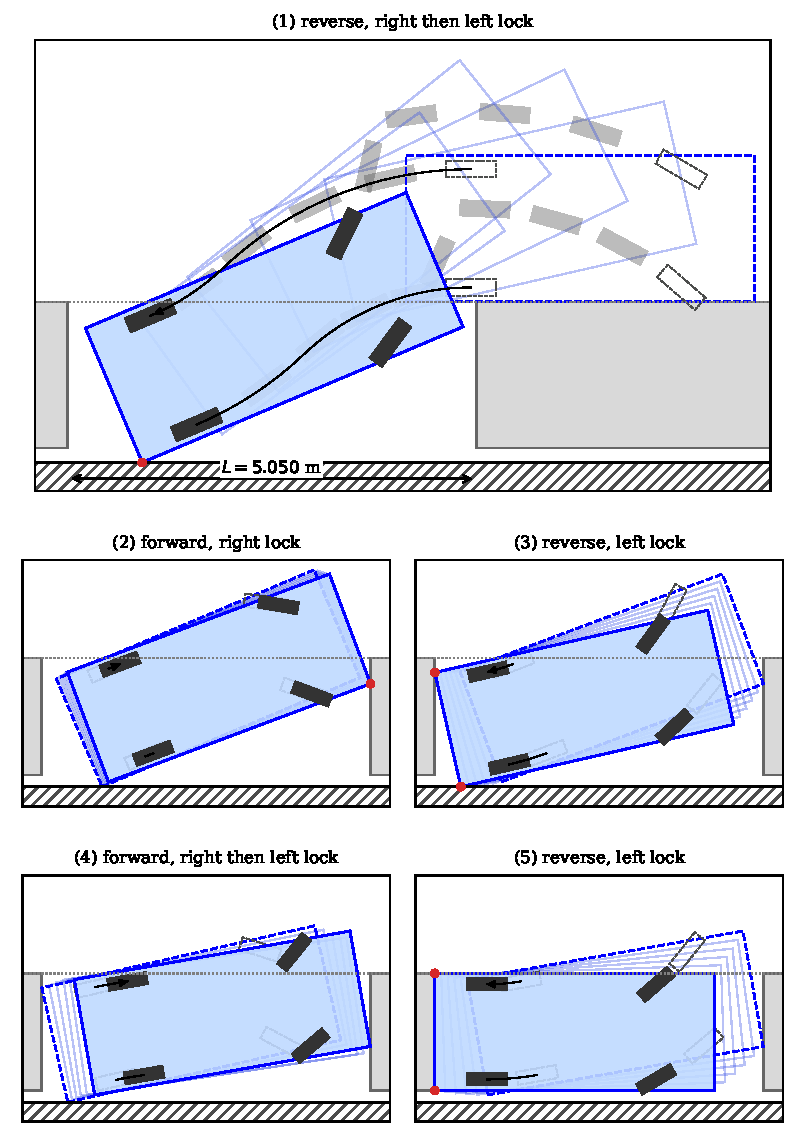
\includegraphics[width=\textwidth,height=0.8\textheight,keepaspectratio]{figures/fig_five.pdf}
\caption{The best five-manoeuvre parking motion found for the typical car, in a slot of length $L=5.050$ m.
Each panel shows one manoeuvre: start (dashed), intermediate positions (thin), end (filled), the paths of the two rear wheels with the direction of travel (black), and the contacts at the end of the manoeuvre (red dots).
The front wheels are drawn at the Ackermann angles of full lock.
Panel (1) is drawn at a smaller scale and also shows the wheels at the intermediate positions.}
\label{fig:five}
\end{figure}
\clearpage

\section{A twenty-manoeuvre parking motion}\label{app:twenty}

\Cref{fig:twenty} shows the same car parking with $20$ manoeuvres in a slot of length $L=4.855$ m.
This slot is $0.555$ m longer than the car, $0.195$ m shorter than the five-manoeuvre slot of \cref{fig:five}, and $0.98$ m shorter than $\Lmin(1)$.
We found it by searching \emph{contact zigzags}, which we describe as exits (the time reversals of parking motions).
Every full-lock arc is driven until the car touches the curb or a parked car, except for an optional left-lock arc of a fixed angle $a\in\{0,0.02,\dots,0.08\}$ rad before each reverse arc; the escape is tried before every manoeuvre.
The parked starting position, the direction of the first exit manoeuvre and $a$ were searched on a grid, which was then refined near the optimum, and bisection on $L$ located the shortest slot.
The best exit found has $a=0$.
Every manoeuvre was checked with the exact collision test (scripts \texttt{numerics/twenty\_search.py} and \texttt{numerics/fig\_twenty.py}).
The value is therefore an upper bound for $\Lmin(20)$.

The motion has three phases.
\begin{enumerate}[nosep]
\item The car reverses into the slot along an S-curve ($4.04$ m) and ends tilted by $26.7^\circ$, with its rear curb-side corner on the curb.
\item In manoeuvres 2--16 it is wedged between the curb and the car in front.
It alternately pulls forward with full right lock until its front curb-side corner touches the car in front, and reverses with full left lock until its rear curb-side corner touches the curb.
Each of these manoeuvres is only $2$--$10$ cm long and turns the car by $0.3^\circ$--$1.5^\circ$.
\item As the tilt decreases the wedge opens, and the steps grow: manoeuvres 17--20 are $19$--$41$ cm long and bring the car from $17.6^\circ$ to level. The reverse manoeuvres now end when the rear bumper touches the car behind, and the last forward manoeuvre ends in the level parked position.
\end{enumerate}
The number of manoeuvres needed grows very quickly as the slot shrinks.
In our searches $14$ manoeuvres suffice for $L=4.888$ m and $20$ for $L=4.855$ m, while for $L=4.80$ m the zigzag stalls: the rotation gained per manoeuvre tends to zero.
For comparison, the lateral crawl of \cref{sec:asym} needs $69$ manoeuvres for $L=4.9$ m and $97$ for $L=4.8$ m in our simulations (\cref{fig:values}); below about $4.85$ m it is the only strategy we know.
Accordingly, the asymptotic formula $\ell+K/\sqrt{n}$, which equals $5.45$ m for $n=20$, describes $\Lmin(n)$ only for much larger $n$.

\begin{figure}[p]
\centering
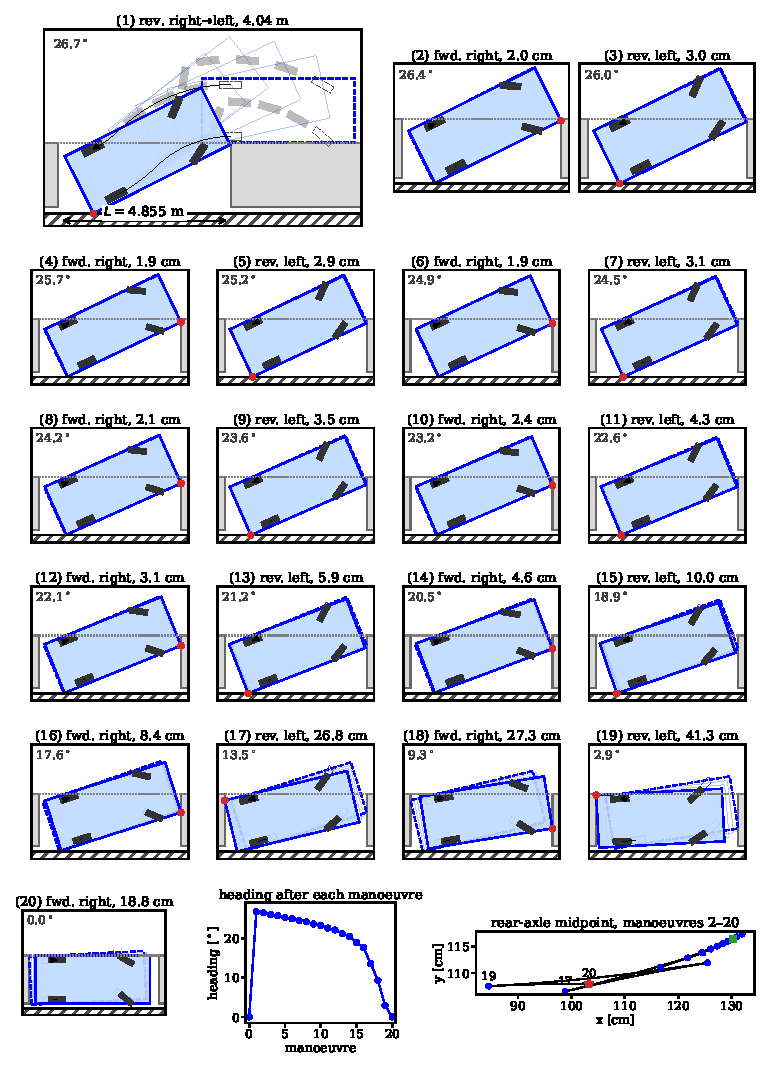
\includegraphics[width=\textwidth,height=0.84\textheight,keepaspectratio]{figures/fig_twenty.pdf}
\caption{The best twenty-manoeuvre parking motion found for the typical car, in a slot of length $L=4.855$ m.
Each panel shows one manoeuvre, drawn as in \cref{fig:five}: start (dashed), end (filled), wheels, rear-wheel paths, and contacts at the end (red dots).
The title gives the direction (fwd./rev.), the steering (full left or right lock) and the distance driven; the number in the corner is the heading at the end.
Panel (1) is drawn at a smaller scale.
Bottom: the heading after each manoeuvre, and the path of the rear-axle midpoint during manoeuvres 2--20 (green square: after manoeuvre 1; red star: parked).}
\label{fig:twenty}
\end{figure}
\clearpage

\section{A five-manoeuvre parking motion with a soft curb}\label{app:five-soft}

\Cref{fig:five-soft} shows the best five-manoeuvre motion we found for the typical car with a soft curb (\cref{sec:model-soft,sec:soft}), in a slot of length $L=4.906$~m (more precisely $4.9051$~m).
This is $0.14$ m less than the rigid-curb slot of \cref{fig:five}, only $0.61$ m longer than the car, and $0.90$ m shorter than the one-manoeuvre slot $\Lmins(1)=5.809$ m.
In driving terms:
\begin{enumerate}[nosep]
\item reverse into the slot along an S-curve, first with full right lock and then with full left lock, until the rear bumper touches the car behind; the car now points $0.38$ rad ($22^\circ$) nose-up, and its rear overhang passes up to $7.1$ cm beyond the curb;
\item pull forward $0.24$ m with full right lock until the front curb-side corner touches the car in front (tilt $0.32$ rad);
\item reverse $0.33$ m with full left lock until the rear bumper touches the car behind (tilt $0.23$ rad);
\item pull forward $0.34$ m with full right lock until the front curb-side corner touches the car in front (tilt $0.14$ rad);
\item reverse $0.52$ m with full left lock into the level parked position, against the car behind.
\end{enumerate}
The difference from \cref{fig:five} is that the curb no longer stops the reverse manoeuvres.
Each manoeuvre is a single full-lock arc driven until the car touches a parked car, so the car shuffles between the two parked cars; in the terminology of \cref{app:twenty} the motion is a contact zigzag with $a=0$.
The tyres stay at least $14.8$ cm from the curb.
We found the motion with the full search of \cref{app:numerics}.
All its parameters ended at their bounds, so the motion is determined by $L$, and we located the shortest slot by bisection on $L$.
The motion was checked with the exact collision test, also with the front tyres turned to the Ackermann angles and with the largest tyres of \cref{sec:compare} (scripts \texttt{numerics/fig\_five.py} with the argument \texttt{soft}, and \texttt{numerics/soft\_checks.py}).

\begin{figure}[ht]
\centering
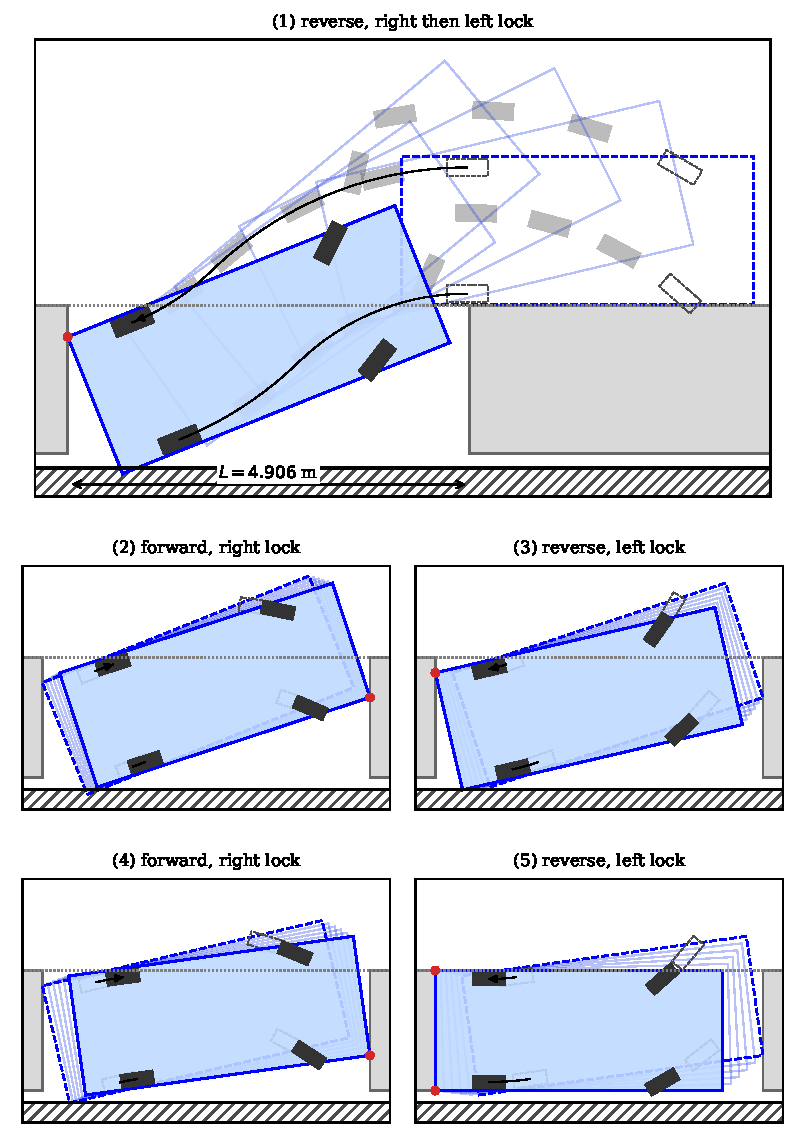
\includegraphics[width=\textwidth,height=0.8\textheight,keepaspectratio]{figures/fig_five_soft.pdf}
\caption{The best five-manoeuvre parking motion found for the typical car with a soft curb, in a slot of length $L=4.906$ m, drawn as in \cref{fig:five}.
The tyres are drawn with the data of \cref{sec:model-soft}, the front tyres at the Ackermann angles of full lock.
The bodywork may pass over the curb (hatched); the tyres may not.}
\label{fig:five-soft}
\end{figure}
\clearpage

\section{A twenty-manoeuvre parking motion with a soft curb}\label{app:twenty-soft}

\Cref{fig:twenty-soft} shows the typical car parking with $20$ manoeuvres and a soft curb, in a slot of length $L=4.704$ m (more precisely $4.7032$ m).
This is $0.15$ m less than with a rigid curb (\cref{fig:twenty}), $0.40$ m longer than the car, and $0.20$ m shorter than the soft-curb five-manoeuvre slot of \cref{fig:five-soft}.
We found it with the contact-zigzag search of \cref{app:twenty}, using the soft-curb collision test.
The best exit found starts from the parked position against the car in front, begins with a reverse manoeuvre and has $a=0$.
In parking time the car therefore ends with a forward manoeuvre against the car in front.
The motion has two phases.
\begin{enumerate}[nosep]
\item The car reverses into the slot along an S-curve ($4.10$ m) and ends tilted by $26.6^\circ$, with its rear bumper against the car behind; its rear overhang passes $5.2$ cm beyond the curb.
\item In manoeuvres 2--20 it is wedged between the two parked cars.
It alternately pulls forward with full right lock until its front curb-side corner touches the car in front, and reverses with full left lock until its rear bumper touches the car behind.
The steps grow as the tilt decreases.
Manoeuvres 2--12 are $4$--$6$ cm long and turn the car by $0.6^\circ$--$0.9^\circ$ each.
Manoeuvres 17--20 are $14$--$33$ cm long and bring the car from $13.1^\circ$ to level; the last one ends in the level parked position.
\end{enumerate}
Unlike the rigid-curb motion, this motion has no phase in which the car is wedged against the curb.
Its tyres stay at least $16$ cm from the curb, and from manoeuvre 15 on the whole body is above the curb line.
The motion was checked as in \cref{app:five-soft} (scripts \texttt{numerics/twenty\_search.py} and \texttt{numerics/fig\_twenty.py} with the argument \texttt{soft}).
The value is therefore an upper bound for $\Lmins(20)$.

\begin{figure}[p]
\centering
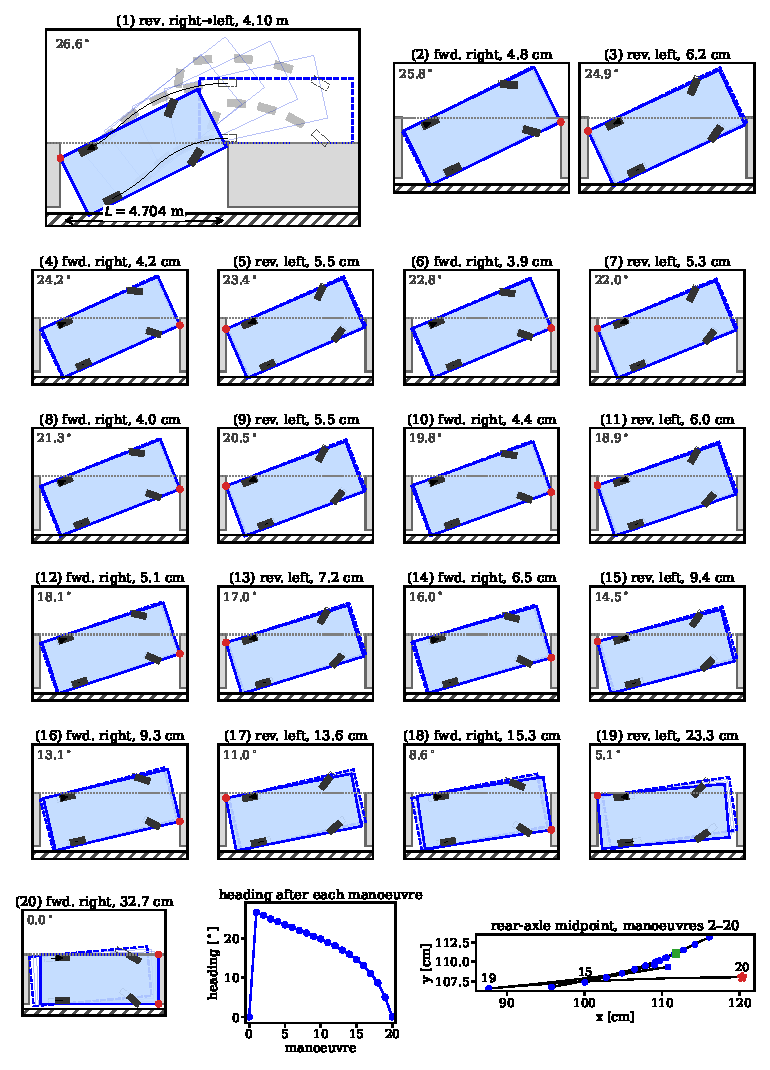
\includegraphics[width=\textwidth,height=0.84\textheight,keepaspectratio]{figures/fig_twenty_soft.pdf}
\caption{The best twenty-manoeuvre parking motion found for the typical car with a soft curb, in a slot of length $L=4.704$ m, drawn as in \cref{fig:twenty}, with the tyres of \cref{sec:model-soft}.
Panel (1) is drawn at a smaller scale.
Bottom: the heading after each manoeuvre, and the path of the rear-axle midpoint during manoeuvres 2--20 (green square: after manoeuvre 1; red star: parked).}
\label{fig:twenty-soft}
\end{figure}
\clearpage

\section{Numerical methods}\label{app:numerics}

\paragraph{Collision test.}
A configuration is tested exactly: each edge of the footprint is clipped against the open strips $\Or$, $\Of$, and the lowest corner is compared with the curb.
In the searches the configuration is sampled along each arc with step $2$--$3$ mm, and contact times are refined by bisection to $10^{-9}$ m; the figure scripts re-check each motion with $400$ samples per arc.
For the soft curb the lowest corner is replaced by the lowest corner of the tyre rectangles.

\paragraph{Strategy search.}
For $n\le6$ we parametrised exits by the starting position (level, at the top of the slot) and, for each manoeuvre, the fraction of the maximal collision-free length of its full-right-lock or forward full-left-lock arc, together with the angle (at most $0.1$ rad) of the optional left-lock arc of a reverse manoeuvre.
Forward manoeuvres were single full-left-lock arcs.
Reverse manoeuvres were either a single full-right-lock arc or a short full-left-lock arc followed by a full-right-lock arc.
For each trial length $L$ the parameters were optimised by differential evolution (with polishing) so as to maximise $L-V$ at the end; feasibility was then confirmed by simulating the final exit.
The minimal feasible $L$ was located by bisection.
The values are upper bounds for $\Lmin(n)$ and are rounded up to three decimals.
For \cref{tab:cars,tab:compare} a lighter version was used: $40$ generations without polishing, warm-started from the optimal parameters of the typical car, and stopped as soon as a verified exit was found.
For the typical car it reproduced the values for $n=3$ and $5$ and improved the value for $n=4$ from $5.184$ to $5.180$ m.
With a soft curb the light search gave $4.140$ m for the city car with five manoeuvres, more than the rigid-curb value $4.132$ m.
We therefore ran a second pass for this entry, warm-started from the car's own rigid-curb zigzag.
A rigid-curb motion is also free with a soft curb, so this pass can only improve a value; it gave $4.128$ m.
For the typical car the soft-curb values with $n=3,4,5$ come from the full search, as the rigid-curb values of \cref{tab:zigzag}.
It gave $5.088$, $4.978$ and $4.906$ m, against $5.089$, $4.988$ and $4.923$ m from the light search, which can therefore miss the best zigzag by up to $2$ cm.
In all three cases the optimal parameters lie at their bounds, so the motion is a contact zigzag in the sense of \cref{app:twenty}, determined by $L$; we then located the shortest slot by bisection on $L$.

\paragraph{Checks of the soft-curb motions.}
The script \texttt{numerics/soft\_checks.py} re-simulates the soft-curb motions behind \cref{tab:compare} and behind the soft-curb twenty-manoeuvre value with $400$ samples per arc, in three tyre models.
These are the model of \cref{sec:model-soft}, the same model with the front tyres turned to the Ackermann angles of the current full-lock arc, and, for $n\ge2$, the model with the largest tyres of \cref{sec:compare} ($\delta_s=0$, $\lambda=0.30$ m).
All motions are free in all three.
The script also reports the clearances quoted in \cref{sec:soft,sec:compare}.

\paragraph{Crawls.}
For \cref{tab:crawl} each manoeuvre is an S-curve of two full-lock arcs.
Its first angle is maximised by bisection under exact collision checks along the curve (40 samples per arc), with the end heading prescribed ($0$ for the plain crawl, $\mp\varpi(u)g/2$ for the tilted crawl).
The count stops when the car lies entirely in the lane.

% ---------------------------------------------------------------------------------------------
\section{Disclosure of irresponsible LLM use}\label{app:ai}

This work was carried out with substantial help from an LLM (Claude Opus~5.5, Anthropic), used as a coding and writing agent through Claude Code.
The author posed the problem, chose the margin model of \cref{sec:model} and directed the work.
Meanwhile a Discord server of the author, mathematicians, physicists and software engineers cheered the model on with pom-poms and encouraged it to continue.
Under this direction the model
\begin{itemize}[nosep]
\item derived the proofs and drafted the text and the figures;
\item wrote the numerical code in \texttt{numerics/} and ran the searches and simulations behind all tables and figures;
\item wrote the Lean~4 formalisation described in \cref{sec:lean};
\item reviewed the manuscript for errors in several rounds and revised it.
\end{itemize}
The author's further contributions were the requests for the tables, figures and variants, questions such as whether the rear tyres in \cref{fig:five} ought to be sliding (they are not), and a request to run the computations more gently, as they were slowing down the author's workstation.

The results differ in how they have been checked.
\begin{itemize}[nosep]
\item The statements formalised in Lean (\cref{sec:lean}) are machine-checked, up to the axioms and explicit hypotheses listed there.
That the Lean statements say what the theorems of the paper say was checked by the model that wrote both; where they differ, the differences are documented in \cref{sec:lean}.
\item All numerical values come from the scripts in \texttt{numerics/}, and every reported motion was re-simulated with the exact collision test of \cref{app:numerics}.
The values for $n\ge2$ are upper bounds obtained from explicit motions.
One value was found to be impossible, because it violated \eqref{eq:soft-le}, and was corrected (\cref{app:numerics}).
\item The remaining proofs, in particular those of \cref{sec:several,sec:asym,sec:soft}, have not been formally verified.
The model's own reviews found and repaired several gaps in them, among them one in the proof of \cref{prop:one-forward}; how many gaps they did not find is not known.
The proofs were eyeballed by the author and given a hopeful ``LGTM''.
\end{itemize}
The author does \emph{not} take full responsibility for the content of the paper.
Errors may be reported to the author, who will forward them to the model.

\begin{thebibliography}{9}
\bibitem{Blackburn}
S.~R. Blackburn, \emph{The geometry of perfect parking}, preprint, Royal Holloway, University of London, 2009.
\bibitem{Dubins}
L.~E. Dubins, On curves of minimal length with a constraint on average curvature, and with prescribed initial and terminal positions and tangents, \emph{Amer. J. Math.} \textbf{79} (1957), 497--516.
\bibitem{Laumond}
J.-P. Laumond, P.~E. Jacobs, M.~Ta\"ix and R.~M. Murray, A motion planner for nonholonomic mobile robots, \emph{IEEE Trans. Robotics and Automation} \textbf{10} (1994), 577--593.
\bibitem{ReedsShepp}
J.~A. Reeds and L.~A. Shepp, Optimal paths for a car that goes both forwards and backwards, \emph{Pacific J. Math.} \textbf{145} (1990), 367--393.
\bibitem{Vorobieva}
H.~Vorobieva, S.~Glaser, N.~Minoiu-Enache and S.~Mammar, Automatic parallel parking in tiny spots: path planning and control, \emph{IEEE Trans. Intelligent Transportation Systems} \textbf{16} (2015), 396--410.
\bibitem{WangEtAl}
X.~Wang, M.~Zhou, Z.~Liu and Z.~Ding, On minimum parking space required by automatic parallel parking, \emph{Sensors} \textbf{22} (2022), 795.
\end{thebibliography}

\end{document}
